% Version 0; preprint format; Outline of paper I by Song Huang
% 07/28 12839 words

\documentclass[fleqn,usenatbib,useAMS,english]{mnras}

% Packages
\usepackage{float}
\usepackage{natbib}
\usepackage{hhline}
\usepackage{multirow}
\usepackage{graphicx}
\usepackage{ae,aecompl}
\usepackage[T1]{fontenc}
\usepackage{deluxetable}
\usepackage{amssymb, amsmath}
\usepackage{newtxtext,newtxmath}
\usepackage[usenames, dvipsnames]{xcolor}
\usepackage{xcolor,colortbl}
\PassOptionsToPackage{hyphens}{url}
\usepackage{hyperref}
%\usepackage[nobiblatex]{xurl}
\usepackage{CJKutf8}

% Package Settings
\hypersetup{colorlinks=true,
            citecolor=MidnightBlue,
            linkcolor=MidnightBlue,
            filecolor=magenta,
            urlcolor=cyan}
\urlstyle{same}

% Figure extension
\DeclareGraphicsExtensions{.pdf,.png,.jpg}

% User definitions
%--------------- User Defined Commands ---------------------%
% Past papers
\defcitealias{Huang2018b}{Paper~I}	
\defcitealias{Huang2018c}{Paper~II}	


% Journals
\def\aa{{A\&A}}
\def\aas{{ A\&AS}}
\def\aj{{AJ}}
\def\annrev{{ARA\&A}}
\def\apj{{ApJ}}
\def\apjs{{ApJS}}
\def\mnras{{MNRAS}}
\def\nat{{Nature}}
\def\pasp{{PASP}}

% Song Huang's definition 
\def\arcsec{{\prime\prime}}
\def\arcmin{{\prime}}
\def\degree{{\circ}}
\def\h{\hskip -3 mm}
\def\amin{$^\prime$}
\def\asec{$^{\prime\prime}$}
\def\deg{$^{\circ}$}
\def\ddeg{{\rlap.}$^{\circ}$}
\def\dsec{{\rlap.}$^{\prime\prime}$}
\def\cc{cm$^{-3}$}
\def\flamb{erg s$^{-1}$ cm$^{-2}$ \AA$^{-1}$}
\def\flux{erg s$^{-1}$ cm$^{-2}$}
\def\fnu{erg s$^{-1}$ cm$^{-2}$ Hz$^{-1}$}
\def\hst{{\textit{HST}}}
\def\kms{km s$^{-1}$}
\def\lamb{$\lambda$}
\def\lax{{$\mathrel{\hbox{\rlap{\hbox{\lower4pt\hbox{${\sim}$}}}\hbox{$<$}}}$}}
\def\gax{{$\mathrel{\hbox{\rlap{\hbox{\lower4pt\hbox{${\sim}$}}}\hbox{$>$}}}$}}
\def\simlt{\lower.5ex\hbox{$\; \buildrel < \over {\sim} \;$}}
\def\simgt{\lower.5ex\hbox{$\; \buildrel > \over {\sim} \;$}}
\def\micron{{$\mu$m}}
\def\perang{\AA$^{-1}$}
\def\peryr{yr$^{-1}$}
\def\lsun{$L_\odot$} 
\def\sigs{$\sigma_*$}
\def\etal{{\ et al.}}
\newcommand{\lt}{<}
\newcommand{\gt}{>}

% ---- Commonly used notations ---- %
\def\mlratio{{$M_{\star}/L_{\star}$}}
\def\snratio{{$\mathrm{S}/\mathrm{N}$}}
\def\mden{{$\mu_{\star}$}}
\def\sb{mag~arcsec$^{-2}$}
\def\ser{{S\'{e}rsic}}
\def\cmodel{\texttt{CModel}}
\def\cmod{\texttt{CModel}}

% ----- COMMON NOTATIONS ABOUT MASS ----- %
\def\msun{$M_\odot$}
\def\mstar{{$M_{\star}$}}
\def\logms{{$\log_{10} (M_{\star}/M_{\odot})$}}
\def\logmh{{$\log_{10} (M_{\mathrm{Vir}}/M_{\odot})$}}
\def\logmvir{{$\log_{10} M_{\mathrm{vir}}$}}
\def\logmpeak{{$\log_{10} M_{\mathrm{peak}}$}}
\def\logminn{{$\log_{10} (M_{\star,10\mathrm{kpc}}/M_{\odot})$}}
\def\logmtot{{$\log_{10} (M_{\star,100\mathrm{kpc}}/M_{\odot})$}}
\def\logmout{{$\log_{10} (M_{\star,150\mathrm{kpc}}/M_{\odot})$}}
\def\logmmax{{$\log_{10} (M_{\star,\mathrm{max}}/M_{\odot})$}}
\def\logmcen{{$\log_{10} (M_{\star,\mathrm{cen}}/M_{\odot})$}}
\def\logmcmodel{{$\log_{10} (M_{\star,\mathrm{CMod}}/M_{\odot})$}}
\def\logm10{{$\log (M_{\star,10\ \mathrm{kpc}}/M_{\odot})$}}
\def\logm30{{$\log (M_{\star,30\ \mathrm{kpc}}/M_{\odot})$}}
\def\logm50{{$\log (M_{\star,50\ \mathrm{kpc}}/M_{\odot})$}}
\def\logm100{{$\log (M_{\star,100\ \mathrm{kpc}}/M_{\odot})$}}
\def\logmtot{{$\log (M_{\star,\mathrm{tot}}/M_{\odot})$}}
\def\logmsim{{$\log (M_{\star,\mathrm{3D}}/M_{\odot})$}}

% Stellar mass of all galaxies in the halo
\def\mall{{$M_{\star,\mathrm{all}}$}}
\def\mcen{{$M_{\star,\mathrm{cen}}$}}
\def\mgal{{$M_{\star,\mathrm{gal}}$}}
\def\mins{{$M_{\star,\mathrm{ins}}$}}
\def\mexs{{$M_{\star,\mathrm{exs}}$}}

% ---- Key definitions of halo mass ---- %
\def\mvir{{$M_{\mathrm{vir}}$}}
\def\mhalo{{$M_{\mathrm{vir}}$}}
\def\mpeak{{$M_{\mathrm{peak}}$}}
\def\mhost{{$M_{\mathrm{200b}}$}}
\def\mh200b{{$M_{\mathrm{200b}}$}}
\def\mh200c{{$M_{\mathrm{200c}}$}}

% ---- Aperture Stellar Mass ---- %
\newcommand{\maper}[1]{\ensuremath{M_{\star, {#1}\ \rm kpc}}}
\newcommand{\logmaper}[1]{{$\log (M_{\star, {#1}\ \rm kpc}/M_{\odot})$}}

\newcommand{\menve}[2]{{$M_{\star, [#1, #2]}$}}
\newcommand{\logmenve}[2]{{$\log (M_{\star, [#1, #2]}/M_{\odot})$}}

% Use italic font for in situ and ex situ
\def\insitu{{\textit{in situ}}}
\def\exsitu{{\textit{ex situ}}}
\def\ins{{\textit{in situ}}}
\def\exs{{\textit{ex situ}}}

% ---- Related to scatters of SHMR ---- %
% Scatter of log-M*_all at fixed halo mass (using stellar mass of all galaxies)
\def\sigms{{$\sigma_{M_{\star}}$}}
% Scatter of log-M*_cen at fixed halo mass (using stellar mass of central galaxies)
\def\sigmcen{{$\sigma_{\log M_{\star, {\rm cen}}}$}}
% Scatter of log-Mpeak at fixed stellar mass
\def\sigmpeak{{$\sigma_{\log M_{\mathrm{peak}}}$}}
% Scatter of log-M200b at fixed stellar mass
\def\sigmh{{$\sigma_{M_{\mathrm{vir}}}$}}
%\def\sigmh{{$\sigma_{\mathcal{M} | \mathcal{O}}$}}
% Scatter of log-Mvir at fixed stellar mass
\def\sigmvir{{$\sigma_{M_{\mathrm{vir}}}$}}
%\def\sigmvir{{$\sigma_{\mathcal{M} | \mathcal{O}}$}}


% ---- Fractions used in the model ---- %
% Ratio between the stellar mass of a galaxy and the stellar mass
% of all galaxies in the same halo
\def\fgal{{$\delta_{\rm gal}$}}
\def\fcen{{$\delta_{\rm cen}$}}
% Fraction of the in-situ component in stellar mass
\def\fins{{$\delta_{\rm ins}$}}
% Fraction of the ex-situ component in stellar mass 
\def\fexs{{$\delta_{\rm exs}$}}

% ---- Observed stellar mass from HSC images ---- %
% The 10 kpc aperture mass
\def\minn{{$M_{\star,10\ \mathrm{kpc}}$}}
% The 100 kpc aperture mass
\def\mtot{{$M_{\star,100\ \mathrm{kpc}}$}}
% The maximum 1-D profile mass
\def\mmax{{$M_{\star,\mathrm{max}}$}}
% Stellar mass measured by CModel
\def\mcmodel{\ensuremath{M_{\star,\mathrm{cmod}}}}
% \def\mcmodel{\ensuremath{M_{\star,\mathrm{cmod}}}}
% ASAP predicted halo mass
\def\masap{{$M_{\rm vir,\ ASAP}$}}

% Project related or softwares
\def\um{\texttt{UniverseMachine}}
\def\htools{\texttt{halotools}}
\def\smdpl{\texttt{SMDPL}}
\def\mdpl2{\texttt{MDPL2}}
\def\rockstar{\texttt{Rockstar}}
\def\emcee{\texttt{emcee}}
\def\asap{\texttt{ASAP}}
\def\redm{\texttt{redMaPPer}}
\def\camira{\texttt{CAMIRA}}
\def\galfit{{\tt GALFIT}}
\def\ised{{\tt iSEDfit}}
\def\mblack{{\tt MassiveBlackII}}
\def\illustris{{\tt Illustris}}
\def\tng{{\tt Illustris--TNG}}
\def\ellipse{\texttt{Ellipse}}
\def\iraf{\texttt{IRAF}}
\def\hscpipe{\texttt{hscPipe}}
\def\topn{{Top-$N$}}

% ---- Weak lensing related ---- %
\def\dsigma{{$\Delta\Sigma$}}
\def\rdsigma{{$R \times \Delta\Sigma$}}
\def\chisq{{$\chi^2$}}
\def\sqdeg{{deg$^2$}}

% ----- Editing and commenting ----- %
% Color
\definecolor{LightGray}{gray}{0.85}
\definecolor{Tab1}{RGB}{114, 158, 206}
\definecolor{Tab2}{RGB}{255, 158,  74}
\definecolor{Tab3}{RGB}{103, 191,  92}
\definecolor{Tab4}{RGB}{174, 199, 232}
\definecolor{Tab5}{RGB}{255, 187, 120}
\definecolor{Tab6}{RGB}{152, 223, 138}
\definecolor{Tab7}{RGB}{255, 152, 150}
\definecolor{Tab8}{RGB}{197, 176, 213}
\definecolor{hpurple}{HTML}{7E16DF}

% CB commands
%\newcommand{\M}[1]{\ensuremath{M_{\ast,\,\rm #1}}} % \, is a little space
\newcommand{\scatterMstarx}[1]{\ensuremath{\sigma_{\M{#1} | \Mhalo{}}}}
\newcommand{\Mhalo}{\ensuremath{M_{\rm vir}}} 
\newcommand{\obsSym}{\ensuremath{{\mathcal{O}}}}
\newcommand{\haloSym}{\ensuremath{{\mathcal{M}}}}
\newcommand{\slope}{\ensuremath{\alpha}}
\newcommand{\intercept}{\ensuremath{\pi}}
\newcommand{\hmf}{\Phi(\mu)}
\newcommand{\scatterObsSymMhalo}{\ensuremath{\sigma_{\mathcal{O} | \mathcal{M}}}}
\newcommand{\scatterMhaloObsSym}{\ensuremath{\sigma_{\mathcal{M} | \mathcal{O}}}}
\newcommand{\eg}{{\it e.g.,\/}}
\def\sighalo{{$\sigma_{M_{\rm vir}}$}}

% Commenting:
\newcommand{\xxx}[1]{\textcolor{red}{\textbf{XXX}}}
\newcommand{\todo}[1]{\textcolor{BrickRed}{\textbf{~#1}}}
\newcommand{\plan}[1]{\textcolor{Sepia}{#1}}
\newcommand{\addref}{{\textcolor{red}{REF}}}
\newcommand{\note}[2]{\textcolor{blue}{\textbf{[Comment (#1): #2]}}}
\newcommand{\alexie}[1]{\textcolor{blue}{\textbf{[Alexie: #1]}}}
\newcommand{\chris}[1]{\textcolor{PineGreen}{\textbf{[Chris: #1]}}}
\newcommand{\song}[1]{\textcolor{Cyan}{\textbf{[Song: #1]}}}
\newcommand{\susan}[1]{\textcolor{Bittersweet}{\textbf{[Susan: #1]}}}
\newcommand{\update}[1]{\textcolor{PineGreen}{#1}}
\newcommand{\aph}[1]{\textcolor{hpurple}{[APH: #1]}}
\newcommand{\jul}[1]{\textcolor{teal}{[JUL: #1]}}


%% ---------------------------------------------------------------------------------------------- %%
%% Title and Affiliations
%% ---------------------------------------------------------------------------------------------- %%
\title[Outer Galaxy Mass as a Halo Mass Proxy]{
    The Outer Stellar Mass of Massive Galaxies: A Simple Tracer of Halo Mass with Scatter 
    Comparable to Richness and Reduced Projection Effects}

\author[S. Huang et al.]{
        Song Huang$^{1,2}$\thanks{E-mail: sh19@princeton.edu (SH)},
        Christopher Bradshaw$^{2}$,
        Alexie Leauthaud$^{2}$,
        Andrew Hearin$^{3}$,
        \newauthor
        Peter Behroozi$^{4}$,
        Joseph DeRose$^{2}$,
        Johannes Lange$^{2}$,
        Jenny Greene$^{1}$,
        Joshua S. Speagle (\begin{CJK*}{UTF8}{bsmi}沈佳士\ignorespacesafterend\end{CJK*})$^{5,6,7}$\\
        $^{1}$Department of Astrophysical Sciences, Peyton Hall,
              Princeton University, Princeton, NJ 08540, USA \\
        $^{2}$Department of Astronomy and Astrophysics, University of California
              Santa Cruz, 1156 High St., Santa Cruz, CA 95064, USA\\
        $^{3}$Argonne National Laboratory, Argonne, IL 60439, USA\\
        $^{4}$Department of Astronomy and Steward Observatory, University of Arizona,
              Tucson, AZ 85721, USA\\
        $^{5}$Department of Statistical Sciences, University of Toronto, Toronto, M5S 3G3, Canada\\
        $^{6}$David A. Dunlap Department of Astronomy \& Astrophysics, University of Toronto, Toronto, M5S 3H4, Canada\\
        $^{7}$Dunlap Institute for Astronomy \& Astrophysics, University of Toronto, Toronto, M5S 3H4, Canada
        }

%% ---------------------------------------------------------------------------------------------- %%
\date{Accepted XXX. Received YYY; in original form ZZZ}
\pubyear{2020}


%% ---------------------------------------------------------------------------------------------- %%
%% Header and Version
%% ---------------------------------------------------------------------------------------------- %%

\begin{document}

\label{firstpage}
\pagerange{\pageref{firstpage}--\pageref{lastpage}}

\maketitle

%% ---------------------------------------------------------------------------------------------- %%
%% Abstract and Keywords
%% ---------------------------------------------------------------------------------------------- %%

\begin{abstract}
    
    Using weak gravitational lensing data from the Hyper Suprime-Cam Subaru Strategic Program
    (HSC survey), we study the potential of different stellar mass measurements in tracing halo
    mass.
    We consider galaxies with \logms{}$>11.5$ at $0.2 < z < 0.5$ with carefully measured light profiles,
    and clusters from the \redm{} and \camira{} richness-based algorithms.
    We devise a method (the ``\topn{} test'') to evaluate the scatter in the halo mass-observable
    relation for different tracers, and to inter-compare halo mass proxies in four number density bins using stacked
    galaxy-galaxy lensing profiles.
    This test reveals three key findings. Stellar masses based on \cmodel{} magnitudes and luminosity within
    $R<$30 kpc are poor tracers of halo mass. In contrast, the stellar mass of the outer envelope is an excellent halo
    mass proxy. The stellar mass within $R=[50,150]$ kpc,  \menve{50}{150}, has performance comparable to the
    state-of-the-art richness-based cluster finders at \logmvir{}$\gtrsim 14.0$ and could be 
    a better halo mass tracer at lower halo masses. Finally, using N-body simulations, we find that the lensing profiles of massive halos selected
    by \menve{50}{150} are consistent with the
    expectation for a sample without noticeable projection or mis-centering effects. Richness-selected clusters, on the other hand, display an excess at $R\sim 1$ Mpc in their 
    lensing profiles, which may suggest a more significant impact from selection biases.
    These results suggest that \mstar{}-based tracers have distinct advantages in
    identifying massive halos, which could open up new avenues 
    for cluster cosmology.

\end{abstract}

% TODO: Need updates!
\begin{keywords}
    cosmology: observations --
    gravitational lensing: weak --
    galaxies: structure --
    galaxies: cluster: general --
    galaxies: haloes
\end{keywords}


%% ---------------------------------------------------------------------------------------------- %%
%% Main Text
%% ---------------------------------------------------------------------------------------------- %%

%% ---------------------------------------------------------------------------------------------- %%
%% Introduction
%% ---------------------------------------------------------------------------------------------- %%

\section{Introduction}
    \label{sec:intro}
    
    With the rapid developments of multi-wavelength sky surveys, galaxy clusters
    have become increasingly important for cosmology and galaxy-halo connection studies.
    As the rare highest density peaks of the matter density distribution, galaxy clusters 
    have long been recognized as powerful probes of the mean cosmic matter density 
    ($\Omega_{\rm m}$), the amplitude of power spectrum ($\sigma_{8}$), and the cosmic expansion
    history (e.g.,
    \citealt{Evrard1989, Peebles1989, White1993, Viana1996, Wang1998}; 
    see \citealt{Allen2011, Kravtsov2012, Weinberg2013} for recent reviews).
    The abundance of galaxy clusters and their redshift evolution, the spatial distribution of 
    clusters, and the total mass distributions around the clusters all encode valuable 
    cosmological information (e.g., \citealt{Haiman2001, Holder2001, Vikhlinin2009b, Rozo2010, 
    Benson2013, Mantz2014, Bocquet2019, Abbott2020, To2021a, To2021b, Wu2021}).
    Meanwhile, massive galaxy clusters are also promising laboratories to study the boundary of
    dark matter halos (e.g., \citealt{Diemer2014, More2015b,
    More2016, Chang2018, Shin2019, Zurcher2019, Tomooka2020})\footnote{Please see
    \url{http://www.benediktdiemer.com/research/splashback/} for a more complete list of
    reference on this topic.} and investigate halo assembly bias (e.g., \citealt{Miyatake2016,
    Zu2017}).
    To achieve these goals, a reliable ``cluster finder'' that can identify galaxy clusters 
    is fundamental.
    Meanwhile, the ability of correctly ``weighing'' the clusters through 
    carefully calibrated halo mass--observable relations is also critical.
    
    Thanks to the advent of large optical surveys such as the Sloan Digital Sky Survey (SDSS,
    \citealt{York2000, SDSSDR7, SDSSDR16})\footnote{\url{https://www.sdss.org/}}, 
    the Dark Energy Survey (DES, \citealt{DES2016, Abbott2018,
    DES2021})\footnote{\url{https://www.darkenergysurvey.org/}}, and the Hyper Suprime-Cam Subaru
    Strategic Program (HSC-SSP,
    \citealt{Miyazaki2012, HSC-SSP, HSC-DR1,
    HSC-DR2})\footnote{\url{https://hsc.mtk.nao.ac.jp/ssp/}}, not only optical cluster finders
    are now wildly used to provide large samples of galaxy
    clusters across a wild range of redshift and halo mass (e.g., \citealt{Kepner1999,
    GladdersYee2000, Koester2007, Hao2010, Wen2012, Rykoff2014, Oguri2018, Aguena2021, Wen2021,
    Zou2021}),
    weak gravitational lensing is also regarded
    as the most promising approach to directly calibrate the mass-observable relations 
    (e.g., \citealt{Becker2011, vonderLinden2014, Applegate2014, Applegate2016, Okabe2016,
    Grandis2019}; also see \citealt{Umetsu2020b} for a recent review).
    Among the optical cluster finders, red--sequence based methods such as the 
    \redm{} (e.g., \citealt{Rykoff2014, Rozo2014, Rozo2015a, Rozo2015b, Rykoff2016}) and 
    \camira{} (e.g., \citealt{Oguri2014, Oguri2018}) have enjoyed the most success.
    These algorithms rely on the richness of the quiescent cluster members that form a 
    tight luminosity--colour sequence (e.g., \citealt{Bower1992, Kodama1997, Bell2004}) to
    identify galaxy clusters over a wide redshift and halo mass range.
    The richness estimates are then used to calibrate the mass--observable relation for 
    cosmological analysis, often with the help of gravitational lensing data (e.g.,
    \citealt{Baxter2016, Farahi2016, Simet2017, Melchior2017, Murata2018, McClintock2019}).
    
    However, red-sequence cluster finders (or any richness-based optical cluster finder) and
    the weak lensing calibrations of \mvir{}--richness relations suffer from systematics 
    such as the anisotropic selection bias (including both projection bias and orientation
    bias; e.g., \citealt{NohCohn2012, Dietrich2014, Osato2018, Herbonnet2019}) and 
    mis-centering effect (e.g., \citealt{Saro2015, Zhang2019b}).
    Among these systematic biases, the projection effect arising from structures surrounding the
    clusters in the line-of-sight direction is the most prominent and annoying one (e.g.,
    \citealt{Cohn2007, Erickson2011, Farahi2016, Zu2017, Busch2017, Costanzi2019, 
    Sunayama2019, Sunayama2020}).
    In richness-based cluster catalog, projection effect often manifests as the contamination of
    lower mass clusters at a given richness value (e.g., \citealt{Ge2019, Grandis2021, Myles2021}).
    It plagues the search for evidence of assembly bias in clusters (e.g., \citealt{Zu2017,
    Sunayama2019}) and can bias the estimate of splashback radius (e.g., \citealt{Busch2017,
    Sunayama2019}).
    More importantly, projection effect can significantly complicates the calibration of 
    mass-richness relation, hence impacts the cosmological inference (
    e.g., \citealt{Erickson2011, Costanzi2019, Sunayama2020, Wu2021}).
    In \citet{DES2020}, the authors conclude that the projection effect alone can lead to 
    a $\sim 20$\% over-estimate of halo mass in a given richness bin, and bias
    the cosmological parameters to an extent that it creates an apparent ``tension'' with
    the Planck 2018 results (e.g., \citealt{PLANCK2020})..
    Currently, it is still difficult to evaluate the impact of projection effect and
    calibrate its mitigation for richness-based cluster finders as it requires realistic mock
    catalogs of cluster galaxies with red-sequences consistent with observations, which 
    is not an easy task (e.g., \citealt{DeRose2019})


    While sophisticated methods that can marginalize over projection effect are being developed
    (e.g., \citealt{To2021a}) for cosmological inference, it is also tempting to search for
    complimentary optical cluster finders that suffer less from the projection effect.
    Halo mass proxies that uses the stellar mass of member galaxies are also affected
    by projection effect (e.g., \citealt{Palmese2020, Bradshaw2020}), but the massive central
    galaxy (or the brightest cluster galaxy, BCG) could provide an promising alternative.
    Firstly, the stellar mass of the massive central galaxies follow a 
    well-established stellar-halo 
    mass relation (SHMR, e.g., \citealt{Leauthaud2012, Tinker2017, Kravtsov2018}; also see
    \citealt{Wechsler2018} for a recent review) with moderate scatter at the high-mass end (e.g.,
    \citealt{More2009, Leauthaud2012, Reddick2013, Zu2015, Lehmann2017, Kravtsov2018}).
    Traditionally, the shallow slope of the halo mass-stellar mass relation stops 
    it from being considered as a competitive halo mass proxy.
    However, this impression could be partially caused by poorly measured luminosity of massive 
    galaxies in large surveys (e.g., \citealt{Bernardi2013, Huang2018b}.
    Recently, deep imaging surveys reveal the potential of using stellar mass measured to very
    large radius as an improved halo mass proxy (e.g., \citealt{Huang2018c, SampaioSantos2021}).
    In \citet{Huang2020}, we also demonstrate that a simple phenomenological model based on
    stellar masses measured within two apertures can further improve of this halo proxy.
    Additionally, the diffuse envelope around a BCG (often referred to as the intra-cluster
    light, or ICL) also show interesting connection to the dark matter halo of the cluster
    (e.g., \citealt{Montes2018, Montes2019, Zhang2019b, Furnell2021}).
    
    For these reasons, we want to revisit the possibility of using massive central galaxies 
    as ``cluster finders'' with the help from deep imaging data and high-quality galaxy-galaxy 
    lensing measurements from HSC.
    We design a so-called \topn{} test to evaluate their relative performance as halo mass proxies.
    In the \topn{} test, we compare the stacked galaxy--galaxy lensing profiles
    of ``clusters'' selected by different halo mass proxies within the number density bin
    (e.g., \citealt{Reyes2008}).
    With the help of cosmological simulation, we also infer the scatter of halo mass in each density
    bin by assuming a $\log$--linear halo mass-observable relation with constant Gaussian 
    scatter.
    The comparison of the lensing profiles from simulation and the ones in observation also help
    inform us whether the underlying cluster sample satisfies this simple assumption.
    
%% ---------------------------------------------------------------------------------------------- %%
%% Brief mention of key results
%% ---------------------------------------------------------------------------------------------- %%

%    In this work, we use deep imaging data and high-quality galaxy-galaxy lensing measurements
%    galaxy-halo connection of massive galaxies.
%    While \mstar{} based on default photometry from imaging survey pipeline such as the
%    well-known \cmodel{} photometry often fail to serve as useful \mvir{} proxy, \mstar{}
%    within very large aperture (e.g., within 100 kpc) is a much better choice.
%    Moreover, \mstar{} within the outskirt of a massive galaxy (e.g., \mstar{} within 50 to 100 kpc)
%    is a potentially competitive \mvir{} tracer when compared to the well-adopted richness of
%    red-sequence galaxies cluster finders.
%    We also find that the galaxy-galaxy lensing \dsigma{} profiles of massive halos selected
%    using \mstar{}-based proxies can be well-described using a simple model based on $\log$-linear
%    \mvir{}-observable relation with Gaussian scatter.
%    Meanwhile, with the same number density threshold, the \dsigma{} profiles of richness-selected
%    clusters show systematic deviations from such model predictions and the \mstar{}-based profiles
%    that could be caused by additional systematic issues such as the projection effect or
%    halo assembly bias.

%% ---------------------------------------------------------------------------------------------- %%
%% Structure of the paper
%% ---------------------------------------------------------------------------------------------- %%

    Here is the structure of this work:
    In the method section \S \ref{sec:method}, we will first explain the
    philosophy behind the \topn{} test (\S \ref{sec:topn_intro}) and the methodology for
    comparing different \mhalo{} proxies using the scatter of \mhalo{} estimated from the
    stacked \dsigma{} profiles (\S \ref{sec:model}).
    Then we introduce the data (\S \ref{sec:data}) used in this work along with the key
    measurements (\S \ref{sec:measure}), including different \mstar{} measurements based on
    1-D profiles (\S \ref{sec:1d_prof}) and the \dsigma{} lensing profiles (\S \ref{sec:dsigma}).
    We also briefly summarize the different \mhalo{} proxies used in the \topn{} tests
    (\S \ref{sec:proxies}).
    We summarize the key results in \S \ref{sec:result}, including a
    brief demonstration of impact from satellite galaxies (\S \ref{sec:satellite}), a concise
    review of the performance of different \mhalo{} proxies, and the general trend of
    \sigmh{} with number density (\S \ref{sec:topn_results}).
    We then pay special attention to the comparison between \mstar{}- and richness-based
    \mhalo{} proxies (\S \ref{sec:mstar_vs_richness}).
    We discuss the physical implications of these results along with their limitations and
    caveats in \S \ref{sec:discussion}.
    Finally, in \S \ref{sec:summary}, we summarize the lessons learned here and point out a few
    future directions to explore.

%% ---------------------------------------------------------------------------------------------- %%
%% Important assumptions and definitions
%% ---------------------------------------------------------------------------------------------- %%

    For cosmology, we assume $H_0$ = 70~km~s$^{-1}$ Mpc$^{-1}$,
    ${\Omega}_{\rm m}=0.3$, and ${\Omega}_{\rm \Lambda}=0.7$.
    Stellar mass (\mstar{}) is derived using a Chabrier initial mass function
    (IMF; \citealt{Chabrier2003}).
    And we use $M_{\rm vir}$ for dark matter halo mass (\mhalo{}) as
    defined in \citealt{BryanNorman1998}.

%% ---------------------------------------------------------------------------------------------- %%
%% Figure: the philosophy of Top N tests
%% ---------------------------------------------------------------------------------------------- %%
    \begin{figure*}
    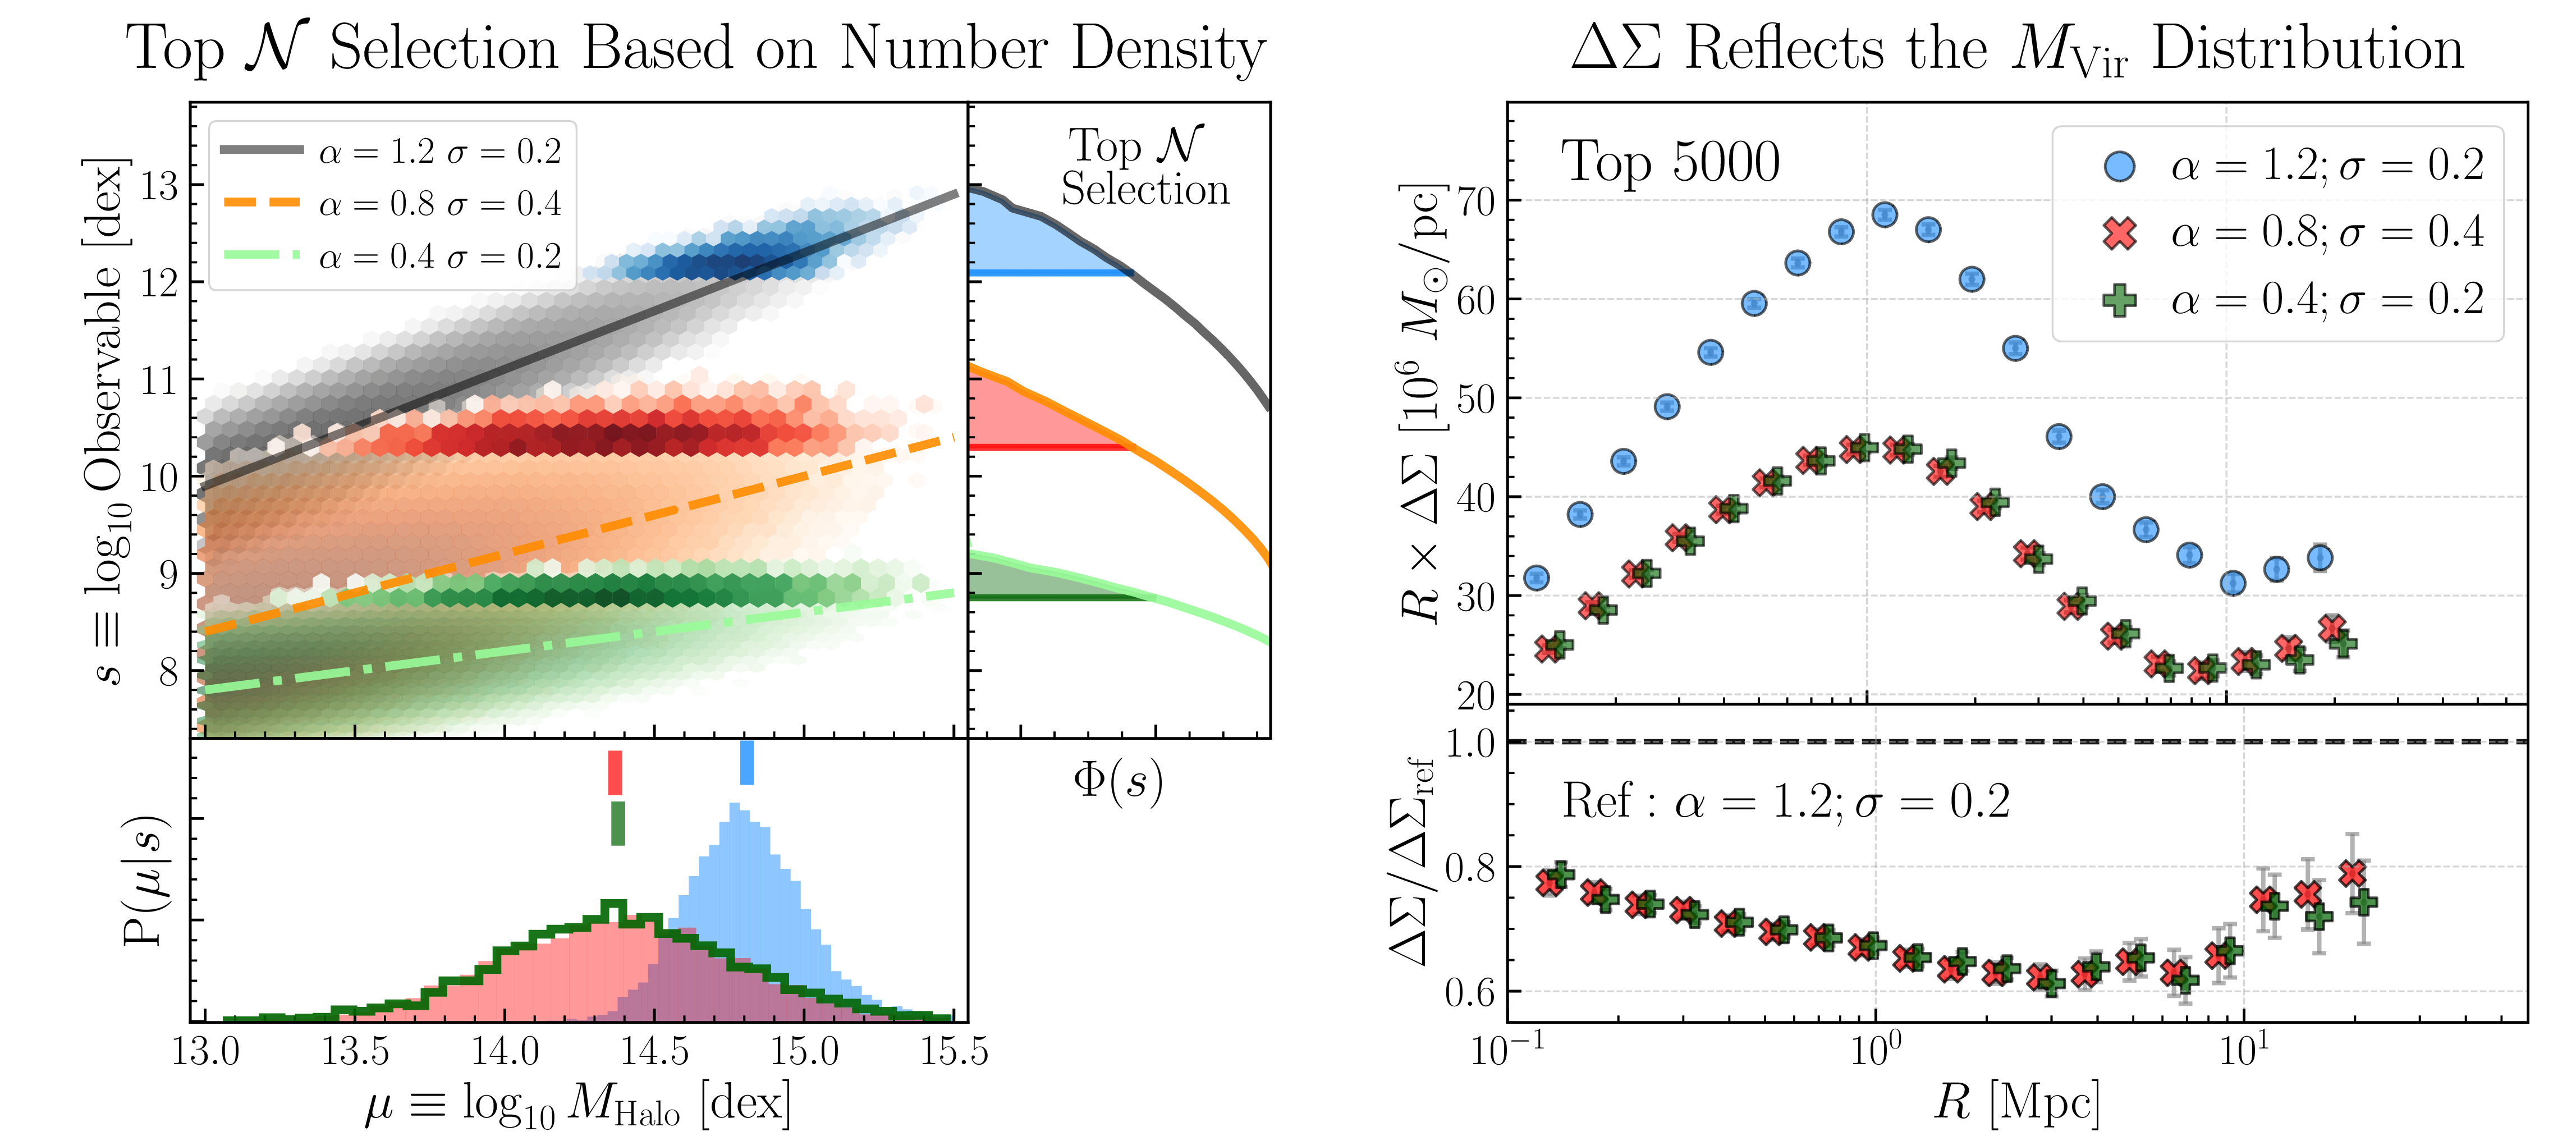
\includegraphics[width=\textwidth]{figure/topn_fig_1}
    \caption{
        \textbf{Left}:
            Demonstration of the \topn{} experiment: For the same set of halos sampled from the
            \mdpl2{} halo mass function, we mock the distributions of two hypothetical observables
            that follow \mhalo{}-observable relations with different slopes and scatters
            (blue v.s. orange shaded regions).
            We then select the top $N$ objects using the two observables and highlight them using
            scatter plots with the corresponding color.
            The $N$ value translates into a fixed volume number density threshold shown on the
            right sub-panel using the number density distributions of the two observables.
            On the bottom sub-panel, we can see that the same \topn{} selection results in
            different \mhalo{} distributions with different mean values (labeled by the short
            vertical bar) and scatters. 
            In this case, the \mhalo{}-observable relation with shallower slope and larger scatter
            (orange one) lead to lower average \mhalo{} and wider \mhalo{} distribution in the same
            \topn{} bin.
        \textbf{Right}:
            We show the stacked lensing signals of these two \topn{}-selected samples.
            We use the \rdsigma{} profile to highlight the scale-dependent differences between them.
            We also highlight the ratio of these two profiles in the bottom sub-panel.
            Such comparison reflects the difference of the underlying distributions of \mhalo{}
            (and potentially other halo properties) of the \topn{}-selected samples.
        }
        \label{fig:theory_1}
    \end{figure*}
%% ---------------------------------------------------------------------------------------------- %%

%% ---------------------------------------------------------------------------------------------- %%
%% Key Methods used in this work
%% ---------------------------------------------------------------------------------------------- %%

\section{Methodology and Modeling Framework}
    \label{sec:method}

    In this section, we outline the methodology to evaluate different possible \mvir{}
    proxies using high-quality galaxy-galaxy lensing data.
    We explain the basic idea of the \topn{} tests in \S \ref{sec:topn_intro}.
    In \S \ref{sec:model}, we explain the connection between the \sigmh{} at
    fixed observable value and the amplitude of the \dsigma{} profile.

%% ---------------------------------------------------------------------------------------------- %%
%% Philosophy of the Top N test
%% ---------------------------------------------------------------------------------------------- %%
\subsection{Philosophy of the \topn{} Test}
    \label{sec:topn_intro}

    The \topn{} test's philosophy is straightforward: to compare the \dsigma{}
    profiles of samples of galaxies (halos) selected using different \mvir{} proxies but with
    the same number density thresholds.
    Halo mass proxies, whose scaling relations with \mvir{} show either steeper slope or
    reduced scatter, will yield a higher lensing amplitude.
    For example, we can compare the stacked \dsigma{} profile of galaxies with
    the top 100 (or 100-500) most massive \mstar{} using \cmodel{} photometry to the profile
    of the top 100 (or 100-500) largest galaxies in size (at fixed volume). 
    The \topn{} essentially compares $\Delta\Sigma$ for samples in bins of fixed number density.

    Fig \ref{fig:theory_1} illustrates this main idea using two hypothetical observables with
    different \mvir{} scaling relations.
    In the same number density bin (e.g., top 5000 objects using each observable), the observable
    that correlates better with \mvir{} (blue) results in a \mvir{} distribution with higher
    average \mhalo{} and lower \sigmh{} value (left panel) and a stacked lensing profile with
    much higher amplitudes (right).
    \citet[][]{Reyes2008} applied a similar method to develop improved halo mass tracers
    of clusters.
    We should also point out that the ratio of \dsigma{} profiles often show scale dependent
    features which reveals subtle differences in other halo properties or large scale environment
    (right panel of Fig \ref{fig:theory_2}).
    This is another important application of the \topn{} strategy.

    Compared to sophisticated modeling strategy (e.g., \citealt{Sonnenfeld2019}), \topn{} test
    has the advantage of \emph{not} relying on detailed modeling of the lensing profile, which
    often has to ignore certain important systematics (e.g., off-center halo; baryonic effect,
    project effect).
    Not only \topn{} test can help us identify competitive \mvir{} proxy for ``cluster finding''
    (e.g., see \S \ref{sec:menvelope}), it can also reveal systematic differences between halos
    traced by different types of proxies (e.g. \mstar{} v.s richness;
    see \S \ref{sec:mstar_vs_richness}).

%% ---------------------------------------------------------------------------------------------- %%
%% Modeling Methodology
%% ---------------------------------------------------------------------------------------------- %%
\subsection{Modeling Methodology}
    \label{sec:model}

    To quantitatively interpret the differences of \dsigma{} profiles, we develop a simple
    method based on N-body simulations
    \mdpl2{}\footnote{\url{https://www.cosmosim.org/cms/simulations/mdpl2/}}
    and \smdpl{}\footnote{\url{https://www.cosmosim.org/cms/simulations/smdpl/}} and assumes a
    $\log$-linear \mvir{}-observable relation with constant Gaussian scatter.
    We estimate the $\sigma(M_{\rm vir} | {\rm Obs})$ value of a given \dsigma{} profile and
    infer the underlying \mvir{} distribution using this model.
    We explain the theoretical background of this method in \S \ref{sec:comp_scatters}, and
    describe its implementation in \S \ref{sec:estimate_scatter}.

%% ---------------------------------------------------------------------------------------------- %%
%% Figure: Theoretical exploration of the relations among scatters and its impact on
%%		   Delta Sigma profiles.
%% ---------------------------------------------------------------------------------------------- %%
    \begin{figure*}
    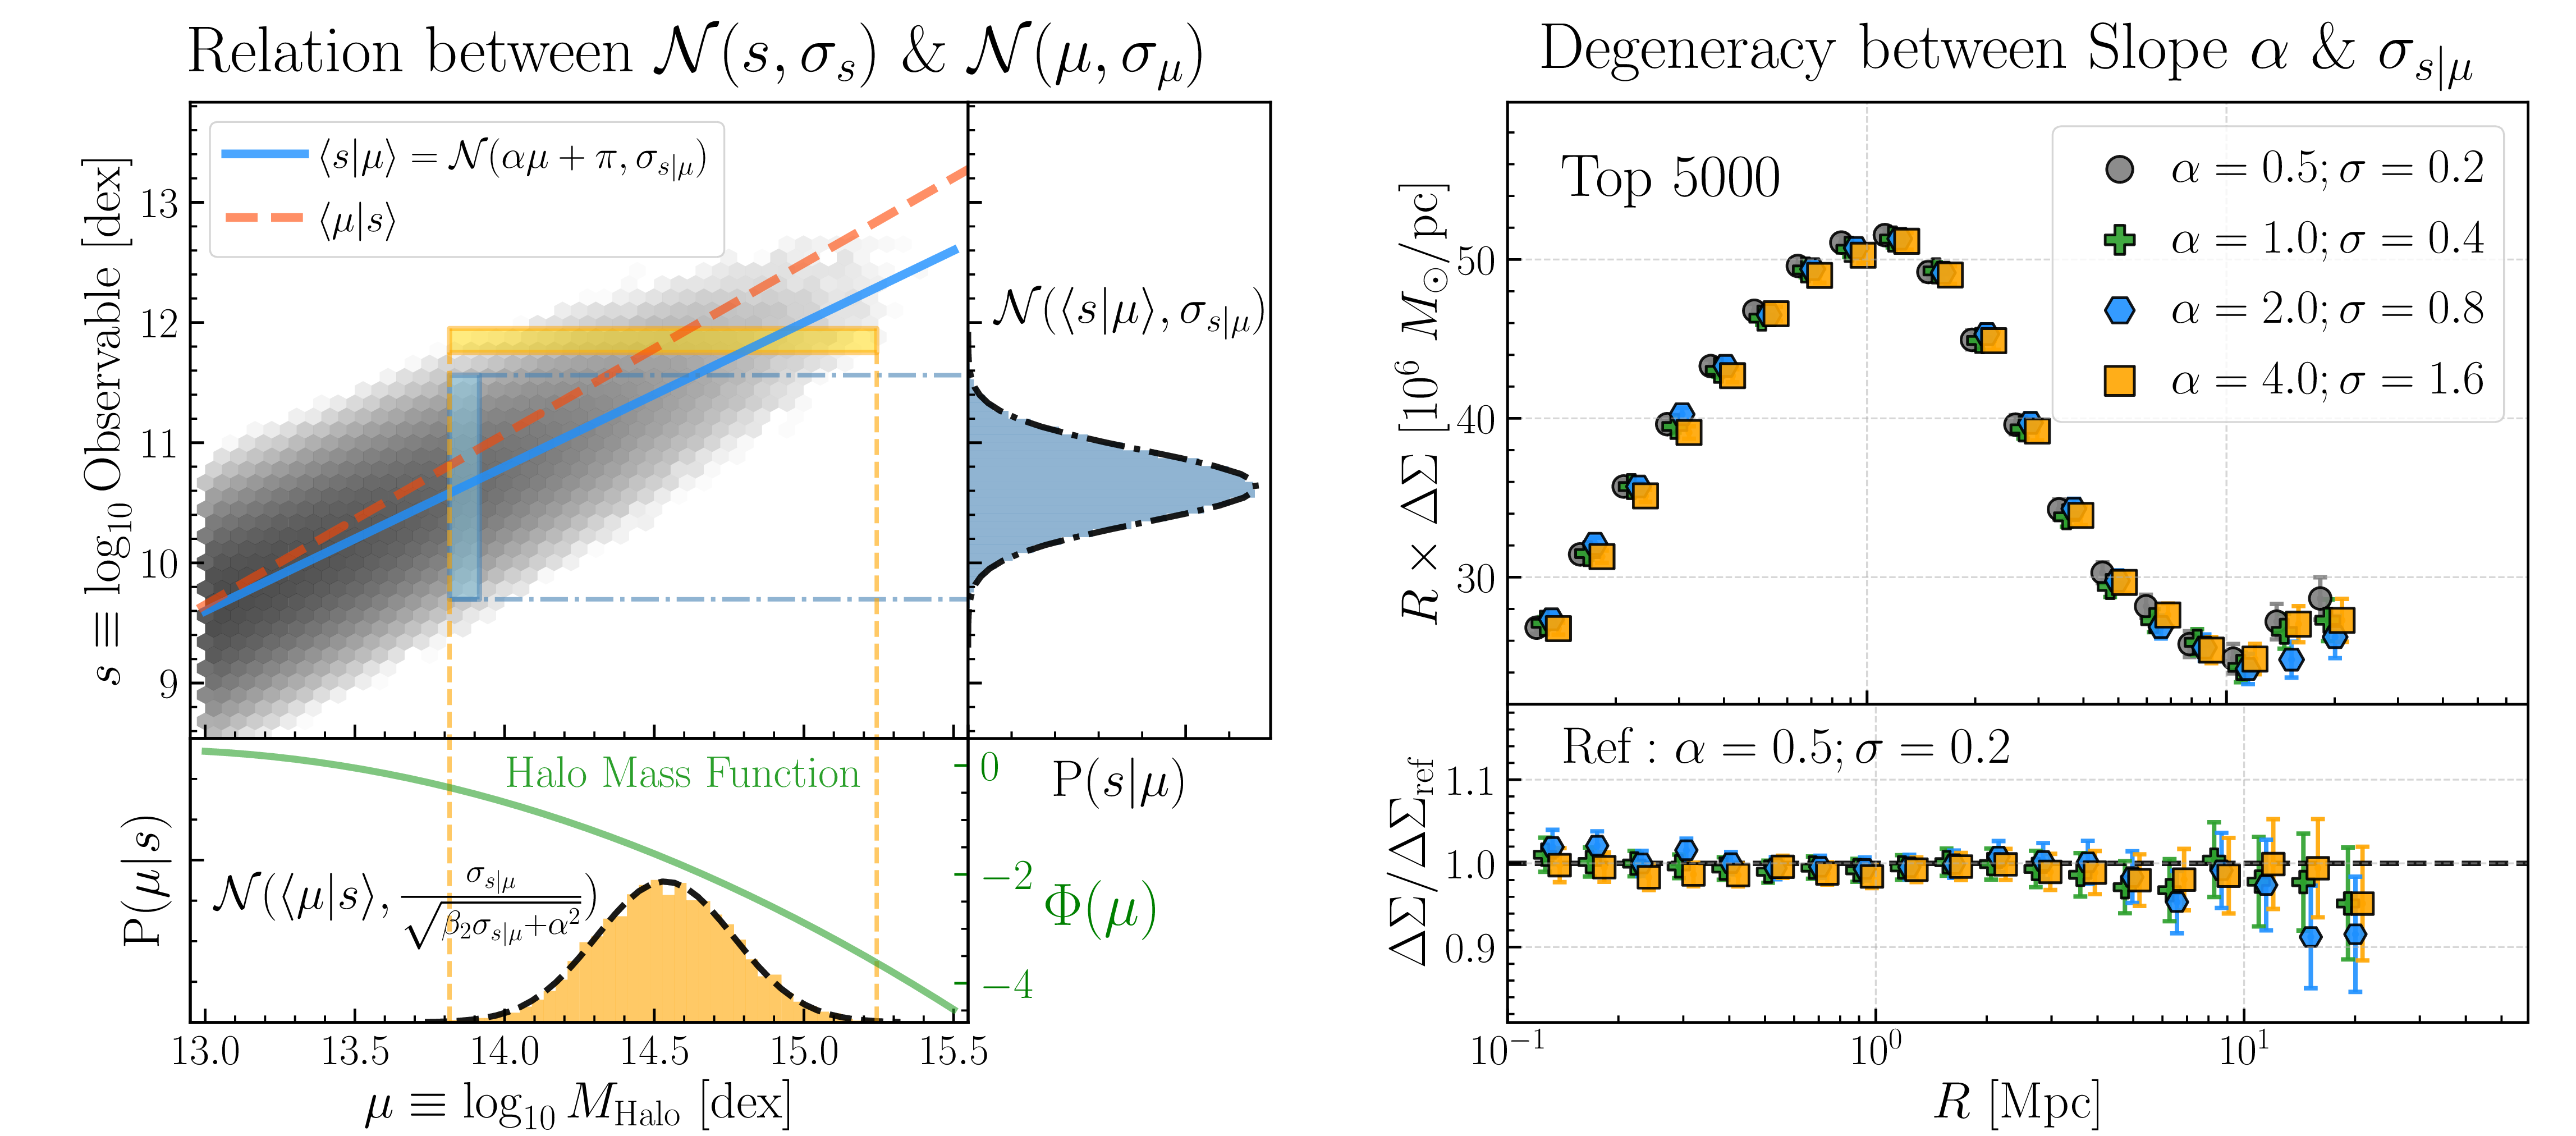
\includegraphics[width=\textwidth]{figure/topn_fig_2}
    \caption{
        \textbf{Left}:
            Using the \mhalo{} sampled from the \mdpl2{} halo mass function (HMF; green line in the
            bottom sub-panel), we show the distribution of a hypothetical observable, \obsSym{}, that
            relates to $\mu = \log(\Mhalo)$ by a linear relation with some scatter.
            By construction, the distribution of observable within a thin \mhalo{} bin (the blue
            rectangular region) $P(\obsSym | \mu)$ is a normal distribution around
            $\langle \obsSym | \mu \rangle = \alpha \mu + \pi$ with a scatter of
            $\sigma_{\obsSym | \mu}$(right panel, blue histogram).
            $P(\mu | \obsSym)$ (bottom panel, yellow histogram) is the distribution of \mhalo{} in
            a thin selection of \obsSym{} (yellow rectangular region), which can be well
            described by a normal distribution (black dashed-line) centered at the value given by
            Figure \ref{eq:mean_of_mu} with a scatter given by Figure \ref{eq:scatter_of_mu} that
            depends on $\sigma_{\obsSym | \mu}$, the slope of the \obsSym - $\mu$ relation, $\alpha$,
            and the curvature of the HMF, $\beta_2$.
            The gap between $\langle \obsSym | \mu \rangle$ and $\langle \mu | \obsSym \rangle$
            becomes smaller toward the lower \mhalo{} end as the slope of HMF becomes shallower.
        \textbf{Right}:
            In galaxy-galaxy lensing studies, we infer the average halo properties of a sample
            selected based on specific observable using the \emph{stacked} lensing profile.
            Observables with the same ratio $\alpha / \scatterObsSymMhalo$ have the same
            \scatterMhaloObsSym{} (see Figure \ref{eq:ratio_is_what_matters}) in the same volume
            number density bin, resulting in very similar \dsigma{} profiles.
            We highlight this degeneracy using the \rdsigma{} profiles of mock samples selected from
            four different scaling relations with the same $\alpha / \scatterObsSymMhalo$ and number
            density threshold.
            Using the first sample as the reference, we also show the ratios of \rdsigma{} profiles
            in the bottom sub-panel.
        }
        \label{fig:theory_2}
    \end{figure*}
%% ---------------------------------------------------------------------------------------------- %%

%% ---------------------------------------------------------------------------------------------- %%
%% Figure: DSigma profiles from MDPL2 and the impacts of scatter on DSigma profile and
%%         halo mass distribution
%% ---------------------------------------------------------------------------------------------- %%
    \begin{figure*}
        \centering
        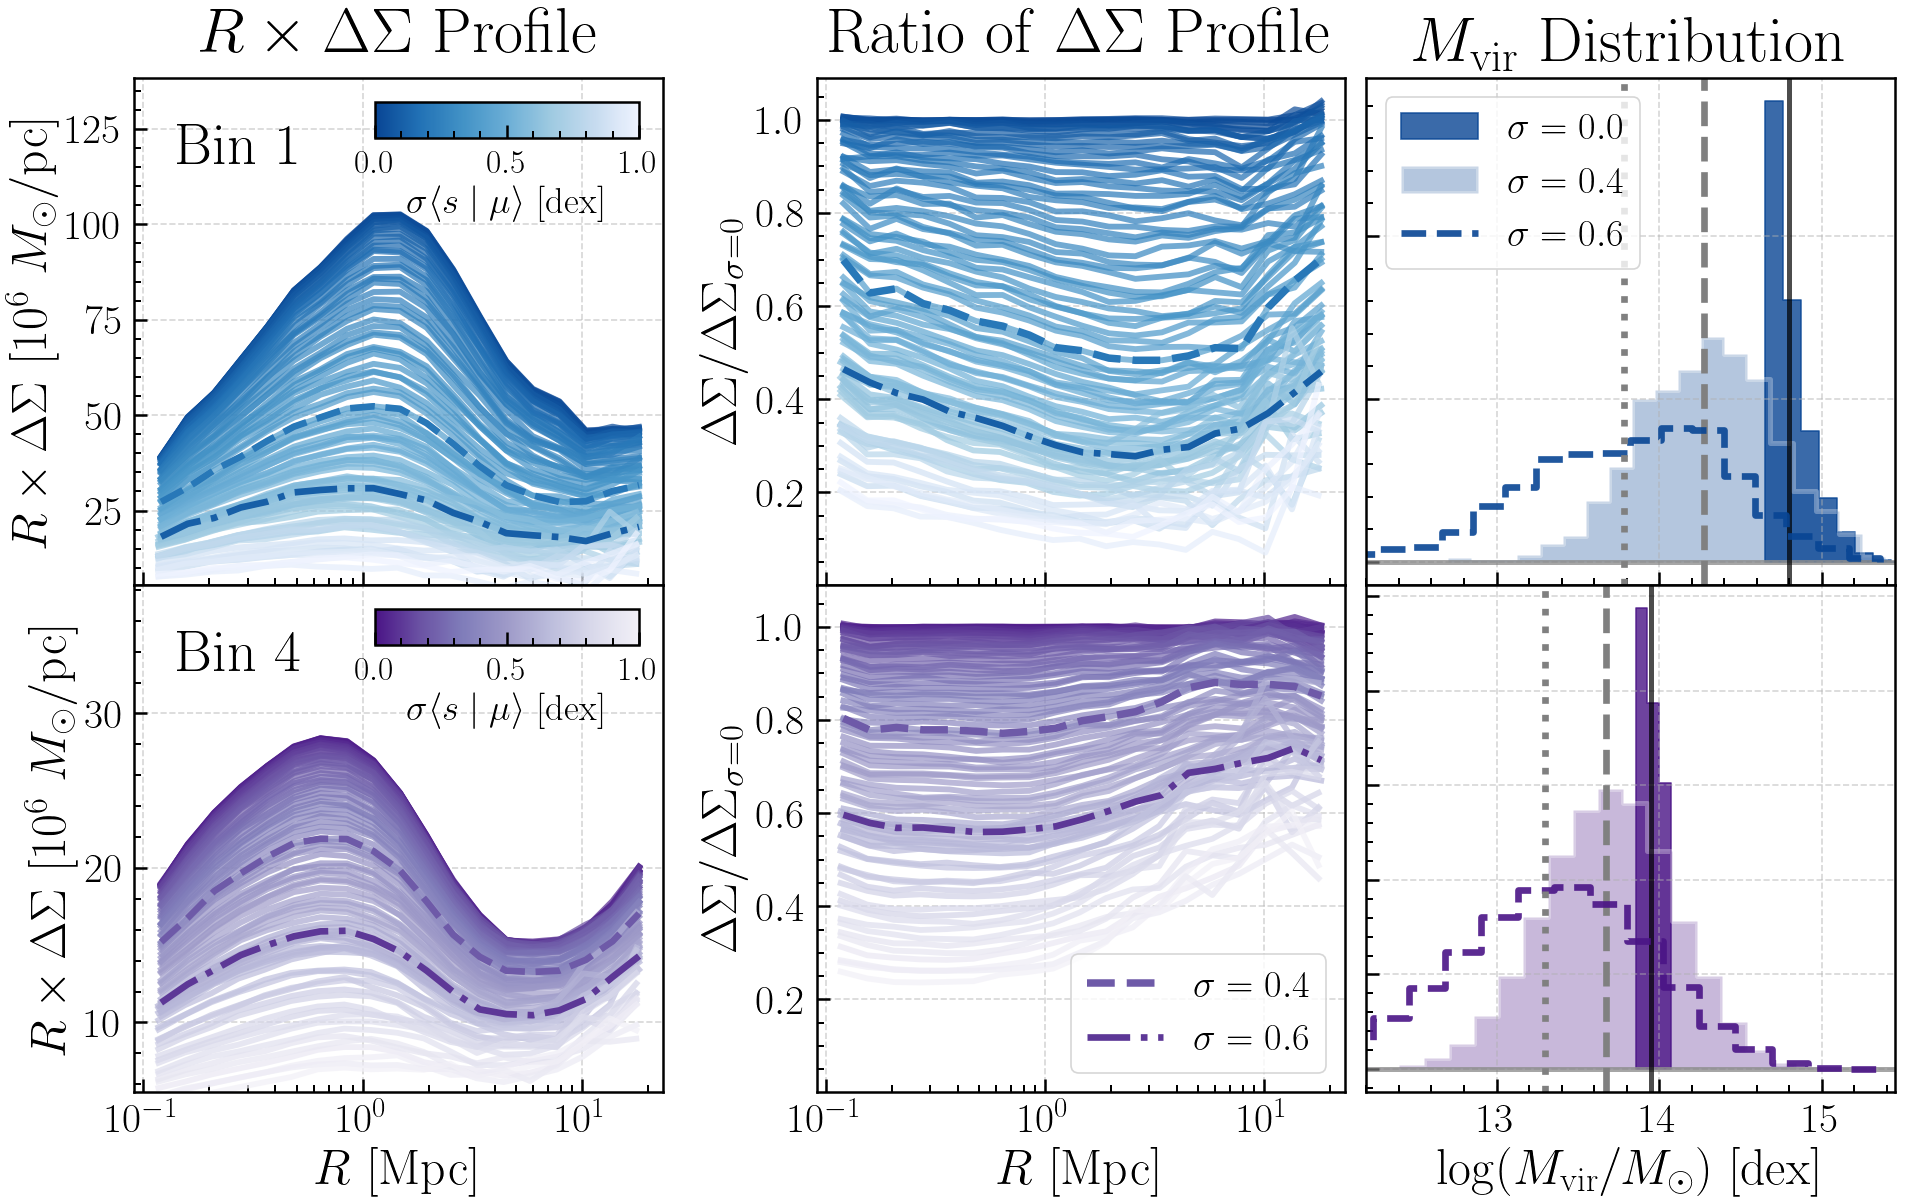
\includegraphics[width=16cm]{figure/topn_fig_5}
        \caption{
        We show the \dsigma{} profiles and \mhalo{} distributions of the \topn{} samples with
        a wide range of \mhalo{} scatters ($0<\sigma_{\langle s \mid \mu\rangle}<1$) using a
        combination of \mdpl2{} and \smdpl{} simulation.
        \textbf{Left}:
            The \rdsigma{} profiles of the \topn{} samples with different scatters of \mhalo{}.
            Colors reflect the scatter value. We highlight the profiles of the
            $\sigma_{\langle s \mid \mu\rangle}=0.4$ (dashed line) and $=0.6$ (dot-dashed line)
            samples.
        \textbf{Middle}:
            Similar to the left panels but showing the ratio between the \dsigma{} profiles of
            the \topn{} samples from non-zero $\sigma_{\langle s \mid \mu\rangle}$ scaling
            relation and the ``perfect'' sample ($\Delta\Sigma_{\sigma=0}$).
            We highlight the ratio for the $\sigma_{\langle s \mid \mu\rangle}=0.4$ and $=0.6$
            ones too.
        \textbf{Right}:
            We show the \mhalo{} distributions of the ``perfect'' \topn{} sample and the
            $\sigma_{\langle s \mid \mu\rangle}=0.4$ and $=0.6$ samples.
            We also label the mean \mhalo{} for each distribution.
        }
        \label{fig:mdpl2}
    \end{figure*}
%% ---------------------------------------------------------------------------------------------- %%

%% ---------------------------------------------------------------------------------------------- %%
%% Scaling relation and scatters
%% ---------------------------------------------------------------------------------------------- %%
\subsubsection{The relationship between \scatterMhaloObsSym{} and \scatterObsSymMhalo{}}
    \label{sec:comp_scatters}

    Assuming a generic observable that shows a $\log$-linear relation with the \mvir{} that shows
    a $\log$-normal scatter (e.g.,
    X-ray temperature \citealt{Lieu2016}, K-band luminosity \citealt{Ziparo2016}, and many others
    \citealt{Evrard2014, Farahi2018}), we explore the connection between the \sigmh{} of a sample
    and its observed \dsigma{} profile.

    The relationship between \obsSym{}$\equiv \log_{10}{\rm Observable}$ and
    $\mu \equiv \log_{10}M_{\rm Halo}$ depends on the halo mass function (HMF)
    \citep[\eg{}][]{Tinker2008}.
    Since we will focus on the high-\mhalo{} end of the HMF, we approximate the HMF using the
    following exponential functional form.

    \begin{equation}
        \hmf{} \equiv \frac{dn(\mu)}{d\mu{}}  = \exp \left(\beta_0 - \beta_1 \mu - \frac{\beta_2}{2} \mu^2 \right)
        \label{eq:quadratic_hmf}
    \end{equation}

    \noindent At the high-\mhalo{} end, HMF declines rapidly with \mhalo{} ($\beta_1 > 0$) with a
    steepening slope ($\beta_2 > 0$).

    We populate the halos with the generic observable using a $\log$-linear relation with a
    constant $\log$-normal scatter value.

    \begin{equation}
        \obsSym = \mathcal{N}(\slope \mu + \intercept,\ \scatterObsSymMhalo)
        \label{eq:lognormal_obs_given_mhalo}
    \end{equation}

    The scatter of observable at fixed \mhalo{}, \scatterObsSymMhalo{}, contains physical
    information about galaxy formation process and is the "scatter of SHMR" value most often
    quoted.
    Yet it is the scatter of \mhalo{} at fixed observable, \scatterMhaloObsSym{}, that really
    matters when selecting or ranking halos in observation.
    We briefly discuss the connection between \scatterObsSymMhalo{} and \scatterObsSymMhalo{}.
    Firstly, the probability density of the observable $\obsSym$ is,

    \begin{equation}
        P(\obsSym{}) \equiv \int_{0}^{\infty} \hmf{} P(\obsSym{} | \mu) d\mu
    \end{equation}

    At fixed \obsSym{} the scatter around the expected $\mu$,

    \begin{equation}
    \begin{aligned}
        \langle \mu | \obsSym \rangle
        &= \frac{1}{P(\obsSym)}
            \int_{0}^{\infty} \hmf{} P(\obsSym{} | \mu) \mu d\mu \\
        &= \frac{\left( \frac{\obsSym- \intercept}{\slope} - \beta_1 \left(\frac{\scatterObsSymMhalo}{\slope}\right)^2 \right)}{ 1 + \beta_2 \left(\frac{\scatterObsSymMhalo}{\slope}\right)^2}
        \label{eq:mean_of_mu}
    \end{aligned}
    \end{equation}

    \noindent The three components of $\langle \mu | \obsSym \rangle$ are:

    \begin{enumerate}

        \item The mean relation between the observable and halo mass, $(\obsSym- \intercept) /
        \slope$.

        \item A shift due to the Eddington bias caused by the linear slope of the HMF, $-\beta_1
        (\frac{\scatterObsSymMhalo}{\slope})^2$. In the case of $\beta_1 > 0$, this shift is to
        lower $\mu$ as there are more low $\mu$ objects that can be up-scattered into the
        selection than can be down-scattered.

        \item A second shift due to excess Eddington bias caused by the curvature of the HMF, $(1
        + \beta_2 (\frac{\scatterObsSymMhalo}{\slope})^2)^{-1}$. Again, $\beta_2 > 0$ results in
        more low $\mu$ objects and thus a shift to lower $\mu$.

    \end{enumerate}

    Similarly, the scatter in $\mu$ at fixed $\obsSym$,

    \begin{equation}
    \begin{aligned}
        \scatterMhaloObsSym{}
        &= \frac{1}{P(\obsSym{})}
            \int_{0}^{\infty} \hmf{} P(\obsSym{} | \mu) ( \mu  - \langle \mu \rangle )^2 d\mu \\
    	&= \frac{\scatterObsSymMhalo}{\sqrt{\beta_2 \scatterObsSymMhalo^2 + \slope^2}}
        \label{eq:scatter_of_mu}
    \end{aligned}
    \end{equation}

    \noindent which, in the case of a power law mass function ($\beta_2 = 0$), reduces to the
    commonly seen $\scatterObsSymMhalo / \slope$. The positive $\beta_2$ of the HMF decreases
    this scatter. Finally, higher moments such as the skewness or excess kurtosis confirm that
    $P(\mu | s)$ follows a Gaussian distribution.
    We summarize the above finding in the left panel of Figure \ref{fig:theory_2} where we
    simulate the HMF and the theoretical observable \obsSym{}.
    We show that the resulting distributions are consistent with the above discussion.

    Now, we rewrite Equation \ref{eq:scatter_of_mu} in a more practical form that makes it clear
    the dependence of \scatterMhaloObsSym{} is not on {\em both} \scatterObsSymMhalo{} and
    \slope, but rather the ratio of them.
    This is obvious in the case of a power law mass function ($\beta_2 = 0$) and is also true
    for the more general quadratic form (\ref{eq:quadratic_hmf}),

    \begin{equation}
        \scatterMhaloObsSym{}
        	= \frac{\scatterObsSymMhalo}{\sqrt{\beta_2 \scatterObsSymMhalo^2 + \slope^2}}
            = \left(\beta_2 + (\frac{\slope}{\scatterObsSymMhalo})^2\right)^{-1/2}
        \label{eq:ratio_is_what_matters}
    \end{equation}

    We demonstrate this in the right panel of Figure \ref{fig:theory_2}:
    we populate a simulation with observables that show a range of $\alpha$ and
    \scatterObsSymMhalo{}, but with the same ratio $\alpha / \scatterObsSymMhalo$.
    Under the same \topn{} selection, they show identical \dsigma{} profiles since they share the
    same \scatterMhaloObsSym{} value.


%% ---------------------------------------------------------------------------------------------- %%
%% Estimating scatter of halo mass
%% ---------------------------------------------------------------------------------------------- %%
\subsubsection{Estimating $\sigma(M_{\rm vir} | {\rm Obs})$}
    \label{sec:estimate_scatter}

    The discussion in \S\ref{sec:comp_scatters} demonstrates that we can compare the
    \scatterMhaloObsSym{} values of two \topn{} samples using their stacked \dsigma{} profiles:
    the sample selected by the ``better'' \mhalo{} tracer should show higher overall amplitude in
    its \dsigma{} profile.
    More importantly, now we can attempt to estimate the \scatterMhaloObsSym{} value from an
    observed \dsigma{} profile by comparing it to the \dsigma{} profile from simulation using the
    same number density selection.

    We start by populating the halos in simulations of observables that follow $log$-linear
    relations (Equation \ref{eq:lognormal_obs_given_mhalo}) with fixed slope value at $\alpha =
    1$ but with different \scatterObsSymMhalo{} values.
    In each of the realization, we derive the best-fit $\mu | \obsSym$ relation and estimate the
    \scatterMhaloObsSym{} value in pre-defined number density bins (\topn{} bins) used in
    observation.
    For each \topn{} bin, we calculate the stacked \dsigma{} profile and also store the
    underlying \mhalo{} distribution at different \scatterMhaloObsSym{} values.
    As the process of populating the halos is stochastic, we repeat this process both to improve
    the robustness of the predicted \dsigma{} profile, also to estimate the statistical
    uncertainty of the profile.
    After thoroughly searching through a large range of \scatterObsSymMhalo{} values, we can
    predict how does the stacked \dsigma{} profile vary with the scatter of \mhalo{} in each
    \topn{} bin on a densely sampled grid of \scatterMhaloObsSym{} values between 0.0 and 1.0
    dex.
    In the left columns of figure \ref{fig:mdpl2}, we show the predicted \dsigma{} profiles as a
    function of \scatterMhaloObsSym{} for the four \topn{} bins used in this work (defined in
    \S\ref{sec:binning}).
    In addition to the expected decreasing \dsigma{} amplitudes with increasing
    \scatterMhaloObsSym{} values, we also see scale dependent differences in the ratios of
    predicted \dsigma{} profiles.
    We highlight the \dsigma{} profiles with \scatterMhaloObsSym{}$=0.4$ and 0.6 dex along with
    their \mhalo{} distributions.
    In recent years, different modeling methods gradually converged to a
    \scatterObsSymMhalo{}$=0.2$ dex value for SHMR at high-\mhalo{} and low redshift (e.g.,
    \citealt{More2011, Leauthaud2012, Reddick2013, Behroozi2013, Tinker2017}).
    However, the slope of the SHMR suggests that the \scatterMhaloObsSym{} value should be
    considerably higher and in the $\sim 0.4$-0.6 dex range (e.g., Fig 5 \& 7 of
    \citealt{Wechsler2018}). Therefore it is essential to cover large \scatterMhaloObsSym{}
    values here.

    To estimate the best-fit \scatterMhaloObsSym{} value and its uncertainty of an observed
    \dsigma{} profile from certain \topn{} bin, we ``match'' it to the corresponding grid of
    predicted \dsigma{} profiles.
    For an observed lensing profile ($\Delta\Sigma_{\rm O}$) and its covariance matrix
    ($\boldsymbol{C}$), we define a straightforward $\chi^2$ value to evaluate how well does a
    given model profile ($\Delta\Sigma_{\rm M}$) describe the observed one

    \begin{equation}
        \chi^{2}=(\Delta\Sigma_{\rm M}-\Delta\Sigma_{\rm O})^{\top} \boldsymbol{C}^{-1}(\Delta\Sigma_{\rm M}-\Delta\Sigma_{\rm O})
        \label{eq:chi2}
    \end{equation}

    \noindent After calculating the $\chi^2$ value of every model \dsigma{} profile in a given
    \topn{} bin, we derive a $\chi^2$ curve that can help us derive the least-$\chi^2$
    \scatterMhaloObsSym{} value and its 1-$\sigma$ uncertainty range.
    We provide more detailed discussion of this procedure and a visualization in Appendix
    \ref{app:fitting}.

    We note that we combine the predictions from both \mdpl2{} and \smdpl{} simulations in the
    above process.
    Although \mdpl2{} has the large volume that helps us sample the very high-\mhalo{} end of
    HMF, it does not have the resolution to recover all the low-\mhalo{} halos required to model
    the \dsigma{} profile under high \scatterMhaloObsSym{} value.
    We use the \mdpl2{} simulation to cover the $0.00 <$\scatterMhaloObsSym{}$<0.65$ dex range
    with a 0.01 dex grid, and use \smdpl{} to cover the $0.65 <$\scatterMhaloObsSym{}$<1.0$ dex
    with a 0.02 dex grid size.
    Using the overlapping $\scatterMhaloObsSym{}$ range, we confirm the two simulations
    provide \dsigma{} profiles that are consistent within their statistical uncertainties.
    We use the $z=0.364$ snapshot from \mdpl2{} and the $z=0.404$ snapshot from \smdpl{}, which
    are the closest ones to the mean redshift ($\sim 0.4$) of the HSC sample.
    When comparing with observed \dsigma{} profiles, we do not modify the \dsigma{} from simulation 
    to account for the mis-centering or barynoic physics effect.
    We will explore the impacts of these systematics later.

    We should also point out that this model focuses on the underlying distribution of \mvir{},
    which is \emph{not} the only factor that impacts the \dsigma{} profile.
    We will briefly discuss this in \S \ref{sec:discussion} but want to emphasis here that
    \emph{the relative comparison of \scatterMhaloObsSym{} in the same \topn{} is more
    meaningful than the value itself.}
    In this work, it mainly serves as a way to evaluate the performance of different \mhalo{}
    proxies in the same number density bin.
    And to evaluate the impact of satellite galaxies on \dsigma{} profile, we also provide a
    special version of the model that can match the observed SMF and clustering signals of HSC
    massive galaxies.
    We provide more details of this model in Appendix \ref{app:hsc_model}.

%% ---------------------------------------------------------------------------------------------- %%
%% Figure: Definition of richness and number density bins.
%% ---------------------------------------------------------------------------------------------- %%
    \begin{figure*}
        \centering
        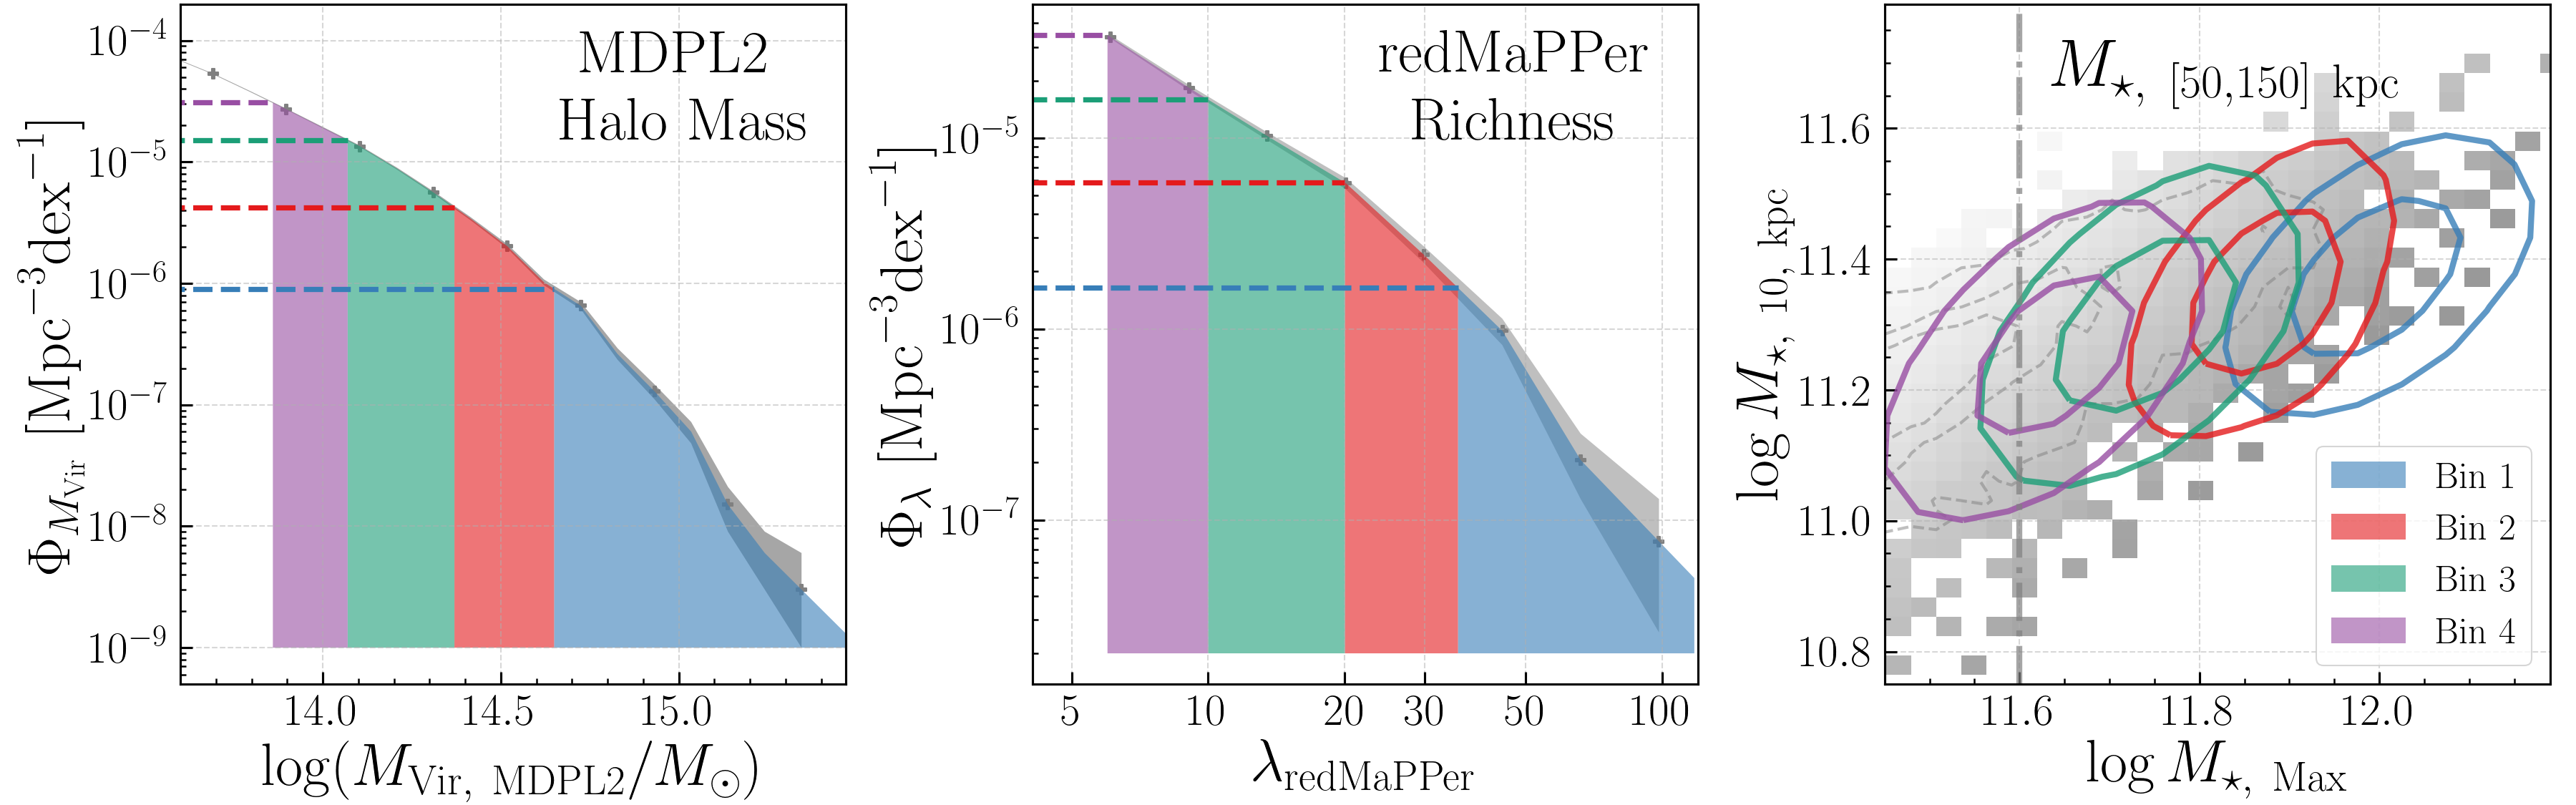
\includegraphics[width=16cm]{figure/topn_fig_4}
        \caption{
            \textbf{Top left}:
            The grey cross and the grey shaded region show the richness function of the
            \texttt{S16A} \redm{} clusters and its uncertainty from jackknife resampling.
            The four colored regions highlight the $\lambda_{\rm redMaPPer}$ ranges of the four
            \topn{} bins with the dashed-lines showing the number density boundary of each bin.
            \textbf{Top right}:
            Similarly, here, we show the HMF of the \mdpl2{} simulation and the \mhalo{} ranges
            of the four \topn{} bins.
            We can consider these \mhalo{} distributions as the ``perfect'' \topn{} selections
            when there is no scatter in the \mhalo{}-observable relation.
            \textbf{Bottom left}:
            The grey shaded region and the dashed-line contours show the distribution of HSC
            massive galaxies over the \mmax{}-\minn{} plane.
            The dot-dash line highlight \logmmax{}$=11.6$, a strict \mmax{} completeness
            limit.
            The four solid-line contours with corresponding colors highlight the distribution
            of massive galaxies in the four \topn{} bins when selecting using the \maper{150}
            aperture stellar mass.
            \textbf{Bottom right}:
            Here, we shows a similar plot but highlight the \topn{} samples selected using
            the outer envelope \mstar{} between 50 to 150 kpc (\menve{50}{150}) over the
            same \mmax{}-\minn{} plane.
            The distributions are visibly different with the \maper{150} ones.}
        \label{fig:density_bins}
    \end{figure*}
%% ---------------------------------------------------------------------------------------------- %%

%% ---------------------------------------------------------------------------------------------- %%
%% Section: Data and Sample Selection
%% ---------------------------------------------------------------------------------------------- %%
\section{Data}
    \label{sec:data}

    In this section, we introduce the imaging data  (\S \ref{sec:hsc}), the HSC massive
    galaxy sample (\S \ref{sec:galaxy_sample}), and the richness-selected galaxy cluster
    catalogs (\S \ref{sec:cluster_sample})

%% ---------------------------------------------------------------------------------------------- %%
%% HSC S16A data set
%% ---------------------------------------------------------------------------------------------- %%
\subsection{Hyper Suprime-Cam Survey Subaru Strategic Program}
    \label{sec:hsc}

    %% General information
    In this work, we use the $\sim 137$ \sqdeg{} of deep optical images from the \texttt{WIDE}
    layer of the \texttt{S16A} release of the Hyper Suprime-Cam Subaru Strategic Program
    (HSC-SSP, or HSC survey; e.g. \citealt{HSC-SSP, HSC-DR1, HSC-DR2})
    \footnote{\url{https://hsc.mtk.nao.ac.jp/ssp/}} - an ambitious cosmology survey using the
    8.2-m Subaru Telescope.
    HSC multi--band ($grizY$) images have impressive depth ($\sim$3--4 mag deeper than
    SDSS), superb seeing conditions (the mean $i$-band seeing has a $\sim 0.58$ arcsec Full-Width
    Half-Maximum , or FWHM), and fine pixel resolution (0.168 arcsec), all making this an ideal
    dataset to study galaxy structure and perform weak lensing measurements.

    We use the coadd images produced by \texttt{hscPipe 4.0.2}\footnote{
        \texttt{hscPipe} is a specifically modified version of the Large Synoptic Survey
        Telescope (LSST) pipeline (e.g.\ \citealt{Juric2015}; \citealt{Axelrod2010};
        {\url{https://pipelines.lsst.io}}) for HSC.
        The most recent version of \texttt{hscPipe} can be found here:
        \url{https://hsc.mtk.nao.ac.jp/pipedoc_e/}.
    }.
    Please see \citet{HSC-PIPE} for more details about the data reduction process and
    \citet{SynPipe} for its photometric performance.
    We also make use of the photometric redshift (photo-$z$) measurements of HSC galaxies from
    the \href{https://github.com/joshspeagle/frankenz}{\texttt{frankenz}}
    \citep{Speagle2019} algorithm. Please see \citet{HSC-PHOTOZ} for a summary of its
    performance.
    All galaxies and clusters used in this work are filtered through bright star masks
    (see \citealt{HSC-STAR} for details) to avoid contamination from saturated stars. Please
    refer to \citet{Huang2018b, Huang2018c, Huang2020} for a more thorough introduction to the
    HSC data.

    All the imaging data, along with the photometric and the photo-$z$ catalogs, has been released
    to the public\footnote{https://hsc.mtk.nao.ac.jp/ssp/data-release/}.
    In fact, the \texttt{PDR2} of the HSC survey already covers more area than the \texttt{S16A}
    data and has implemented several improvements in data reduction.
    Limited by the coverage of the available weak lensing shape catalog, we stick to the
    \texttt{S16A} data. To the best of our knowledge, new data releases will not change any of
    the main results.

%% ---------------------------------------------------------------------------------------------- %%
%% Massive Galaxy Sample
%% ---------------------------------------------------------------------------------------------- %%
\subsection{HSC Massive Galaxy Sample}
    \label{sec:galaxy_sample}

    Using the \texttt{S16A} data, we select a sample of massive galaxies at $0.19 < z <
    0.52$ for our analysis.
    In this redshift range, we can resolve the inner light profile ($r<10$ kpc) but also have the
    depth to explore the faint outskirts ($r \sim 100$ kpc).
    This is the same sample used in \citet{Huang2020}. Please refer to it for a detailed
    description. Here we only provide a brief summary.

    The sample contains 24926 massive galaxies made using a cut on the \texttt{CModel}-based \mstar{},
    $\mcmodel{} \geq 10^{11.2} M_{\odot}$.
    The \mcmodel{} is based on the \mlratio{} estimated by five-band SED fitting using
    \texttt{iSEDfit} (see \citealt{Moustakas2013}).
    All galaxies have valid 1-D surface brightness profiles measured in $i$-band with empirical
    background correction that enables non-parametric \mstar{} measurements out to $>100$ kpc.
    During the extraction of the 1-D profiles, $\sim 9$\% of the original sample was excluded due to
    contamination by nearby objects. We treat this as a small decrease of the effective survey
    area in this work.
    Among all 24926 galaxies, 15727 have a useful spec-$z$.
    However, when making a cut using the 100 kpc aperture \mstar{}, more than $90$\%
    of the 4765 galaxies with $\maper{100} \geq 10^{11.5} M_{\odot}$ have spec-z,
    as do all of the 2247 galaxies with $\maper{100} \geq 10^{11.6} M_{\odot}$.
    % When measured by the 100 kpc aperture \mstar{}, the 4765 galaxies with
    % $\maper{100} \geq 10^{11.5} M_{\odot}$ form a $>90$\% complete sample, and the
    % 2247 ones at \maper{100}$\geq 10^{11.6} M_{\odot}$ should be a \mstar{}-complete sample.

    Using similar samples of massive galaxies in HSC, we have uncovered remarkable structural
    diversity in the outer stellar halo (\citealt{Huang2018b}) and an interesting relation
    connecting the stellar mass distribution to the dark matter halo mass (\citealt{Huang2018c,
    Huang2020}).
    We have also compared the galaxy profiles with those in state-of-the-art hydro-simulations to
    gain insights into their assembly history (\citealt{Ardila2021}).
    We release the catalog of this massive galaxy sample here (\plan{Add URL}).

%% ---------------------------------------------------------------------------------------------- %%
%% Richness-based Galaxy Clusters
%% ---------------------------------------------------------------------------------------------- %%
\subsection{Red Sequence Cluster Catalogs}
    \label{sec:cluster_sample}

    Taking advantage of the well-defined ``red-sequence'' in low-$z$ galaxy clusters and
    the potential low-scatter nature of the \mvir{}-richness scaling relation
    (e.g., \citealt{Rozo2009, Rykoff2012}),
    richness-based cluster finders provide a promising way to identify massive halos in
    imaging data.
    % to explore cosmology and galaxy evolution.
    In this work, we test two ``red-sequence'' cluster catalogs.
    Here we briefly introduce the cluster samples. Please refer to the original references
    for technical details of the cluster finding algorithms.

%% ---------------------------------------------------------------------------------------------- %%
%% redMaPPer
%% ---------------------------------------------------------------------------------------------- %%
\subsubsection{\redm{} Clusters}
    \label{sec:cluster_redmapper}

    \redm{} \citet{Rykoff2014, Rozo2014, Rozo2015a, Rozo2015b}
    \footnote{\url{http://risa.stanford.edu/redmapper/}} is a popular cluster finding algorithm
    based on the richness of red-sequence galaxies.
    It has been applied to several large imaging surveys including SDSS (e.g.,
    \citealt{Rykoff2014}), DES (\citealt{Rykoff2016, McClintock2019}), and HSC.
    The \mvir{}--richness relation of \redm{} clusters has been investigated in multiple
    works (e.g., \citealt{Saro2015, Farahi2016, Simet2017, Melchior2017, Baxter2018, Murata2018,
    McClintock2019})

    We use an internal version of the \redm{} cluster catalog for \texttt{S16A} data
    (Kawinwanichakij \& Rykoff, private communication) based on the updated \texttt{Python}
    version of \redm{}\footnote{\url{https://github.com/erykoff/redmapper}}.
    The algorithm is similar to that used in \citet{Rykoff2016} with minor modifications.
    At $0.19 < z < 0.52$, the catalog contains 2784 clusters with $\lambda \geq 5$ and 249 with
    $\lambda \geq 20$.
    Of these clusters, 1837 have spec-$z$ (from a variety of sources) and the rest have a
    high-quality photo-$z$ from their red-sequence.
    The sample has a median photo-$z$ bias of $\delta_{z} \sim 0.0012$ (0.0009), a scatter of
    $\sigma_{z}/(1 + z) \sim 0.011$ (0.007), and a 4-$\sigma$ outlier fraction of $\sim 0.7$\%
    (0.5\%) for $\lambda \geq 5$ ($\geq 20$) clusters, showing performance consistent
    with that of the DES catalog \citet{McClintock2019}.
    We confirm that using the photo-$z$ from \redm{} does not affect relevant conclusions.
    Regarding the completeness of the cluster sample, \citet{McClintock2019} estimates that
    the DES limiting magnitude is deep enough for $0.2 L_{\star}$ galaxies at $z \sim 0.7$,
    and that the galaxy sample for \redm{} is $>90$-95\% complete.
    Given the deeper imaging in HSC, it is safe to expect even better completeness at
    $z<0.52$.

    In addition to the richness, \redm{} provides a list of candidates for the central galaxy
    along with their central probability ($P_{\rm cen}$).
    We choose the galaxy with the highest $P_{\rm cen}$ as the center of the cluster.
    Using a sub-sample of X-ray detected clusters, \citet{Zhang2019b} analyzes
    \redm{} mis-centering in DES for clusters with $\lambda > 20$. They find
    $\sim 83$\% of the clusters are well-centered.
    In the HSC \redm{} sample, 72\% (82\%) of clusters have central galaxies with $P_{\rm cen} >
    0.8$ (0.7).
    %Mis-centering will lead to under-estimated richness and will leave its impact in the
    % \dsigma{} profile of the cluster.

    We also test the 452 SDSS \texttt{DR8} \redm{} clusters (\citealt{Rykoff2014}) with
    $\lambda_{\rm SDSS} \geq 20$ in the \texttt{S16A} footprint.
    The SDSS sample is only complete at $z < 0.33$.

%% ---------------------------------------------------------------------------------------------- %%
%% CAMIRA
%% ---------------------------------------------------------------------------------------------- %%
\subsubsection{\camira{} Clusters}
    \label{sec:cluster_camira}

    \camira{}\footnote{\url{https://www.slac.stanford.edu/~oguri/cluster/}} is a
    red-sequence cluster finding algorithm developed by \citet{Oguri2014}.
    It has been applied to SDSS (\citealt{Oguri2014}) and HSC (\citealt{Oguri2018}) data.
    Unlike \redm{}, \camira{} does not have a richness-dependent radius, and instead counts
    red galaxies with $L \geq 0.2L_{\star}$ within a fixed $R\leq 1 h^{-1}$ Mpc.
    Its \mvir{}-richness relation has been calibrated using a variety of methods in
    \citet{Murata2019, Chiu2020a, Chiu2020b}.

    Here we use the public \texttt{S16A} \camira{} catalog that contains 1314 (338) clusters
    with $N_{\rm Mem} \geq 10$ ($\geq 20$) for $0.19 < z < 0.52$.
    We collect spec-$z$ measurements for 932 of these clusters.
    Our \camira{} sample has a median photo-$z$ bias of $\delta_{z} \sim -0.0041$ ($-0.0043$), a
    scatter of $\sigma_{z}/(1 + z) \sim 0.012$ (0.008), and a 4-$\sigma$ outlier fraction of
    $\sim 1.4$\% (0.7\%) for the $N_{\rm Mem} \geq 10$ ($\geq 20$) clusters.
    Similar to \redm{}, using the photo-$z$ has no impact on any key results.
    The \camira{} catalog shows excellent completeness when compared to X-ray clusters
    ($\gtrapprox 0.8$; see \citealt{Oguri2018} \S 5.3) or mock galaxy catalogs ($> 0.8$ for
    $M_{200c} > 5 \times 10^{13} h^{-1} M_{\odot}$ clusters at $0.3 < z < 0.6$; see
    \citealt{Oguri2018} \S 6).

    \camira{} assigns a central galaxy to each cluster without providing a central probability.
    \citet{Oguri2018} investigated the off-center distance ($R_{\rm off}$) distribution using
    matched X-ray clusters.
    While the distribution centered at $R_{\rm off} \approx 0.0$ Mpc, $\sim 30$\% of the clusters
    are offset from the X-ray peak with their $R_{\rm off}$ distribution described by a
    $\sigma=0.26 \pm 0.04 h^{-1}$ Mpc Gaussian component.

    We also test the clusters from the internal \texttt{S18A}, \texttt{S19A}, and
    \texttt{S20A} \camira{} catalogs that are in the \texttt{S16A} footprint.
    Differences in the data reduction process (e.g., background subtraction, deblending)
    can cause subtle differences in the cluster detection and richness measurements.
    However, we verify that these updates do not change any conclusions in this work.

%% ---------------------------------------------------------------------------------------------- %%
%% Key Measurements
%% ---------------------------------------------------------------------------------------------- %%
\section{Measurements}
    \label{sec:measure}

    Here we briefly introduce the methodologies behind the key measurements used in the \topn{}
    tests: the 1-D surface stellar mass density profiles ($\mu_{\star}$ \S \ref{sec:1d_prof}) and
    the galaxy-galaxy lensing \dsigma{} profiles (\ref{sec:dsigma}).

%% ---------------------------------------------------------------------------------------------- %%
%% 1-D Surface Mass Density Profiles
%% ---------------------------------------------------------------------------------------------- %%
\subsection{1-D Surface Mass Density Profiles}
    \label{sec:1d_prof}

    We have thoroughly discussed the method for extracting 1-D $\mu_{\star}$ profiles in
    \citet{Huang2018b, Huang2018c, Ardila2021}.
    We refer readers there for full technical details and provide a brief summary here.

    Using the \ellipse{} isophotal analysis function from \iraf{}, we extract 1-D $i$-band
    surface brightness profiles after aggressively masking out nearby contaminations and
    empirically correcting for the local background.
    In addition to the mask, the strategy of taking the median of flux density values along
    the isophote after 3-$\sigma$ clipping makes our 1-D profile robust against the high
    density of faint objects around massive galaxies (\citealt{Ardila2021}).
    With background subtraction, the 1-D profile is stable above $\sim 28$ \sb{},
    roughly corresponding to $r\sim 100$ kpc for our sample.
    The inner $\sim 5$-6 kpc of the profile is smeared by the seeing.

    We then convert the $i$-band surface brightness profile to the $\mu_{\star}$ profile using the
    average $i$-band \mlratio{} derived from SED fitting after applying corrections for
    galactic extinction and cosmological dimming.
    We ignore the \mlratio{} gradient in this work.
    Low-$z$ massive galaxies have shallow but negative color gradients
    (e.g., \citealt{Huang2018b, Wang2019, Montes2021}), which suggests
    the average \mlratio{} will underestimate the \mstar{} in the central region
    and overestimate it in the outskirts.
    However, the lack of clear dependence of color gradients on \mstar{} (\citealt{Huang2018b})
    suggests this systematic will not influence the conclusions of this work.
    The 1-D $\mu_{\star}$ profiles can be found \plan{here; ADD URL}

%% ---------------------------------------------------------------------------------------------- %%
%% Weak lensing measurements
%% ---------------------------------------------------------------------------------------------- %%
\subsection{Galaxy-Galaxy Lensing Measurements}
    \label{sec:dsigma}

    The galaxy-galaxy (g-g) lensing measurements done here follow almost exactly those in \citet{Speagle2019} and
    \citet{Huang2020}, which are themselves based on the methodology presented in \citet{Leauthaud2017}.
    This method subtracts lensing signals around a large number of random positions to achieve
    unbiased measurements (\citealt{Singh2017}).
    We put the equations to derive the \dsigma{} profile in Appendix \ref{app:dsigma_detail}.
    Compared to these earlier works, we provide a new recipe for the $f_{\rm bias}$ factor that
    accounts for the photo-$z$ dilution effect more accurately (see Equation
    \ref{eq:fbias})\footnote{ The typical $f_{\rm bias}$ factor value is around $\sim 1$-2\%
    level, and has no impact on the results of this work.}.

    We measure \dsigma{} in 11 physical radial bins that span from 200 kpc to 10 Mpc uniformly
    in $\log_{10}$ space.
    We use the public shape catalog for \texttt{S16A}\footnote{The shape catalog and other weak
    lensing data product can be found here:
    \href{here}{https://hsc-release.mtk.nao.ac.jp/doc/index.php/s16a-shape-catalog-pdr2}}
    based on the $i$-band coadd images and the re-Gaussianization algorithm
    (\citealt{HirataSeljak2003}).
    This is the same catalog used in the HSC Y1 cosmology results (e.g., \citealt{Hikage2019,
    Hamana2020}) and other cluster lensing analysis (e.g., \citealt{Umetsu2020}).
    Please see \citet{HSC-PIPE}, \citet{HSC-WLCAT}, and \citet{HSC-WLCALIB} for details about
    the shape measurements and lensing calibration.

    We adopt the \texttt{frankenz} photo-$z$ for source galaxies. 
    For the photo-$z$ quality cut, we use the ``basic'' cut ($\chi^{2}_{5} < 6$) in \citet{Speagle2019} 
    that removes about 5\% of source galaxies with unreliable photo-$z$.
    Most of them are at very low redshift so will not contribute to the lensing signals in this work.
    The lens-source separation criteria are: $z_{\rm s} - z_{\rm L} \ge 0.1$ and
    $z_{\rm s} > z_{\rm L} + \sigma_{s,68}$, where $\sigma_{s,68}$ is the 1$\sigma$ uncertainty
    of the source photo-$z$.
    We confirm that other photo-$z$ quality cuts and slightly different lens-source separation
    criteria do not affect any results.

    We use both jackknife resampling in 40 pre-defined sub-regions and bootstrap resampling
    with 2000 iterations to estimate the covariance matrix and the uncertainties of the \dsigma{}
    profiles.
    The two methods lead to fully consistent results.

    We use \texttt{v2.0} of the \texttt{Python} g-g lensing code \texttt{dsigma}
    \footnote{Code is publicly available here: \url{https://github.com/johannesulf/dsigma}} to
    calculate \dsigma{} profiles, and we release the \dsigma{} measurements of the massive
    galaxies and clusters \plan{here. ADD URL}

%% ---------------------------------------------------------------------------------------------- %%
%% Introduction of different halo mass proxies
%% ---------------------------------------------------------------------------------------------- %%
\section{Halo Mass Proxies and Bins}
    \label{sec:proxies}

    In this section, we summarize the observables that we use as \mvir{} proxies in the \topn{} tests.
    These observables can be broadly grouped into \mstar{}- and richness-based ones.
    On the \mstar{} side, we include \mstar{} based on the default HSC photometry for extended
    objects (\S \ref{sec:mcmodel}), a series of \mstar{} measured from the 1-D $\mu_{\star}$
    profiles (\S \ref{sec:maper} \& \S \ref{sec:menvelope}), and a linear combination of
    different aperture \mstar{} (\S \ref{sec:masap}).
    The richness-based proxies use clusters from the \redm{} and \camira{} red-sequence cluster finders.

    Both \mstar{} and richness have a physical connection to the underlying \mvir{}.
    More massive dark matter halos on average host more sub-halos and hence have a higher richness of
    (red) satellite galaxies.
    Similarly, more massive halos tend to host more massive galaxies.
    Both SHMR and \mvir{}-richness relations are well-established scaling relations at
    the high-\mvir{} end using both observations and hydro-simulations (e.g., \addref{}).
    Therefore it is natural to use both as first-order proxies of \mvir{}.

    Having introduced the proxies, we describe our number density bins and show the estimated
    scatter by comparing to the model described in section \ref{sec:estimate_scatter}.

    In the results section (\ref{sec:result}) we analyze in detail a few interesting proxies,
    but the results and associated figures for all proxies are available
    \plan{here. Add URL}

\subsection{Proxies}
%= > these argument can go in the discussion section or in the introduction
 %   But, we want to point out that
 %   1) \mstar{} measurement of one galaxy is a more straightforward approach and has several
 %   appealing features. Observationaly, it is more ``cost effective''. And it also suffers less
 %   from systematic issues such as the projection effect (\addref{}).
 %   2) In recent years, increasingly deep imaging surveys make us aware of the importance of the
 %   faint stellar outskirt of massive galaxies (\addref{}).
 %   After accounting for the \mstar{} in these diffuse stellar component closely tied to the
 %   halo assembly, we could further improve the capability of using \mstar{} as a halo mass %proxy.

%% ---------------------------------------------------------------------------------------------- %%
%% CModel Stellar Mass
%% ---------------------------------------------------------------------------------------------- %%
\subsubsection{\cmodel{} stellar mass}
    \label{sec:mcmodel}

    \cmodel{} is the default photometric model for extended objects in both the SDSS and HSC surveys,
    and will continue to be used in future imaging surveys.
    \cmodel{} attempts to describe the 2-D flux distribution of all extended objects with a
    combination of an exponential and a de Vacouleurs component (e.g., \citealt{HSC-PIPE}).
    It is an efficient and flexible model that provides statistically robust color measurements
    down to very faint magnitude (e.g., \citealt{SynPipe}).
    However, it does not always provide accurate total flux measurements, especially for
    massive galaxies whose surface brightness profiles can not be described with the \cmodel{}
    assumptions.
    In both the SDSS and HSC surveys, \cmodel{} photometry significantly underestimates the
    flux in the extended outskirts of massive, early-type galaxies (e.g., \citealt{Bernardi2013,
    Huang2018b}).
    In addition to the intrinsic model limitations, systematics in critical steps in
    the data reduction process such as background subtraction and object deblending often
    interfere with \cmodel{} fitting, making it even more challenging to accurately recover the
    correct total flux.
    These issues becomes more pronounced for deep imaging surveys such as HSC.

    Despite these issues, as \cmodel{} is the default for extended objects in many imaging
    surveys it is worth testing using the \topn{} methodology. This will show the impact of its
    deficiencies in the study of the galaxy-halo connection at the massive end.

    We note that the \cmodel{} photometry used here is from HSC \texttt{S16A} and an old
    version of \hscpipe{} (\texttt{v4}).
    Although newer versions of \hscpipe{} include multiple improvements and modifications,
    they do not solve the aforementioned issues for massive galaxies\footnote{ For instance, in the
    {\tt S18A} data release, \hscpipe{} significantly improves the background subtraction around
    bright object. But the well preserved low surface brightness envelopes around massive
    galaxies make object deblending more challenging. Overall, we do not see an improvement in
    the performance of \cmodel{} photometry. }.

    \begin{itemize}
        \item The \cmodel{} stellar mass is labeled as \mcmodel{} here.
    \end{itemize}

%% ---------------------------------------------------------------------------------------------- %%
%% Aperture Stellar Mass
%% ---------------------------------------------------------------------------------------------- %%
\subsubsection{Aperture \mstar{} From The 1-D Profile}
    \label{sec:maper}

    In \citet{Huang2018b}, we showed that the \mstar{} within a 100 kpc aperture is a better estimate
    of the ``total'' \mstar{} of massive galaxies than \mcmodel{}. We also demonstrated in
    \citet{Huang2018c, Huang2020} that changing the aperture used to measure \mstar{} changes the
    \mstar{}--\mvir{} relation.
    Here, we measure \mstar{} in apertures of 10, 30, 50, 75, 100, and 150 kpc in
    our \topn{} tests and evaluate how each performs as an \mvir{} proxy.

    In practice, we integrate the 1-D $\mu_{\star}$ profile after accounting for the isophotal
    shape of the galaxy to get the ``curve-of-growth'' (CoG) of \mstar{}, which describes the relation
    between the semi-major axis length of an elliptical aperture and the \mstar{} enclosed.
    Interpolation of the CoG provides the measurements of different aperture \mstar{}.
    We note that the $\mu_{\star}$ profile outside 100 kpc becomes less reliable due to background
    subtraction issues which affects the accuracy of aperture \mstar{} using larger radii.
    However, there does not appear to be much mass beyond 100 kpc.
    For our sample, the mean difference between \mstar{} within 150 and 100 kpc is only
    $\sim 0.02$ dex while the maximum difference is $\sim 0.15$ dex.

    The true $\mu_{\star}$ of massive galaxies certainly extends beyond the HSC surface
    brightness limit for individual galaxies (e.g., \citealt{Wang2019, Zhang2019, Montes2021,
    Kluge2021}). As a result, even the largest aperture \mstar{} we can measure is not the true total \mstar{}.
    We attempt to account for the ``missing \mstar{}'' by fitting a 1-D \ser{} model to the
    $\mu_{\star}$ profile between 50 and 100 kpc. We use this model to predict the mass well beyond
    the regime in which it can be measured.
    However, this model (assuming it correctly predicts the true profile) confirms that
    there is little mass beyond 100 kpc.
    The average difference between the \mstar{} in 300 and 100 kpc apertures is only $\sim\,0.05$ dex.

    Using the CoG we also measure the radius that contains 50\%, 80\%, and 90\% of the maximum
    \mstar{} measured by the 1-D profile (\mmax{}).
    We denote these radii as $R_{50}, R_{80}, R_{90}$.
    The ``half-mass'' or effective radius ($R_{50}$) provides another way to define apertures
    in addition to the physical size.
    For example, we can measure \mstar{} out to $2\times R_{50}$ or $4\times R_{50}$.
    We briefly explore the result of using these radius based proxies Appendix
    \ref{app:size}.

    \begin{itemize}
        \item Aperture masses using physical sizes are labeled as \maper{10}, \maper{100},
        \maper{300}.

        \item Aperture masses using $R_{50}$ are labeled as $M_{\star,\ 2R_{50}}$, $M_{\star,\
           4R_{50}}$.
    \end{itemize}

%% ---------------------------------------------------------------------------------------------- %%
%% Outer Envelope Stellar Mass
%% ---------------------------------------------------------------------------------------------- %%
\subsubsection{Outer Envelope \mstar{}}
    \label{sec:menvelope}

    In \citet{Bradshaw2020}, the authors noticed that the ``\exsitu{}'' component
    (the stellar mass that formed outside the halo of the main progenitor)
    of massive galaxies seems to have a tighter relation with \mvir{} than either the ``\insitu{}'' component
    or the total \mstar{}.
    This is also consistent with the modeling results from \citet{Huang2020}.

    While we cannot separate the \exsitu{} component from the \mstar{} distribution,
    recent simulations and observations suggest that the \exsitu{} stars dominate the
    outskirts of massive galaxies (\addref{}).
    It is therefore interesting to test whether the outer envelope \mstar{} is a useful \mvir{}
    proxy using the \topn{} tests.

    Here we simply define this ``outer envelope'' \mstar{} as the difference between
    two aperture \mstar{}.
    For example, the \mstar{} between 50 and 100 kpc, or between $2 \times R_{50}$ and
    $4 \times R_{50}$.
    It is not obvious which combination of radial boundaries will provide the best
    \exsitu{} \mstar{} proxy, so we explore a range of different definitions of the
    outer envelope.

    We should mention that many of the massive galaxies here are the central galaxies
    (or the brightest cluster galaxy, BCG) of galaxy cluster. 
    Their ``outer envelope'' is commonly known as the Intra-Cluster Light (ICL).
    We avoid that terminology because:
    1) the photometric definition of ICL is often ambiguous and arbitrary (e.g.,
    \citealt{Kluge2021})
    2) not all massive galaxies in our sample live in the
    center of cluster-level halos (i.e., \mvir{}$\geq 10^{14} M_{\odot}$).
    Therefore we prefer to use the more general term -- outer envelope -- to describe the
    outer structure of all massive galaxies.
    
    Also, when estimating the outer envelope mass from 1-D surface brightness profile,
    we assume fixed \mlratio{} value and isophotal shape that represent the inner region
    better.
    These low-$z$ massive galaxies on average show shallow negative optical color
    (hence \mlratio{}) and axis ratio gradients. 
    In our case, the color gradient means we could slightly over-estimate the outer envelope
    stellar mass while the axis ratio gradient can lead to under-estimation.
    We ignore these minor systematics here and will look into more accurate outer envelope 
    \mstar{} measurement later.
    We also perform \topn{} test using the luminosity of the outskirt and see no 
    change in key results.

    \begin{itemize}
        \item Outer envelope \mstar{} are represented as \menve{10}{100}, \menve{50}{100}, or
        $M_{\star,\ [2,4]R_{50}}$ in this work.

    \end{itemize}

%% ---------------------------------------------------------------------------------------------- %%
%% Halo mass based on ASAP model
%% ---------------------------------------------------------------------------------------------- %%
\subsubsection{\asap{} model}
    \label{sec:masap}

    In \citet{Huang2020}, we presented a phenomenological model (\asap{}) that connects a linear
    combination of \maper{10} and \maper{100} to the \mvir{} of the host halo of massive galaxies
    (\maper{100}{}$\geq 10^{11.5} M_{\odot}$).
    We constrained this model using the SMFs for \maper{10} and \maper{100} along with the
    \dsigma{} profiles of galaxies in 12 2-D bins over the \maper{100}-\maper{10} plane.
    In \citet{Ardila2021}, we provided an updated \asap{} recipe to predict \mvir{} of a
    massive galaxy based on its \maper{100} and \maper{10}:

    \begin{equation}
        \begin{aligned}
        \log M_{\mathrm{vir}} &=3.26 \times\left(\log M_{\star}^{100}-11.72\right) \\
        &-2.46 \times\left(\log M_{\star}^{10}-11.34\right) \\
        &+13.69
        \end{aligned}
        \label{eq:asap}
    \end{equation}

    While we have shown (\citealt{Huang2020}) that the \asap{} model predicts the
    {\em average} \mvir{} of clusters
    better than the simple SHMR model, here we investigate the scatter of this
    prediction for individual galaxies.

    \begin{itemize}

        \item We label this \mvir{} predicted by \asap{} model as \masap{}.

    \end{itemize}

%% ---------------------------------------------------------------------------------------------- %%
%% Halo mass proxies based on optical richness
%% ---------------------------------------------------------------------------------------------- %%
\subsubsection{Richness}
    \label{sec:proxy_richness}

    We compare these \mstar{}-based proxies to ones based on the richness derived by two popular
    red-sequence cluster finders: \redm{} and \camira{} (introduced in \S
    \ref{sec:cluster_redmapper} and \S \ref{sec:cluster_camira}).
    Calibrations of the \mvir{}--richness relations suggest that the richness of
    red-sequence galaxies is a very promising \mvir{} proxy (e.g., \addref{}).

    Theoretically speaking, richness should out-perform any \mstar{}-based \mvir{} proxy
    as the \mvir{}--richness relation has much steeper slope than the \mvir{}-\mstar{} relation
    (e.g., \addref{}).
    Supporting this theory, \mvir{}--richness calibration works also often report very small
    scatter values at the high \mvir{} end (e.g., \addref{}).
    Therefore a \topn{} comparison between \mvir{}- and richness-based proxies can help us
    confirm this expectation, or reveal interesting complexities.

    \begin{itemize}

        \item For \redm{}, we label its richness measurement as $\lambda_{\rm redMaPPer}$.

        \item For \camira{}, we use $N_{\rm CAMIRA}$ to represent the richness measurement.

    \end{itemize}

%% ---------------------------------------------------------------------------------------------- %%
%% Design TopN bins
%% ---------------------------------------------------------------------------------------------- %%
\subsection{Number Density Bins}
    \label{sec:binning}

    To perform the \topn{} tests using the previously mentioned proxies, we design four number
    density bins based on the richness of HSC \redm{} clusters ($\lambda_{\rm redMaPPer}$).
    These four bins correspond to the $\lambda_{\rm redMaPPer}$ ranges of $[35, 100], [20, 35),
    [10, 20), [6, 10)$ and have 50, 197, 662, \& 1165 objects in each bin.
    We refer to these bins as Bin 1 (richest clusters) through to Bin 4 (least rich clusters).
    The total number (2074) of objects is slightly smaller than the number of \logmaper{100}$\geq
    11.6$ galaxies (2247), which defines a \mstar{}-complete sample.
    Limited by the small area covered by the \texttt{S16A} data, we unfortunately have to squeeze
    a large range of $\lambda_{\rm redMaPPer}$ in Bin 1 so that we have enough objects
    to generate a \dsigma{} profile with decent \snratio{}.

    Figure \ref{fig:density_bins} shows how these bins in $\lambda_{\rm redMaPPer}$ correspond to
    bins in number density (top-left panel) and halo mass, using the HMF from \mdpl2{}
    (top-right panel).
    In the perfect scenario, Bin 1, 2, \& 3 are well above the conventional standard for
    ``galaxy cluster'' (\logmvir{}$\geq 14.0$) while the mean \mvir{} of Bin 4 is on the boundary
    between a cluster and a ``massive group''.

    The $N_{\rm Mem} > 10$ threshold for the \camira{} clusters means it does not have enough
    objects for Bin 4, therefore we only consider the first three bins.
    Similarly, for the SDSS \redm{} catalog, we only include Bins 1 \& 2, and we note that the
    richness range for Bin 4 is challenging even for deep imaging surveys such as HSC.
    We must therefore take the results for \redm{} in Bin 4 with some caution.

    We were unable to measure \mstar{} for $\sim\,9$\% of galaxies due to excessive blending which
    prevented the extraction of a 1-D profile. This reduces the effective area and volume of this sample.
    We do not correct for this when selecting the \topn{} galaxies. The effect of this can
    only reduce the \dsigma{} amplitude, but we verify it does not affect our results.

    We summarize the key properties of these four bins in Table \ref{tab:summary}.


%% ---------------------------------------------------------------------------------------------- %%
%% Table.1: Summary for a few important halo mass proxies
%% ---------------------------------------------------------------------------------------------- %%
\begin{table*}
\resizebox{0.7\textwidth}{!}{%
\small
\begin{tabular}{|c|cccc|}
\hline
\rowcolor[HTML]{d8dcd6} Property   & Bin 1   & Bin 2   & Bin 3  & Bin 4 \\ \hhline{|=====|}

$N_{\rm Sample}$     &   50  &  197  &  662  &  1165  \\  

$\log_{10} M_{\rm vir,\ \rm MDPL2}$  & [14.66, 15.55] & [14.38, 14.66) & [14.08, 14.38) & [13.86, 14.08) \\

$n(>M_{\rm vir})$  & $5.11\times 10^{-7}$ & $2.52\times 10^{-6}$ & $9.29\times 10^{-6}$ & $2.12\times 10^{-5}$ \\ \hhline{|=====|}

\multirow{2}{*}{$\lambda_{\rm redMaPPer}$}  &  [35, 120] &  [20, 35)  & [10, 20) &  [6, 10)  \\
& \sigmvir{}$=0.27\pm0.02$ & $0.38\pm0.02$ & $0.39\pm0.02$ & $0.58\pm0.02$ \\ \hline
                                            
\multirow{2}{*}{$N_{\rm CAMIRA}$}  &  [35, 75) & [21, 35) & [12, 21) &  \\
& \sigmvir{}$=0.30\pm0.03$ & $0.36\pm0.01$ & $0.50\pm0.02$ & {} \\ \hhline{|=====|}

\multirow{2}{*}{$\log_{10} M_{\star, \rm CModel}$}   & [11.88, 12.19] & [11.77, 11.88) & [11.67, 11.77) & [11.60, 11.67) \\ 
& \sigmvir{}$=0.60\pm0.04$ & $0.64\pm0.04$ & $0.87\pm0.06$ & $0.82\pm0.03$ \\ \hline

\multirow{2}{*}{$\log_{10} M_{\star, 30\ \rm kpc}$} & [11.77, 12.00] & [11.69, 11.77) & [11.61, 11.70) & [11.53, 11.61) \\ 
& \sigmvir{}$=0.52\pm0.04$ & $0.57\pm0.03$ & $0.61\pm0.03$ & $0.61\pm0.02$ \\ \hline

\multirow{2}{*}{$\log_{10} M_{\star, 50\ \rm kpc}$} & [11.86, 12.10] & [11.76, 11.86) & [11.66, 11.76) & [11.58, 11.66) \\ 
& \sigmvir{}$=0.46\pm0.04$ & $0.53\pm0.03$ & $0.59\pm0.02$ & $0.61\pm0.02$ \\ \hline

\multirow{2}{*}{$\log_{10} M_{\star, 100\ \rm kpc}$} & [11.93, 12.18] & [11.83, 11.93) & [11.71, 11.83) & [11.63, 11.71) \\ 
& \sigmvir{}$=0.38\pm0.02$ & $0.51\pm0.02$ & $0.56\pm0.02$ & $0.60\pm0.02$ \\ \hline

\multirow{2}{*}{$\log_{10} M_{\star, 150\ \rm kpc}$} & [11.96, 12.21] & [11.85, 11.96) & [11.73, 11.85) & [11.64, 11.73)  \\ 
& \sigmvir{}$=0.37\pm0.03$ & $0.47\pm0.03$ & $0.56\pm0.02$ & $0.57\pm0.03$ \\ \hhline{|=====|}

\multirow{2}{*}{$\log_{10} M_{\star, [50, 100]}$} & [11.20, 11.60] & [11.00, 11.20) & [10.80, 11.00) & [10.63, 11.00)  \\ 
& \sigmvir{}$=0.36\pm0.02$ & $0.43\pm0.02$ & $0.44\pm0.02$ & $0.48\pm0.02$ \\ \hline

\multirow{2}{*}{$\log_{10} M_{\rm Vir,\ ASAP}$} & [14.45, 15.28] & [14.09, 14.45) & [13.80, 14.11) & [13.60, 13.80)  \\ 
& \sigmvir{}$=0.38\pm0.03$ & $0.44\pm0.02$ & $0.48\pm0.02$ & $0.56\pm0.02$ \\ \hline

\end{tabular}%
}
\caption{
	Summary of results from the \topn{} test results in four number density bins. 
	The first three rows summarize the basic properties of each bin.
	$N_{\rm sample}$ is the number of HSC galaxies in each bin. 
	$\log_{10}M_{\rm vir, MDPL2}$ shows the corresponding halo mass range in this number density bin
	based on the \mdpl2{} simulation. 
	This is the \mvir{} range for an ideal (zero scatter) \topn{} selection.
	$n(>M_{\rm Vir})$ is the volume number density of halos above the lower-\mvir{} threshold.
	Subsequent rows contain the key results for different halo mass proxies. 
	The first row shows the range of the observed properties in the four bins.  The second row shows
	the best--fit scatter of \mvir{} at fixed observable ($\sigma_{\mathcal{M}|\mathcal{O}}$) of
	\mvir{} in each bin along with its uncertainty.
	For a complete summary table of all the properties we tested, please see this \texttt{Jupyter} notebook \href{https://github.com/dr-guangtou/jianbing/blob/master/notebooks/topn_result_summary.ipynb}{\faGithub} 
	}
\label{tab:summary}
\end{table*}
%% ---------------------------------------------------------------------------------------------- %%

%% ---------------------------------------------------------------------------------------------- %%
%% Main Results
%% ---------------------------------------------------------------------------------------------- %%
\section{Results}
    \label{sec:result}

    We now present the main results.
    We first qualitatively evaluate the impact on \dsigma{} of satellite contamination when ranking
    by \mstar{} (\S \ref{sec:satellite}).
    Then we show the first set of key findings of the \topn{} test focusing on the {\em amplitude}
    and inferred \sigmh{} of various \mvir{} proxies (\S \ref{sec:topn_results}).
    We highlight the behaviors of \mcmodel{} (\S \ref{sec:m100_cmodel}) and the \mstar{} of the
    outskirts, \menve{50}{100} (\S \ref{sec:m100_outskirt})
    before summarizing the overall trends of \sigmh{} across the number density bins for a selection
    of \mvir{} proxies (\S \ref{sec:trend}).
    Finally, we compare the {\em shape} of the \dsigma{} profiles of the \mstar{}- and richness-selected
    halos and determine whether they are consistent with the pure scatter model or show other
    features (\S \ref{sec:mstar_vs_richness}).

%% ---------------------------------------------------------------------------------------------- %%
%% Figure: Impact of satellites on the M100kpc selected DSigma profiles
%% ---------------------------------------------------------------------------------------------- %%
  \begin{figure}
      \centering
      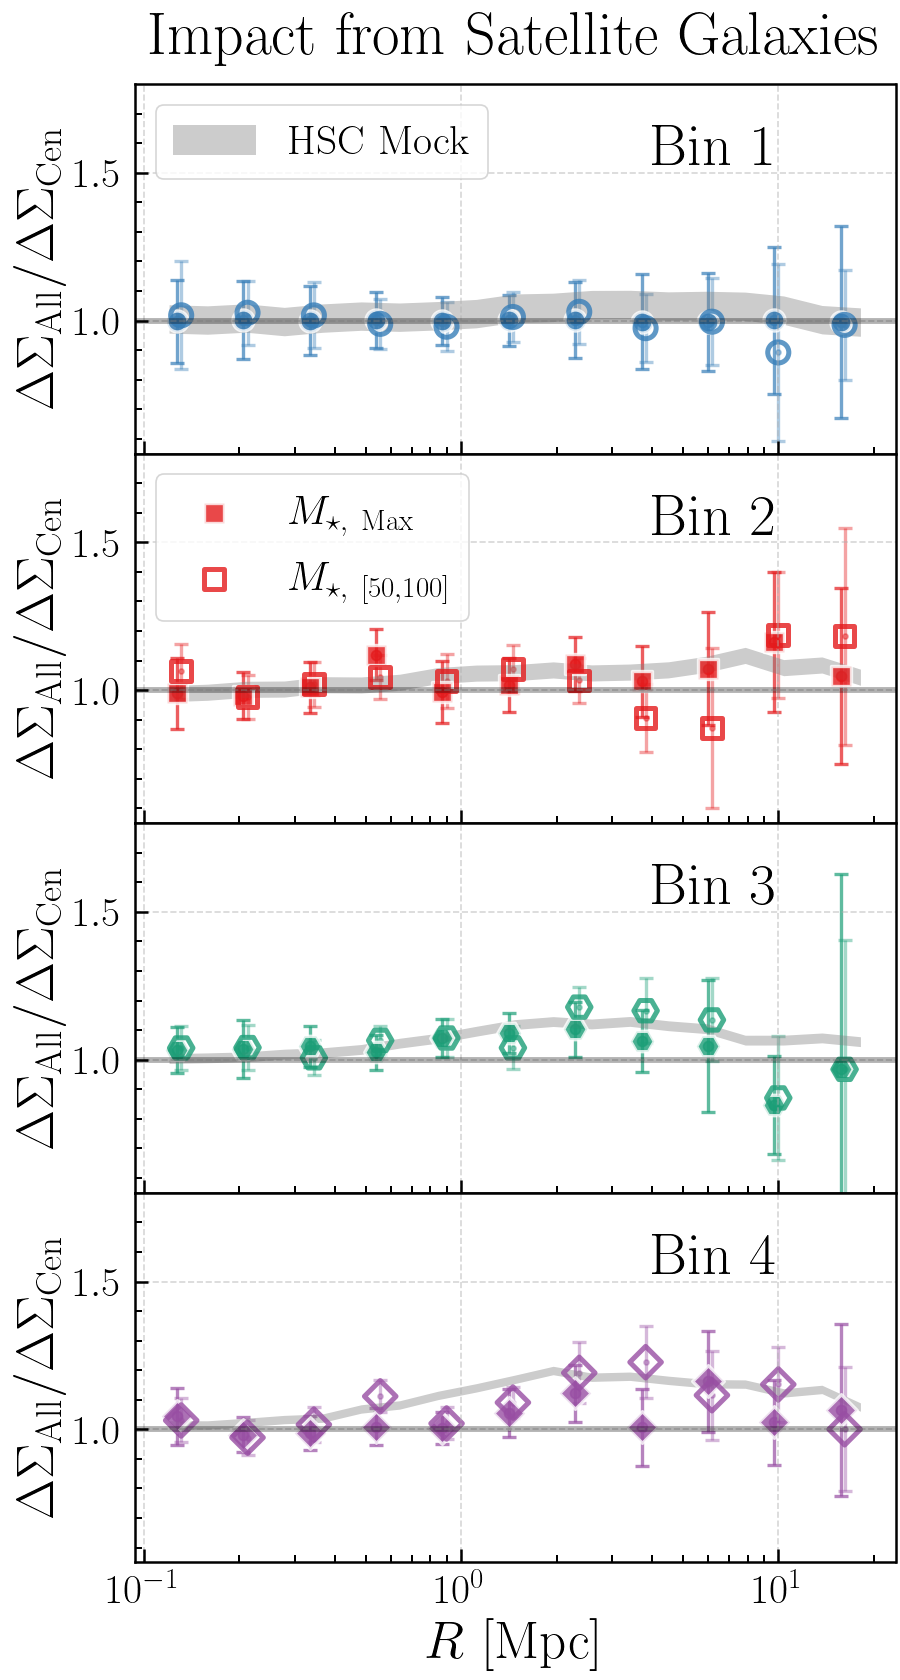
\includegraphics[width=0.47\textwidth]{figure/topn_fig_6}
      \caption{
          Ratio of the \dsigma{} profiles of \topn{} selections of all galaxies (central \&
          satellite; $\Delta\Sigma_{\rm All}$) and only central galaxies ($\Delta\Sigma_{\rm
          Cen}$).
          Grey shaded regions show results from our fiducial HSC mock catalogs.
          Data points show results from HSC data where satellites are removed using a simple
          cylinder based technique.
          We show the ratios of galaxies selected by their \mmax{} (solid symbols) and
          \menve{50}{100} (open symbols; slightly offset along the X--axis).
          Satellites show little impact in the first two bins (corresponding to
          \mmax$> 10^{11.8} M_{\odot}$ and \menve{50}{150}$> 10^{11.1} M_{\odot}$).
          In simulation, including satellites shows a maximum of $\sim 15$\% ($\sim 20$\%) effect
          in Bin 3 (4) at $R\sim 2$--4 Mpc.
          }
      \label{fig:satellite}
  \end{figure}
%% ---------------------------------------------------------------------------------------------- %%

%% ---------------------------------------------------------------------------------------------- %%
%% Impact of satellite galaxies
%% ---------------------------------------------------------------------------------------------- %%
\subsection{Impact of Satellite Contamination on \dsigma{}}
    \label{sec:satellite}

    Although satellite galaxies only make up a small fraction of \logmaper{100}$>$11.5 galaxies
    (e.g., \citealt{More2015, vanUitert2016, Huang2020}), their inclusion could affect our evaluation
    of the performance of \mstar{}-based \mvir{} proxies.
    % Chris added the point about higher bias. Remove if wrong
    Satellites tend to live in less massive halos, but higher bias regions, than centrals
    with the same \mstar{}
    (e.g., \citealt{vanUitert2016, Niemiec2017, Niemiec2019, Dvornik2020, Engler2021}).
    As a result, the \dsigma{} profiles of satellite galaxies show unique "bump"-like features at around
    $R \sim 1$ Mpc (e.g., \citealt{LiShan2014, LiShan2016, Sifon2015, Sifon2018}).
    Comparing this contaminated signal with the pure scatter model could result in incorrect
    estimates of \sigmh{} if the effect is large.

    To compare the \dsigma{} of a pure central sample to that of all galaxies we need to
    populate a mock catalog (where central/satellite assignments are known) or make those
    assignments in data. We do both and compare the results.
    
    Using the fiducial mock catalog (Appendix \ref{app:hsc_model}), we compare the
    \dsigma{} profiles of central galaxies with that of all galaxies.
    The satellite fraction values are [5.0\%, 6.9\%, 8.9\%, \& 10.0\%] in the four \topn{} bins,
    consistent with the low satellite fraction expectation.
    To assign centrals and satellites in the HSC sample, we run a simple algorithm.
    We start from the most massive \mmax{} galaxy and assign as satellites all galaxies
    within a cylindrical region with a 1.0 physical Mpc radius in projection and a 20 
    comoving Mpc length in the line-of-sight (LOS) direction.
    Using this simple strategy, the satellite fractions are [2.0\%, 3.5\%, 3.1\%, \& 8.2\%] 
    in the four bins.
    Since the HSC volume here is much smaller than the \mdpl2{} simulation, and we also use 
    a rather over-simplified method, we do not think the lower satellite fraction values
    from observation is a critical issue for the comparison.

    Figure \ref{fig:satellite} shows the ratio of the \dsigma{} profiles using all galaxies
    and central galaxies in both the mock catalog and HSC data.
    To rank the clusters in HSC we use the maximum 1-D mass \mmax{} and outer envelope mass
    \menve{50}{100} as example proxies.
    In Bin 1 \& 2, We see no impact from satellites in both the mock catalog and HSC data,
    consistent with the low satellite fraction.
    In Bin 3 \& 4, massive satellites lead to a small enhancement in the \dsigma{} profile
    at $R > 500$ kpc compared to the central-only sample.
    In Bin 3 (4), the mock catalog predicts a maximum 10\% (20\%) enhancement at $R \sim 2$-3 Mpc.
    Both \mstar{}-based proxies demonstrate behaviors that are statistically consistent with
    the mock catalog despite the naive satellite-removal method.

    For the remainder of this work, we include massive satellite galaxies in the HSC samples
    and the mock catalogs for the \topn{} tests as it faithfully represents the \mstar{}-based 
    \mvir{} proxy before we can accurately remove satellites.
    The low satellite fractions and their modest impacts on the \dsigma{} profiles ensure that
    this choice will not affects any conclusions. 
    Even for Bin 4 with the largest impact from satellites, a $\sim 10-20$\% enhancement of 
    \dsigma{} profile at $R \sim 2$ Mpc will not affect the comparisons in \S \ref{sec:topn_results}.
    We will discuss more about the impact of satellites in Appendix \ref{app:sat_cen}.

%% ---------------------------------------------------------------------------------------------- %%
%% Trends with scatter
%% ---------------------------------------------------------------------------------------------- %%
% \subsection{Evaluation of \mvir{} Proxies via ``Top N'' Tests}
\subsection{The Amplitude of the \dsigma{} Profile of \mstar{} and Richness Selected Samples}
    \label{sec:topn_results}

    As discussed in \S \ref{sec:estimate_scatter}, the amplitude of the \dsigma{} profile
    is correlated with the scatter between an observable and \mvir{}.
    We now present the \topn{} results, focusing on the amplitude, for a selection of
    observable proxies introduced in \S \ref{sec:proxies}.
    We first describe in detail three proxies which yield interesting results:
    The \mstar in a large aperture (\S \ref{sec:m_aper}), the \mcmodel{} (\S \ref{sec:m100_cmodel}), and the \mstar{} of the outer envelope
    (\S \ref{sec:m100_outskirt}).
    Finally, in \S \ref{sec:trend}, we compare all \mvir{} proxies and present the inferred
    \sigmh{} values given the amplitude of the measured \dsigma{} profiles.


\subsubsection{Aperture \mstar: Optimal Cuts and \dsigma{} Properties}
    \label{sec:m_aper}

    We start by exploring the performance of the aperture stellar mass.
    We show the inferred \sigmvir{} for various apertures in the bottom panel of Figure
    \ref{fig:scatter_trend}. We see that, with increasing aperture size, the \sigmvir{} value decreases,
    across all four bins.
    This decrease is particularly obvious in Bins 1 \& 2 (the most massive halos).
    In Bin 1 (2), \sigmvir{} decreases from 0.63 (0.66) dex for \maper{10}, to 0.52 (0.58)
    dex for \maper{30}, to 0.37 (0.51) dex for \maper{100}.
    This suggests that different parts of massive galaxies follow different SHMRs, and
    the inner 10-30 kpc shows a weaker connection with \mvir{} than the outer envelope.
    Further enlarging aperture size to 150 kpc does not result in a significantly lower
    \sigmvir{} in any of the bins (see Table \ref{tab:summary}).
    It is unclear whether whether the lack of improvement with apertures larger than
    100 kpc reflects the intrinsic limitation of large aperture \mstar{} as a \mvir{} proxy
    or the statistical uncertainty of the current imaging data in the low surface brightness regime.
    Finally, with the exception of \maper{10}, the \sigmvir{} values of \mstar{} proxies all
    increase toward the higher number density end.
    This may suggest that the (intrinsic) scatter of SHMR (across the full profile) also
    becomes larger at the lower \mvir{}-end.

    As the best of the aperture \mstar{} proxies, we will use \maper{100} as the benchmark
    against which we will compare other models in the next few sections.
%% ---------------------------------------------------------------------------------------------- %%
%% Figure: Compare M100kpc mass and CModel mass
%% --------------------------------------------------------------------------------------------- %%
  \begin{figure*}
      \centering
      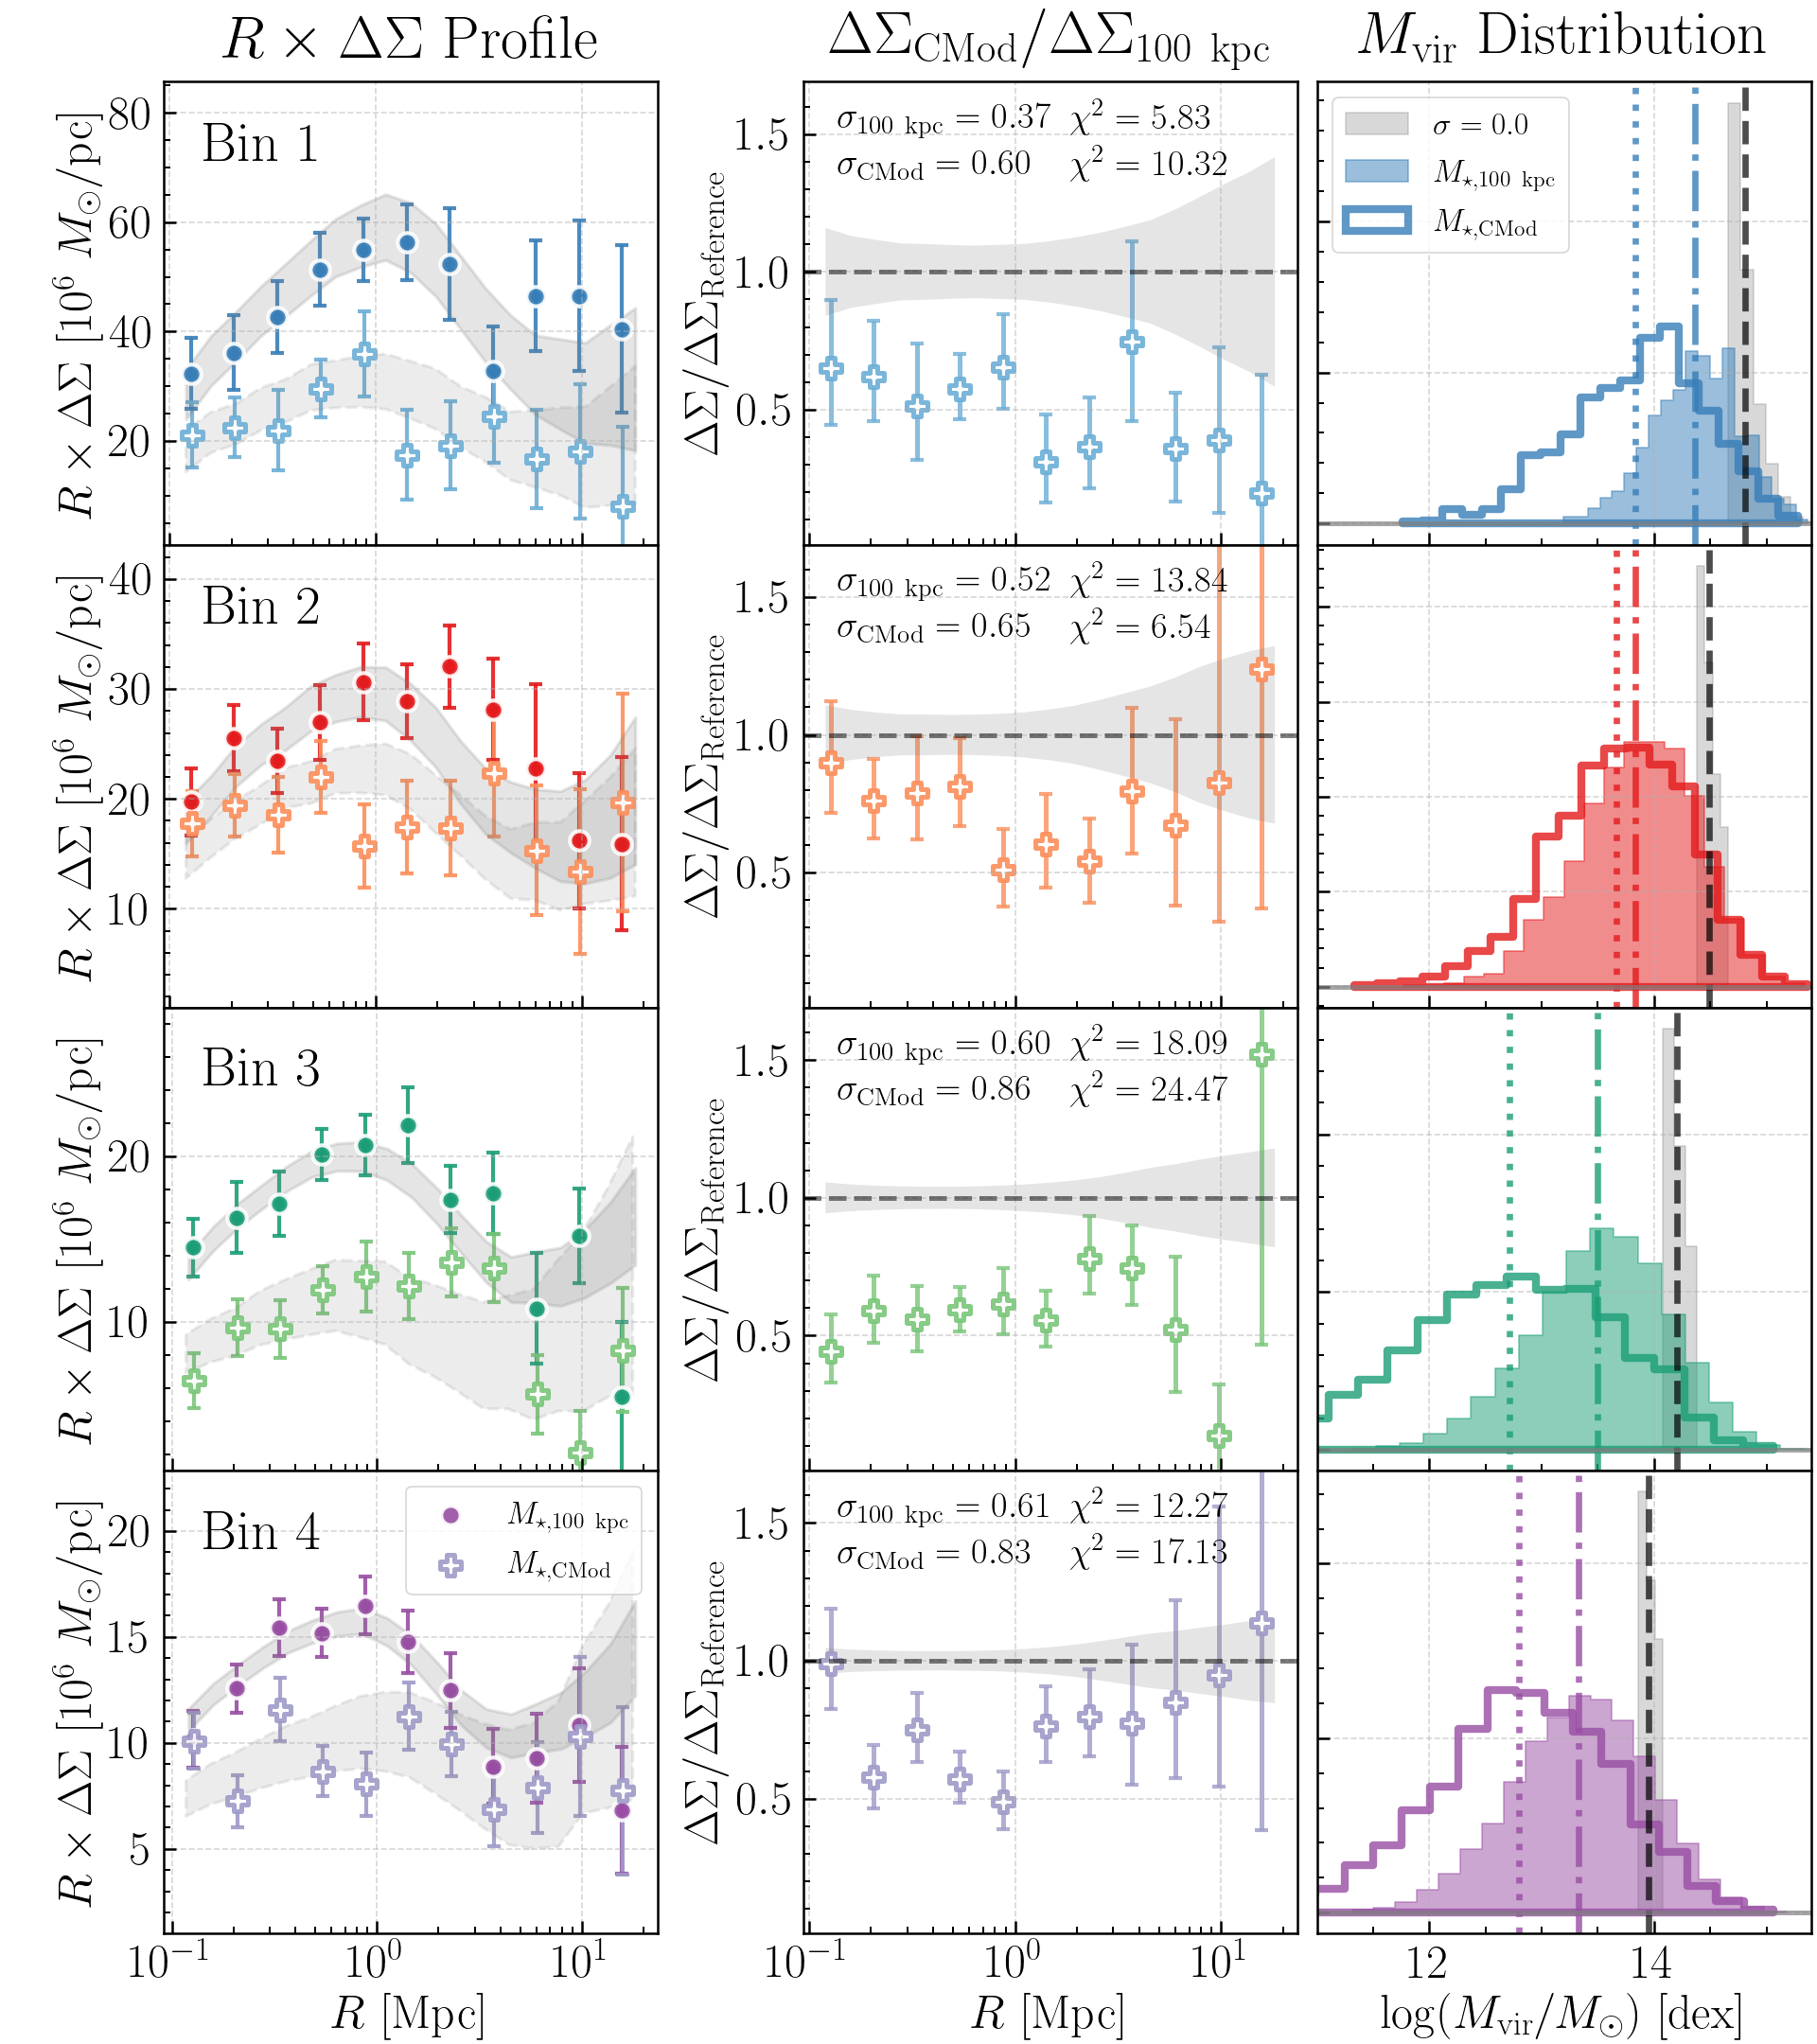
\includegraphics[width=\textwidth]{figure/topn_fig_7}
      \caption{
          The \topn{} test comparison of \maper{100} and \mcmodel{} as \mhalo{} tracers.
          Rows correspond to number density bins (see \S \ref{sec:binning}).
          The \textbf{left} column displays the galaxy-galaxy lensing profiles (\rdsigma{}; circle is
          for \maper{100}; cross is for \mcmodel{}; grey shaded regions show the best-fit
          profiles for \maper{} and \mcmodel{} with typical uncertainties of HSC observations.)
          It is clear that the lensing amplitude for \maper{100} is significantly higher than for
          \mcmodel{} in all four bins.
          Without any model fitting, this figure already demonstrates that \maper{100} is a much
          better tracer of \mhalo{} than \mcmodel{}.
          The \textbf{middle} column shows the ratio of the \dsigma{} profiles of \mcmodel{} and \maper{100}
          selected galaxies.
          The ratio shows weak scale dependence.
          Generally speaking, the \mcmodel{} based selection have lensing amplitudes $\sim$30-50\%
          lower than the \maper{100}--selected samples.
          The \textbf{right} column shows the inferred \mhalo{} distributions for the two samples using the
          model described in \S \ref{sec:estimate_scatter}.
          Grey shaded regions indicate the \mhalo{} distributions of an ideal tracer with
          \sigmh{}$=0$.
          The differences in the mean \mhalo{} between \mcmodel{} and \maper{} based selections
          range from 0.2-0.4 dex in Bin 1 \& 2 and 0.6-0.8 dex in Bin 3 \& 4.
          }
      \label{fig:m100_cmod}
  \end{figure*}
%% ---------------------------------------------------------------------------------------------- %%

%% ---------------------------------------------------------------------------------------------- %%
%% Poor performance of CModel stellar mass
%% ---------------------------------------------------------------------------------------------- %%
\subsubsection{A Large \sigmvir{} for the Default \mcmodel{}}
    \label{sec:m100_cmodel}

    Figure \ref{fig:m100_cmod} shows the performance of \cmodel{} as a \mvir{} proxy by
    comparing its \topn{} results with those of our benchmark aperture stellar mass \maper{100}.
    The \dsigma{} profiles of \mcmodel{}-samples have a significantly lower amplitudes (on average
    by 20-50\%) in all four bins compared to the \maper{100}-samples over the entire radial range (left
    and middle panels of figure \ref{fig:m100_cmod}).
    These results show immediately that the \mcmodel{} selection is significantly worse than the
    \maper{100} one, and thus \mcmodel{} is a worse \mvir{} proxy.

    We want to estimate the scatter in \logmvir{} at a fixed value for each observable by
    matching the observed \dsigma{} profiles to the ``scatter-only'' model profiles as
    described in \S \ref{sec:estimate_scatter}.
    However, we should first check whether the \dsigma{} profiles are consistent with the
    assumptions of this model.
    We can see the \dsigma{} profiles of the \maper{100} samples are statistically
    consistent with the model across all four bins\footnote{In the figure, we inflate the error bars of the
    model profiles to reflect the volume difference between the HSC data and the simulation
    used. For \mdpl2{} simulation, the volume is about $\sim 25 \times$ larger than the HSC
    volume. We therefore increase the error bar by a factor of 5. However, we did not
    include the model uncertainty during the fitting process.} with \chisq{} values of
    $[5.83, 13.84, 18.09, 12.27]$\footnote{Each \dsigma{} profile has 11 data points and
    the scatter of \logmvir{} is the only ``free parameter'' in our model. Therefore one
    can roughly estimate a reduced \chisq{} value using degree-of-freedom $\nu=10$. However,
    given the small sample size in our \topn{} bins, the simple resampling method used to
    estimate covariance matrix, we do not recommend to take the reduced \chisq{} values
    too literately. Relative comparison is a more meaningful way to use these \chisq{} values.}.
    This is an important point, suggesting that a $\log$-normal \mvir{}-observable relation
    model with \emph{just} a Gaussian scatter can already explain the lensing signals at the
    current \snratio{}.
    The \chisq{} values for the \mcmodel{} samples are $[10.32, 6.53, 24.47, 17.13]$,
    considerably worse than for \maper{100}, consistent with the visually poorer fit seen in
    the left panel of Figure \ref{fig:m100_cmod}.

    The best-fit \sigmvir{} values for the \mcmodel{} samples are $[0.60, 0.65, 0.86, 0.83]$,
    much worse than those of \maper{100} samples, $[0.37, 0.52, 0.60, 0.61]$.
    In \S \ref{sec:topn_intro}, we explained that larger \sigmvir{} value also leads to
    lower mean \mvir{} value of the selected sample.
    As shown in the right panel of figure \ref{fig:m100_cmod}, the mean \mvir{} of the
    \mcmodel{} \topn{} samples are $[0.52, 0.17, 0.79, 0.53]$ dex lower than that of
    the \maper{} samples.
    Such a scatter renders the \mcmodel{} essentially useless as \mvir{} proxy.
    Among all the \mvir{} proxies we tested, it is clear that \mcmodel{} has the worst
    performance.
    We will discuss the implications of this in \S \plan{ADD REF}.

%% ---------------------------------------------------------------------------------------------- %%
%% Figure: Compare 50-100 kpc outer envelope mass and 100 kpc mass
%% ---------------------------------------------------------------------------------------------- %%
  \begin{figure*}
      \centering
      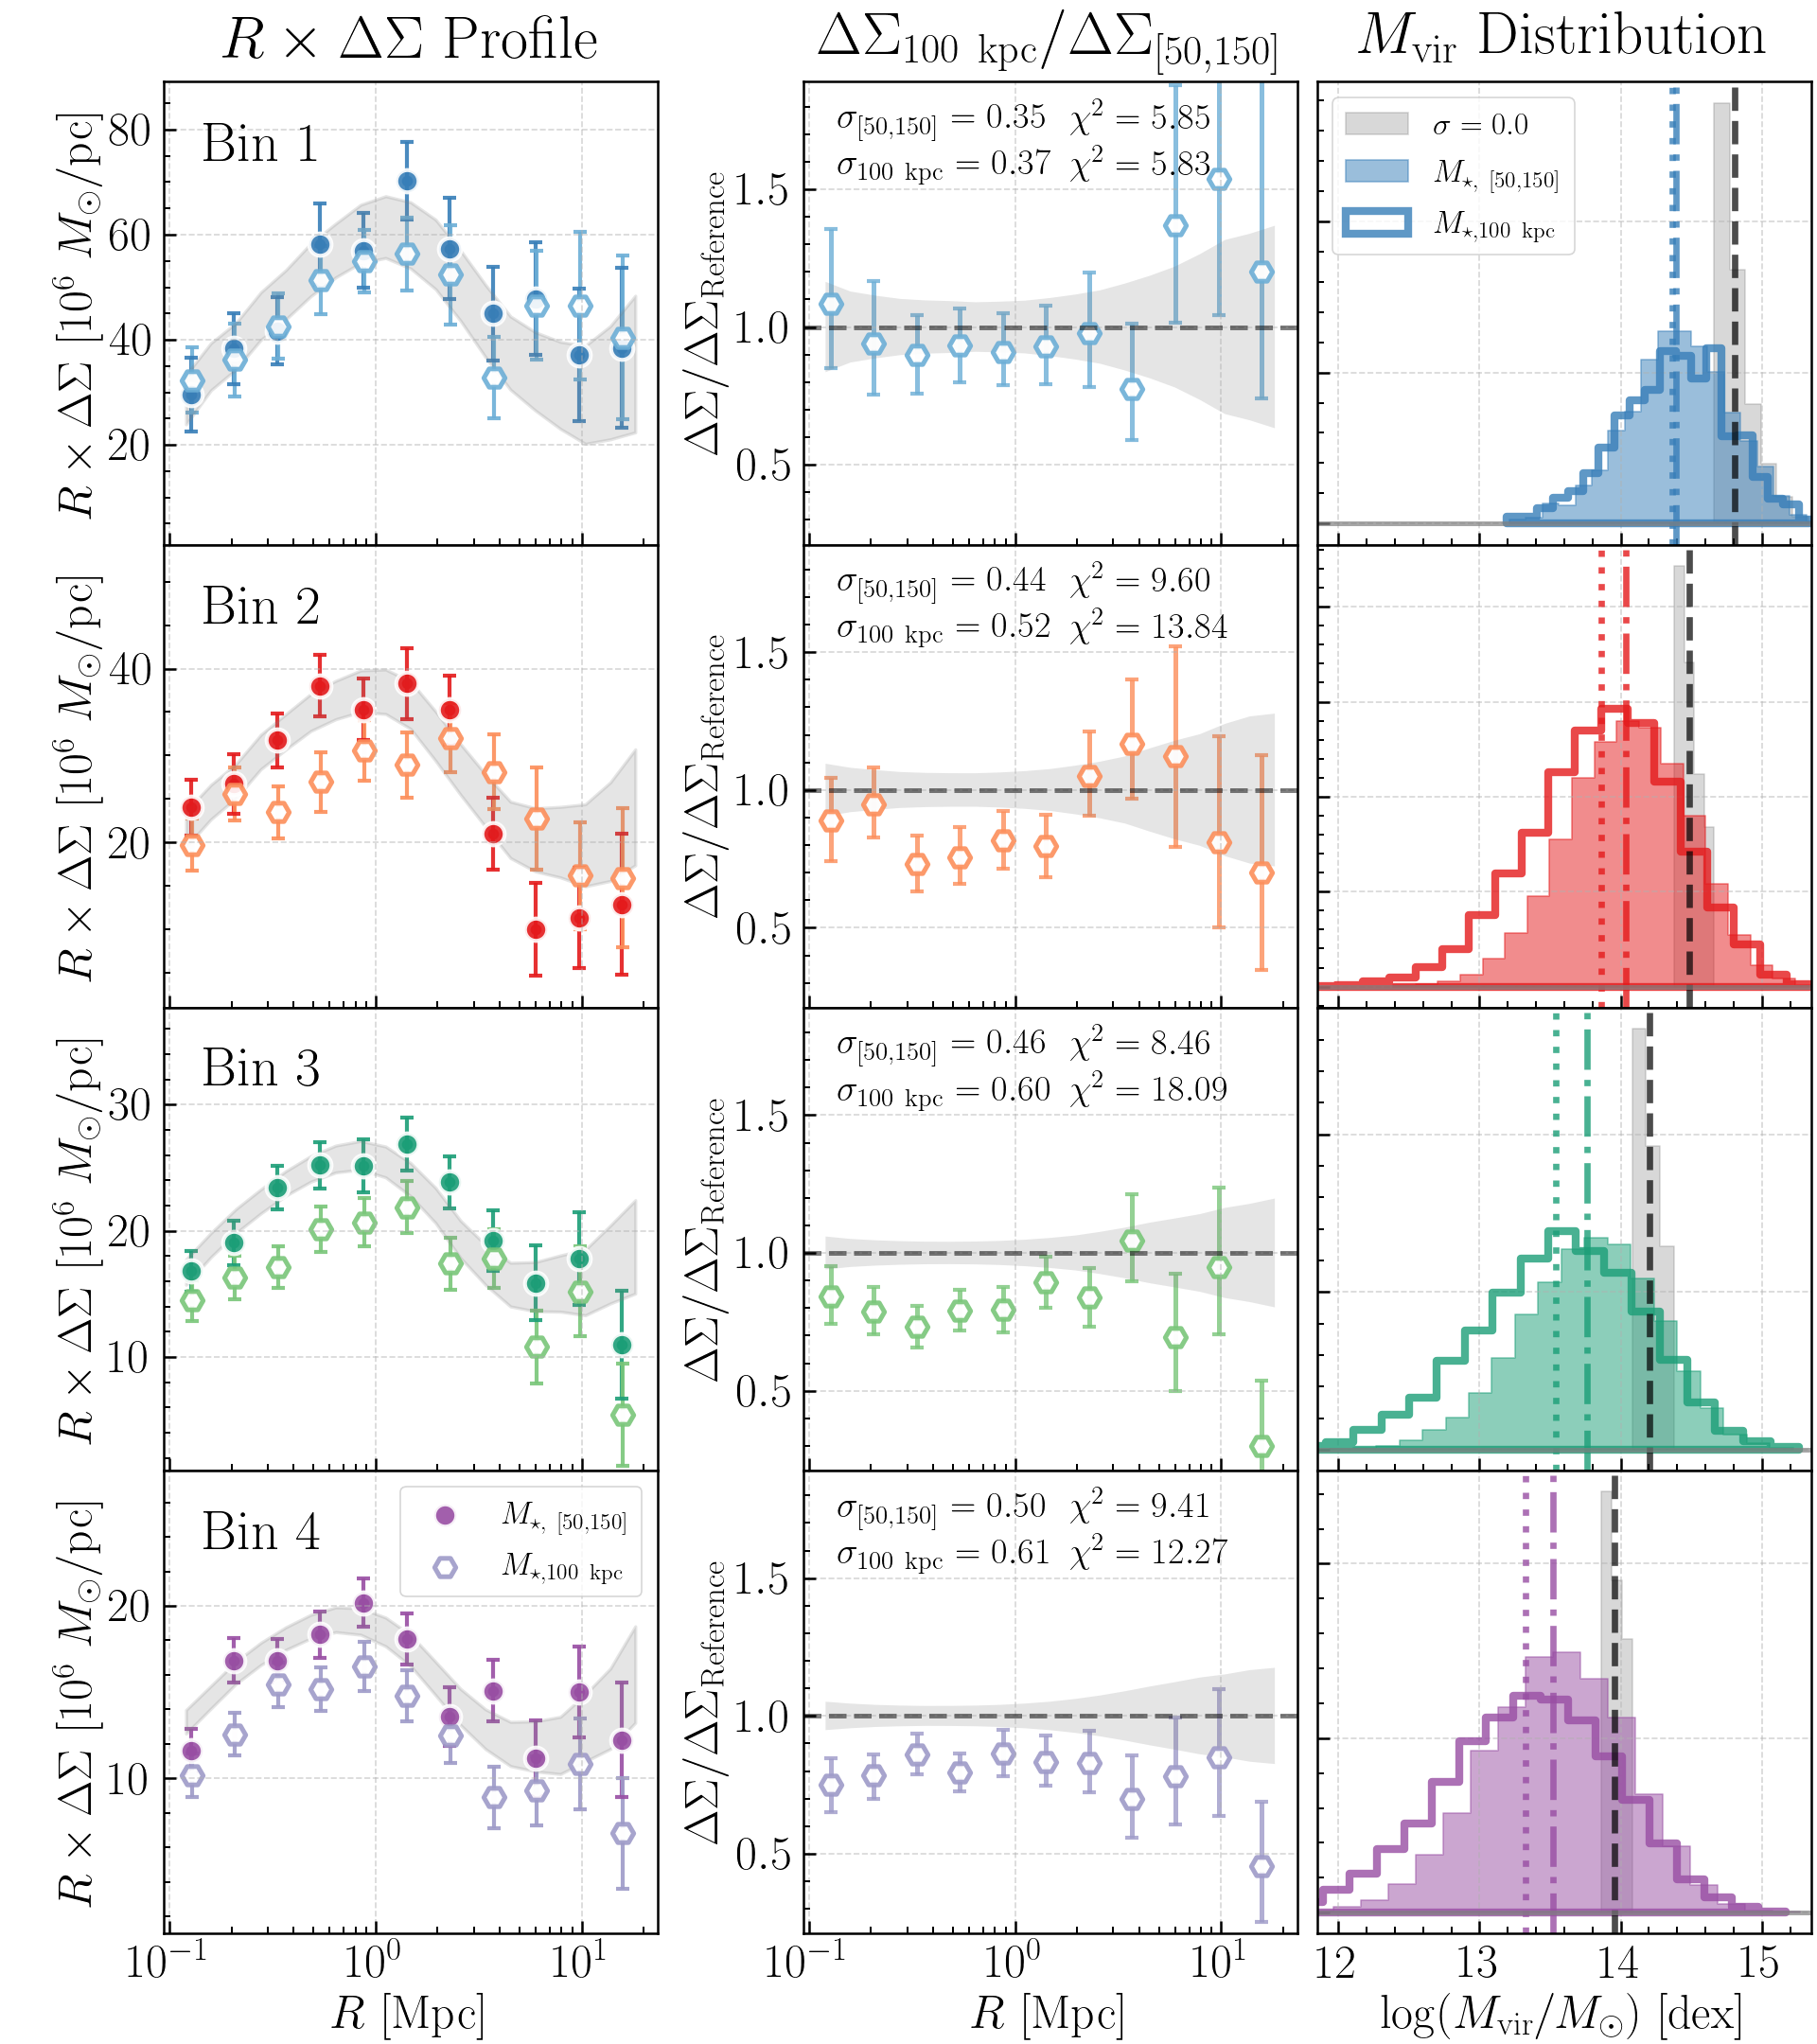
\includegraphics[width=\textwidth]{figure/topn_fig_8}
      \caption{
          The \topn{} comparison of \maper{100} and \menve{50}{150} as \mhalo{} tracers.
          The format of the figure is very similar to Fig \ref{fig:m100_cmod}.
          Solid circle in the left column represents the \rdsigma{} profiles of the \menve{50}{150}
          selected samples while the open-hexagon is for the \maper{100} ones.
          While the lensing profiles are similar in Bin 1, the lensing profile amplitudes of the
          \menve{50}{150} samples are consistently higher in the three other bins than those of
          the \maper{100} samples.
          The \menve{50}{150} selected samples in Bin 2-4 show $\sim 20$--30\% higher \dsigma{}
          amplitude at $R<2$ Mpc regime than the \maper{100} samples (middle column).
          They also show $\sim 0.2$ dex higher average \mvir{} value in the halo mass
          distribution of each bin.
          }
      \label{fig:m100_mout}
  \end{figure*}
%% ---------------------------------------------------------------------------------------------- %%

%% ---------------------------------------------------------------------------------------------- %%
%% Performance of outer envelope mass
%% ---------------------------------------------------------------------------------------------- %%
\subsubsection{Envelope \mstar{}: Optimal Cuts and \dsigma{} Properties}
    \label{sec:m100_outskirt}

    Although much better than the \mcmodel{}, the \maper{100} is still not a great
    \mvir{} proxy and is not on par with richness-based proxies and we have reason to believe
    (as explained in \S \ref{sec:menvelope}) that removing the inner portion of the galaxy and
    using only the outskirts will result in an even better \mvir{} tracer;
    the outskirts likely better represent the \exsitu{} component and the formation scenario
    of massive galaxies suggests that the \exsitu{} stars have a tighter relation with \mvir{}.

    There are no strong predictions from theory about what definition of the envelope best traces
    \mvir{} and so we first compare the inferred scatter from the \dsigma{} profiles of a variety of
    envelope definitions (bottom panel of \ref{fig:scatter_trend_3}).
    This shows that \menve{50}{150} is preferred, possibly optimizing the trade off between retaining
    enough light for a high \snratio{} measurement with removing all \insitu{} stars.
    For example, the performance of \menve{10}{100} is slightly worse than other physical
    envelopes in Bins 2, 3, \& 4, which indicates that we need to look beyond the inner 10-20 kpc
    to remove the noisier inner component.
    We also explore outer envelope definitions using $R_{50}$, but fail to find one whose
    performance is as good as \menve{50}{150}. We discuss these alternate definitions in
    Appendix \ref{app:size}.
    Despite performance changing with envelope definition, all outer envelopes perform better
    than the benchmark \maper{100}, and all other aperture stellar masses (see the top panel
    of \ref{fig:scatter_trend_3}). This strongly suggests that the outer stellar halos of
    low-$z$ massive galaxies are a better tracer of their dark matter halos than the inner parts.

    Figure \ref{fig:m100_mout} shows the detailed comparison between \menve{50}{150} and \maper{100},
    which confirms that, in general, \menve{50}{150} performs better than \maper{100}
    as an \mvir{} proxy in our \topn{} tests.
    With the exception of Bin 1, the \dsigma{} profiles of the \menve{50}{150} samples show
    statistically higher amplitudes at $R < 2$ Mpc than the \maper{100} profiles.
    The difference is more pronounced in lower mass bins as the average
    \dsigma{}$_{100\ \rm kpc}/$\dsigma{}$_{[50,100]}$ ratios are
    $[0.95\pm0.18, 0.85\pm0.13, 0.81\pm0.09, 0.82\pm0.09]$.
    % \chris{I've removed these as this is actually pretty complicated. I can show you plots from the
    % cluster finder where you naturally get these radial dependences even with pure scatter estimators.
    % Basically I'm confident that this is not something interesting about these observables.}
    % The ratios of the \dsigma{} profiles also seem to show radial dependence in Bin 2 \& 3.
    % The differences start to disappear at $R > 2$ Mpc, where the 2-halo terms from
    % nearby environment becomes important.
    As a result, the \sigmvir{} values are also lower for \menve{50}{150}, $=[0.35, 0.44, 0.46, 0.50]$
    compared to $[0.37, 0.52, 0.60, 0.61]$ for \maper{100}.
    Again, the difference is negligible in bin 1, but becomes statistically meaningful in the lower mass bins.
    Finally, the right column of figure \ref{fig:m100_mout} shows the difference in the mass of the selected halos.
    The \menve{50}{150} samples have slightly
    higher mean \mvir{} (\logmvir{}$=[14.39, 14.04, 13.76, 13.52]$) than the
    \maper{100} samples (\logmvir{}$=[14.36, 13.86, 13.54, 13.32]$).
    These conclusions also qualitatively apply to \menve{50}{100}, and do not change
    if we switch \maper{100} with \maper{150}, or \mmax{}.

    Not only does the \dsigma{} profile of the \menve{50}{150} selection fit a lower scatter,
    but the quality of the fit is an improvement over \maper{100} (or \maper{150}, \mmax{}).
    This is particularly true in bins 3 \& 4 where the \chisq{} values are
    $[8.46, 9.41]$ for \menve{50}{150} compared to $[18.09, 12.27]$ for \maper{100}.
    The outer envelope is therefore more consistent with the ``scatter-only'' theoretical model.

    These results robustly demonstrate that \menve{50}{150} (or \menve{50}{100})
    is a better \mvir{} proxy than the large aperture \mstar{} we tested.
    While there theoretical arguments that predict this, there are also practical considerations
    that make it a bit surprising.
    For example, the much more uncertain 1-D profile from the low-\sb{} regime and the
    assumption of constant \mlratio{} should make the outer envelope \mstar{} measurements ``noisier''
    than \maper{100} or \maper{150}.
    The fact that we find better performance with the outer envelope (and assuming that
    the \exsitu{} stars completely dominate these outer envelopes) supports
    the idea that these accreted stellar components have a more intimate
    relation with the underlying dark matter halos.
    It also makes a strong case for the outer envelope \mstar{} as a promising \mvir{} proxy for
    deep imaging.

    The behavior of \menve{10}{100} also almost mirrors the one of \masap{} in the
    top panel (\sigmvir{}$=[0.37\pm0.02, 0.46\pm0.02, 0.52\pm0.02, 0.60\pm0.02]$ dex for
    \menve{10}{100}; $=[0.39\pm0.03, 0.45\pm0.02, 0.51\pm0.02, 0.62\pm0.02]$ dex for \masap{}).
    This shows that the \asap{} model, which uses a linear combination of the \maper{10}
    and \maper{100}, has minimal improvements over one which just uses the difference between
    those masses. This, along with the fact that the preferred envelope mass is between 50 and
    150 kpc, strongly suggests that there is very little information in the inner region of the
    galaxy.
    % We should note that the \dsigma{} profiles of \masap{} samples are well described
    % by the simple ``scatter-only'' model with \chisq{} values of $[8.67, 13.33, 4.95, 9.74]$.

    We recognize that the definition of ``outer envelope'' is not physical in this work, and
    the choice of its inner and outer boundary is somewhat arbitrary.
    We will explore different definitions, including the ones using $R_{50}$ instead of fixed
    physical radius, in \S \ref{sec:trend} and Appendix \S \ref{app:size}.
    And we will also discuss the origin and the implications of this result in
    \S \ref{sec:outskirt_discussion}.

%% ---------------------------------------------------------------------------------------------- %%
%% Figure: Comparisons of scatters: main results
%% ---------------------------------------------------------------------------------------------- %%
  \begin{figure*}
      \centering
      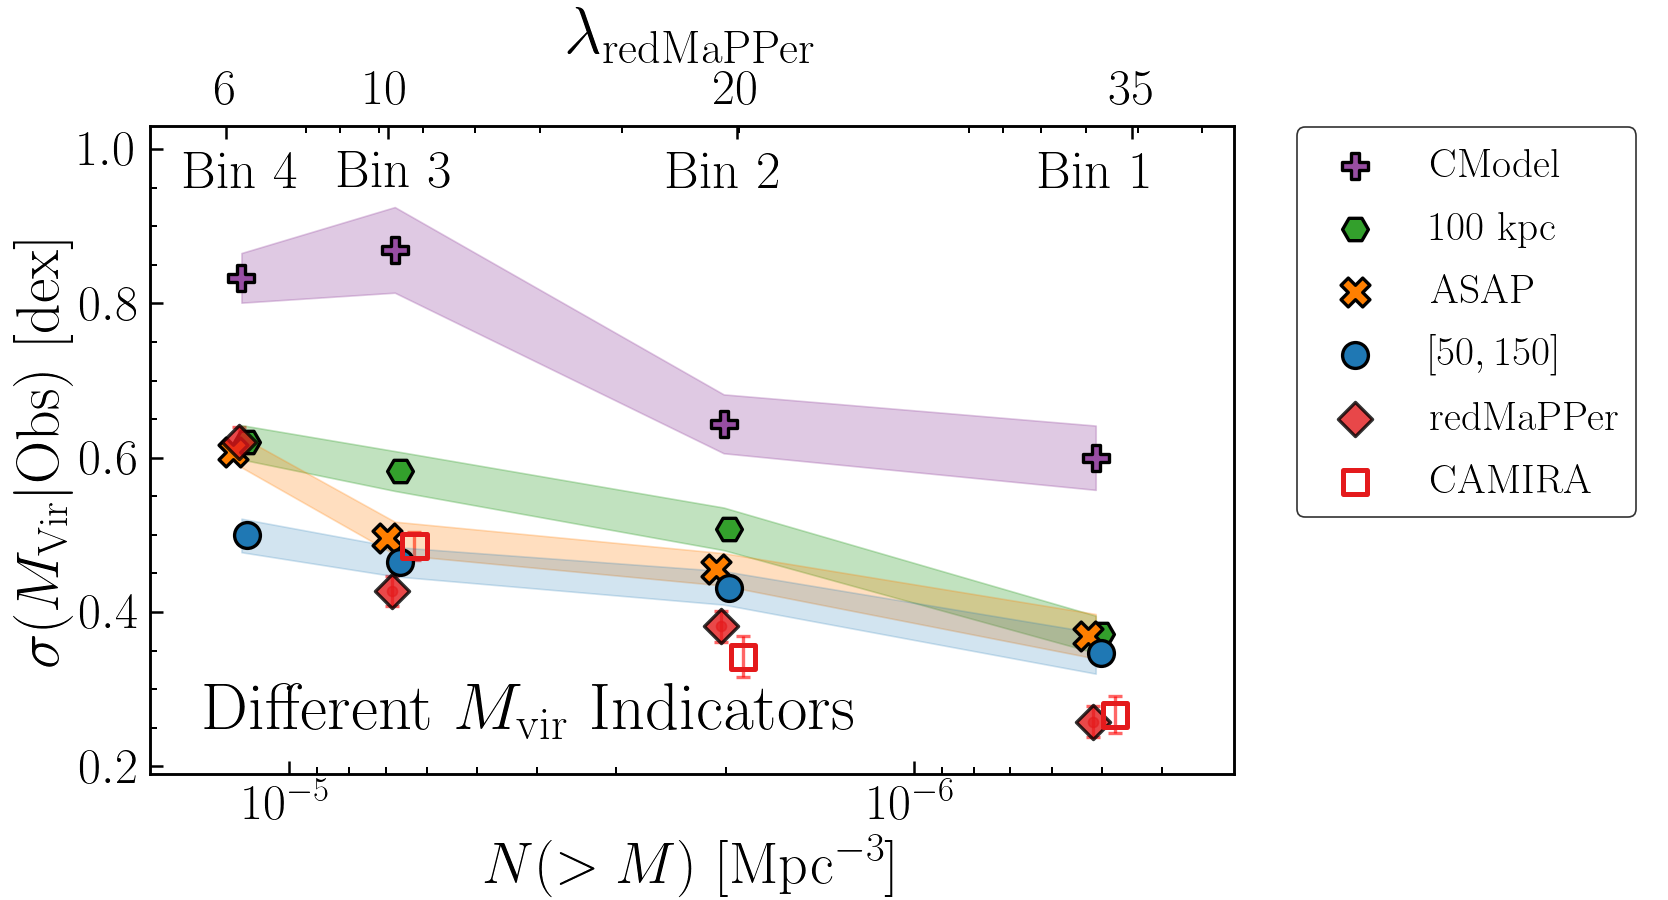
\includegraphics[width=0.85\textwidth]{figure/topn_fig_9a}
      \caption{
          The relations between scatter of \mvir{} and the cumulative number density of each
          \topn{} bin for a few important \mhalo{} proxies. For the X-axis, we show the corresponding
          richness ($\lambda_{\rm redMaPPer}$) threshold of each bin using the HSC \texttt{S16A}
          \redm{} catalog. The Y-axis shows the best-fit scatter of \logmvir{} \emph{for each
          bin} using our simple model. For each \mhalo{} proxy, the shaded region shows the
          uncertainty of the scatter value.
      }
      \label{fig:scatter_trend}
  \end{figure*}
%% ---------------------------------------------------------------------------------------------- %%

%% ---------------------------------------------------------------------------------------------- %%
%% Figure: Comparisons of scatters: different aperture and outer envelope masses
%% ---------------------------------------------------------------------------------------------- %%
  \begin{figure}
      \centering
      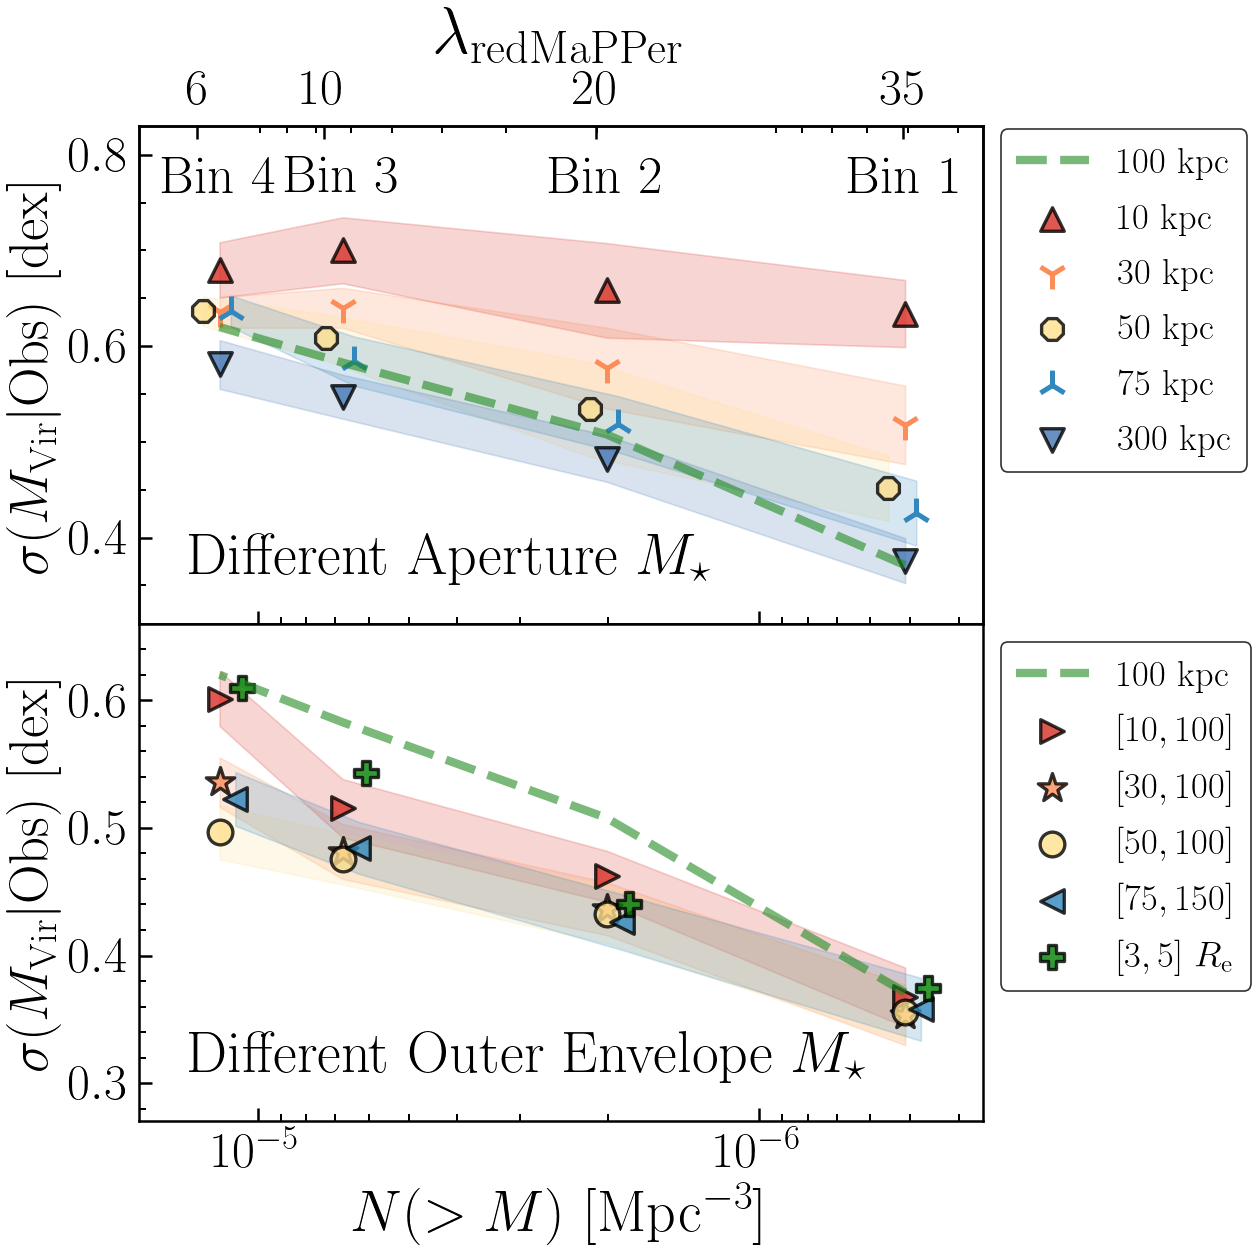
\includegraphics[width=0.49\textwidth]{figure/topn_fig_9b}
      \caption{
          Similar to Figure \ref{fig:scatter_trend}, here we compare the relations 
          between scatter of \mvir{} and the cumulative number density of each
          \topn{} bin for two different groups of \mvir{} proxies. 
          The \textbf{top} panel highlights the trends pf different aperture \mstar{} using the 
          relation of \maper{100} as the reference (green dashed-line). 
          Similarly, we compare different outer envelope \mstar{} in the \textbf{bottom} panel.
          Other formats are the same with Figure \ref{fig:scatter_trend}.
      }
      \label{fig:scatter_trend_3}
  \end{figure}
%% ---------------------------------------------------------------------------------------------- %%

%% ---------------------------------------------------------------------------------------------- %%
%% General trends of scatters
%% ---------------------------------------------------------------------------------------------- %%
\subsubsection{\sigmvir{} of \mstar- and Richness-based Observables}
    \label{sec:trend}

    Having discussed in detail individual observables, and determined the best boundaries for the 
    aperture and envelope \mstar{}, we can now compare the inferred \sigmvir{}
    of the full range of observables (\mstar- and richness-based).
    We emphasize again that for this analysis we \emph{do not exclude} massive satellite galaxies
    from both observations and mock catalogs.
    But, we have shown in \S \ref{sec:satellite} that, due to the low satellite fraction at
    high-\mstar{} end, we see no impact on the \dsigma{} profiles for Bin 1 \& 2 and visible but
    small ($<20$\%) effect at $R>2$-3 Mpc in Bin 3 \& 4.

    Figure \ref{fig:scatter_trend} shows the \sigmvir{} of a set of representative \mvir{} proxies
    using different techniques. These same results, along with the precise cuts that define the
    bin for each proxy can also be found in table \ref{tab:summary}.
    We show the results for \mcmodel{} (default survey photometry), \maper{100} (large aperture
    \mstar{}), \menve{50}{150} (the best outer envelope \mstar{}), \masap{} (a combination of the
    inner and large aperture mass), and $\lambda_{\rm redM,\ HSC}$ and $\lambda_{\rm CAMIRA,\
    HSC}$ (richness of red-sequence galaxies). Note that not all \dsigma{} profiles are well
    described by the ``scatter-only'' model, but we only focus on the best-fit \sigmvir{} values
    here.

    Judged solely by the \sigmvir{} values, the richness of red-sequence galaxies is an
    excellent \mvir{} proxy for cluster-mass halos ($>10^{14} M_{\odot}$).
    All three richness-based cluster finders show lower \sigmvir{} values in Bin 1 \& 2 than
    any of the \mstar{}-based \mvir{} proxies.
    \sigmvir{}$=[0.26, 0.39]$ For HSC \redm{} clusters (Red diamonds in figure
    \ref{fig:scatter_trend}), $[0.26, 0.38]$ dex for the \camira{} \texttt{S16A} catalogs (Red
    squares), and $[0.21, 0.26]$ for the SDSS \redm{} clusters (see Appendix
    \ref{app:sdss_redm}).
    These two bins have \redm{} $\lambda > 20$ and \camira{} $N_{\rm mem} > 21$,
    corresponding to \mvir{}$\geq 1$-$2\times 10^{14} M_{\odot}$.
    In this typical cluster mass regime, such low-\sigmvir{} values computed with our simple
    model qualitatively agree with previous calibrations (e.g., \citealt{Murata2018,
    Murata2019}).

    The \sigmvir{} increases for richness-based proxies towards the lower \mvir{} end.
    For HSC \redm{} clusters, the \sigmvir{} increases to $[0.44, 0.62]$ dex in Bin 3 \& 4,
    while the \sigmvir{} is 0.52 dex in Bin 3 for \camira{} clusters.
    This trend with richness (or number density) is also qualitatively consistent with
    the results from \citet{Murata2018, Murata2019}.
    Taken at face value, the performance of the two richness-based proxies becomes comparable
    with the outer envelope \mstar{} in Bin 3, and is slightly worse in Bin 4.
    However, the $\lambda_{\rm HSC}$ range in Bin 4 ($6 \leq \lambda_{\rm HSC} < 10$) is
    in a low-richness regime that is challenging not only for \redm{}, but any
    richness-based cluster finder.
    But, more importantly, we notice interesting and systematic differences in the \dsigma{}
    profiles of \mstar{}- and richness-samples that make this comparison a pure
    scatter model questionable.
    We discuss this in detail in \S \ref{sec:mstar_vs_richness}.

    Figure \ref{fig:scatter_trend} clearly shows the poor performance of \mcmodel{}
    (\S \ref{sec:m100_cmodel}).
    In all four bins it has \sigmvir{} significantly larger than any of the other
    \mstar- or richness-based proxies.
    However, it also confirms the promising results of \menve{50}{150}, the best of the
    outer envelope proxies (\S \ref{sec:m100_outskirt}). While this has
    scatter not quite comparable to richness in the most massive bins, it is very competitive
    for clusters with $\lambda < 10$.


    To quickly recap the results presented here, the take-home messages from this section are:

    \begin{itemize}

        \item Be careful with the \mstar{} based on default photometry from an imaging survey
            as it is not always optimized to recover the total flux of low-$z$ galaxies. This not
            only applies to \cmodel{}, but could be also true for the small aperture photometry,
            \texttt{SourceExtractor} \texttt{MAG\_AUTO}, or even the single-\ser{} 2-D model.
            Without special attention, they could lead to biased or confusing results.

        \item The outer envelope of massive galaxies is indeed a promising \mstar{}-based
            \mvir{} proxy as it out-performs the total \mstar{} within a large aperture.

        \item Under the ``scatter-only'' model assumption, richness-based \mvir{} proxies
            show impressively low \sigmvir{} values.
            But at the low-richness end (e.g. $\lambda < 10$, or $N_{\rm Mem}<10$),
            \mstar{}-based proxies such as \menve{50}{150} could have an advantage against the
            richness-based ones.

    \end{itemize}


%% ---------------------------------------------------------------------------------------------- %%
%% Figure: Compare 50-100 kpc outer envelope mass and richness selected clusters
%% ---------------------------------------------------------------------------------------------- %%
  \begin{figure*}
      \centering
      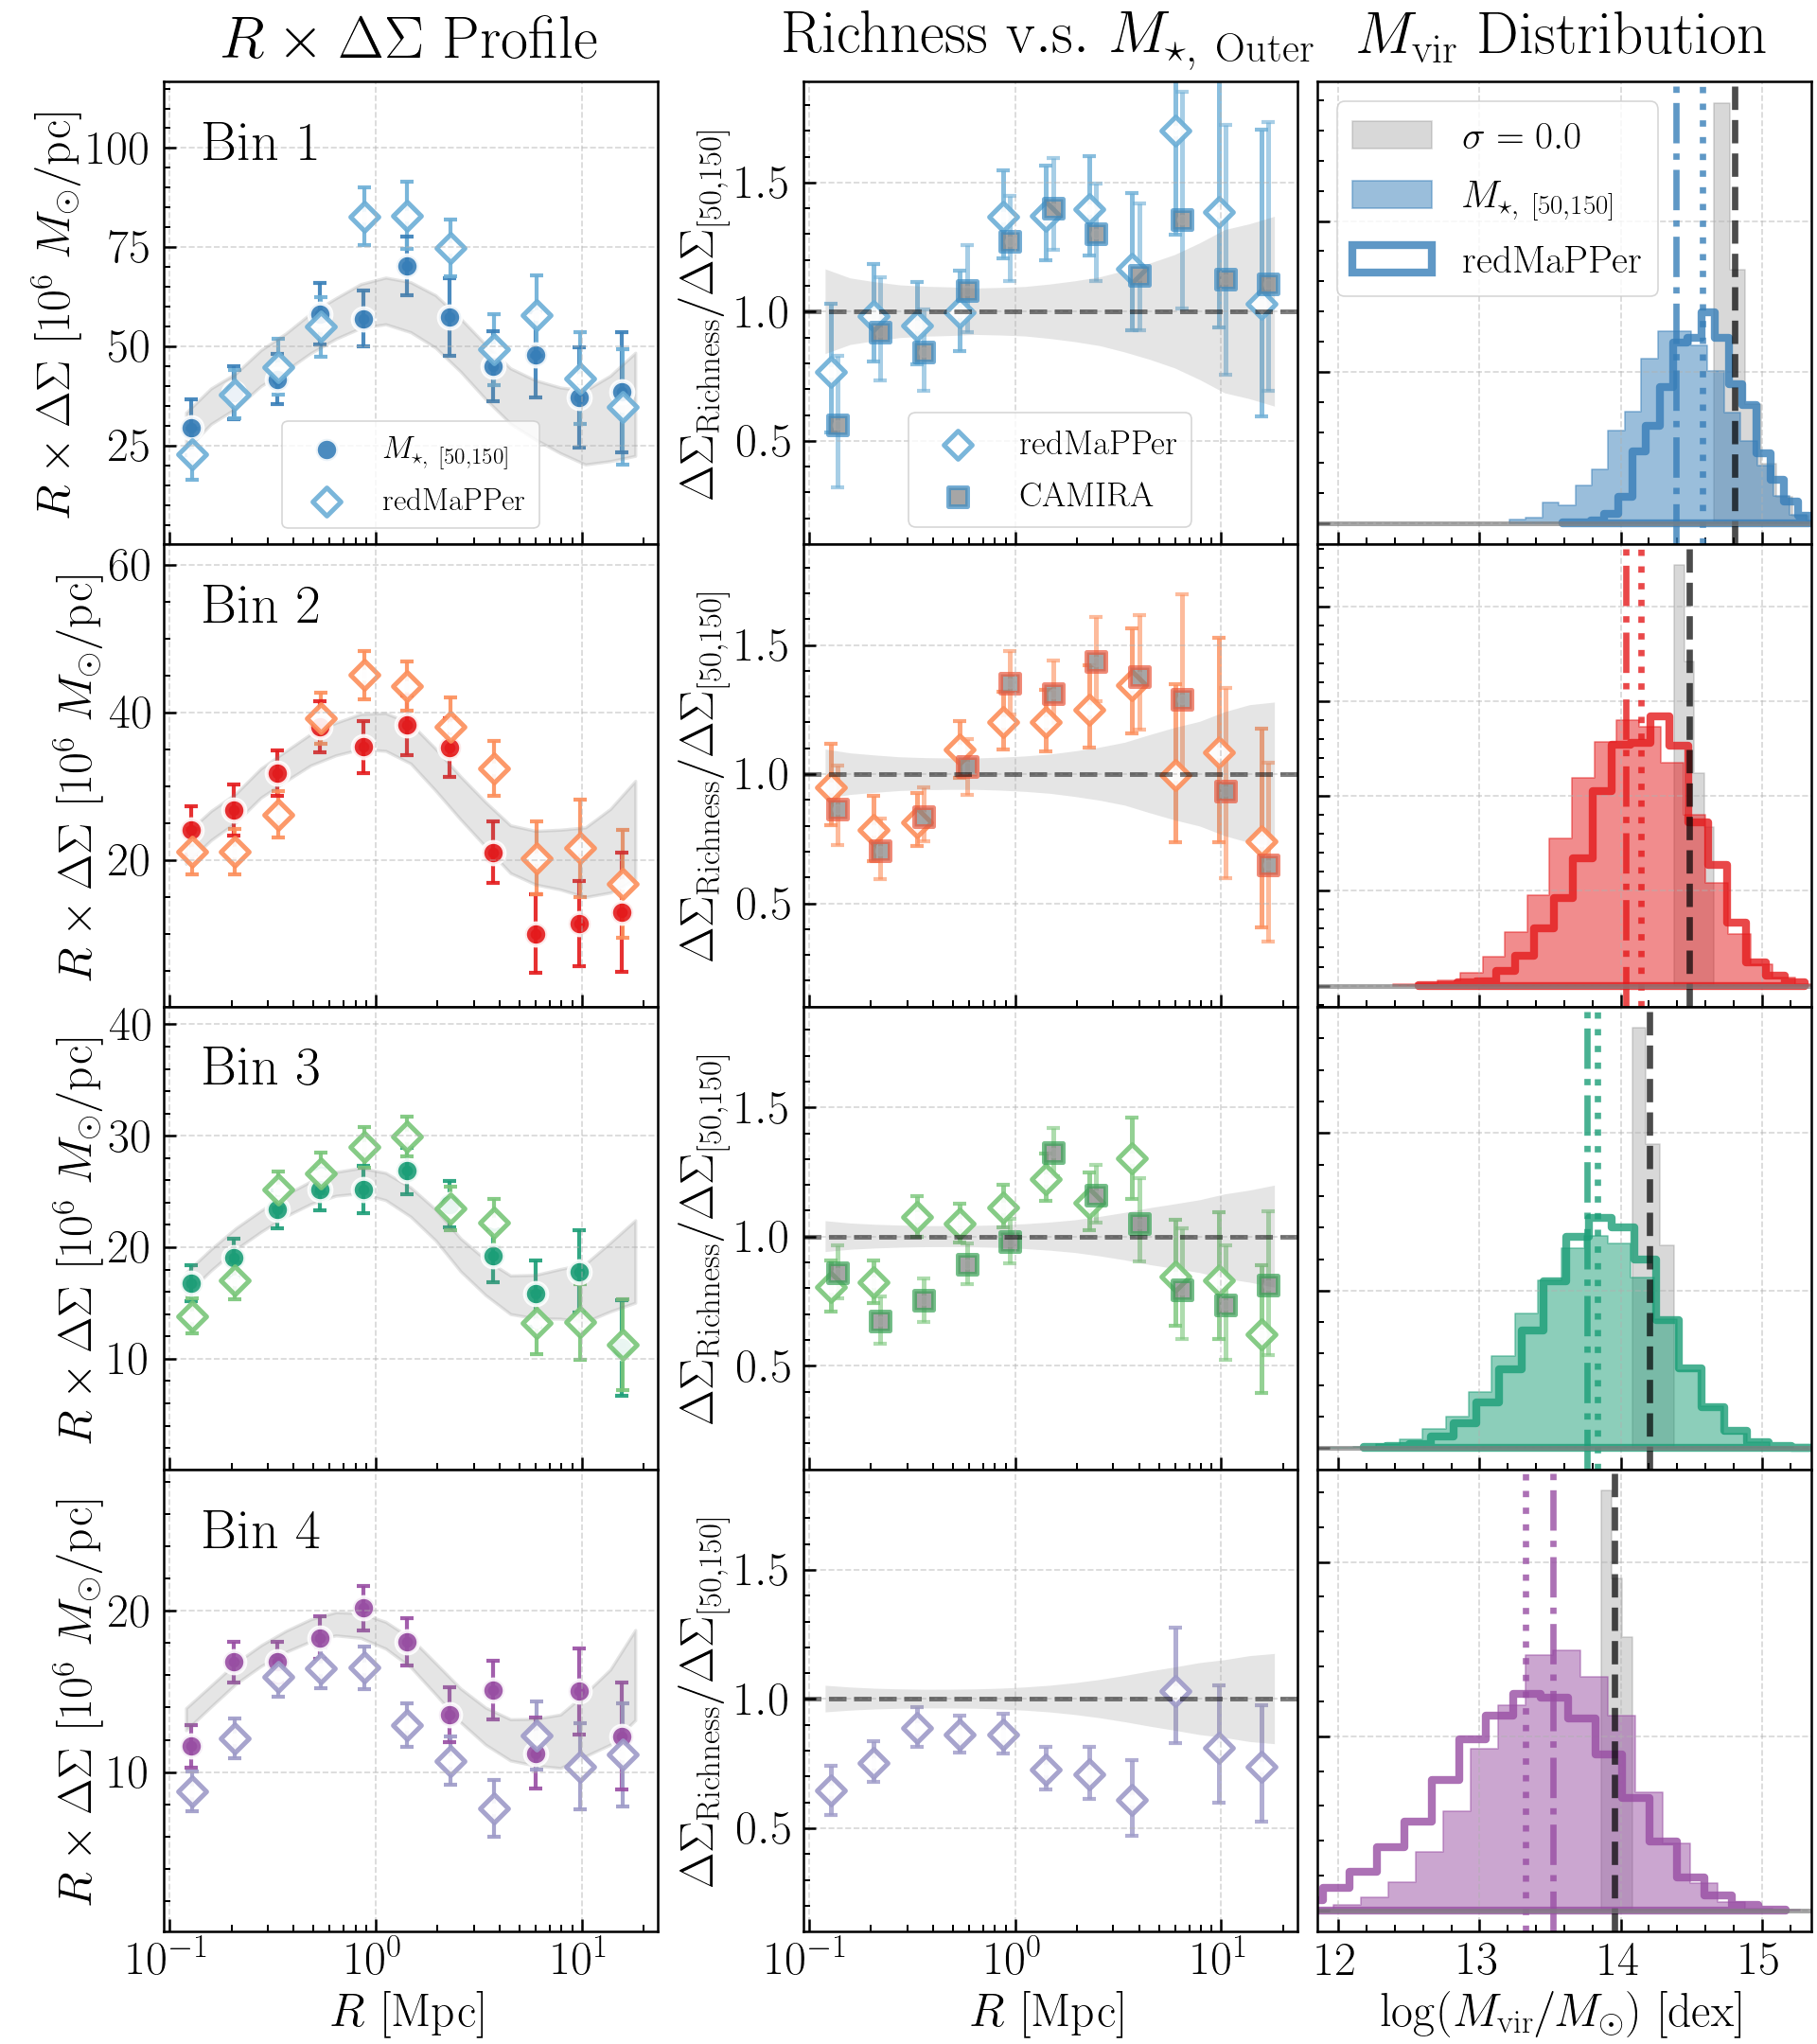
\includegraphics[width=0.95\textwidth]{figure/topn_fig_10}
      \caption{
          \topn{} comparisons between the richness-based optical clusters (\redm{} and \camira{})
          and the massive galaxies selected using outer envelope stellar mass (\menve{50}{150}).
          The layout is very similar to Fig \ref{fig:m100_cmod} and Fig \ref{fig:m100_mout}.
          \textbf{Left} column compares the \rdsigma{} profiles of the HSC \redm{} clusters
          (open diamond) and the \menve{50}{100} (solid circle) selected samples.
          The grey shaded region shows the best-fit profile of the \menve{50}{100} samples.
          In Bin 1-3, while the overall lensing amplitudes are similar, there are interesting
          scale-dependent differences that become more clear using the ratio of the \dsigma{}
          profiles (\textbf{middle} column):
          The lensing amplitudes of \redm{} clusters are systematically higher than the
          \menve{50}{150} samples around $\sim 1$-3 Mpc by $\sim$20--40\%.
          Meanwhile, the amplitudes of \redm{} \dsigma{} profiles are slightly lower than or
          similar to the \menve{50}{150} ones in the central ($R < 0.5$ Mpc) and outer
          ($R>6$-8 Mpc) regions.
          We also show the ratio of lensing profiles using the HSC \camira{} cluster samples
          (square filled with grey color) to highlight the similar behaviour of these two
          richness-based cluster finders.
          In Bin 4, the \redm{} sample displays a $\sim 20-50$\% lower lensing amplitudes than
          the corresponding \menve{50}{150} sample.
          In the \textbf{right} column, we visualize the trend of the average \mvir{} in each bin:
          while the \redm{} samples show $\sim 0.2$ dex higher average \mvir{} value in Bin 1,
          the differences become smaller in Bin 2 \& 3.
          In Bin 4, the \menve{50}{150} selected sample shows a $\sim 0.2$ dex higher average
          \mvir{} values than the \redm{} one instead.
          }
      \label{fig:mout_richness}
  \end{figure*}
%% ---------------------------------------------------------------------------------------------- %%

%% ---------------------------------------------------------------------------------------------- %%
%% Figure: Compare the DSigma profiles of richness selection clusters with their
%%		   best-fit model.
%% ---------------------------------------------------------------------------------------------- %%
  \begin{figure*}
      \centering
      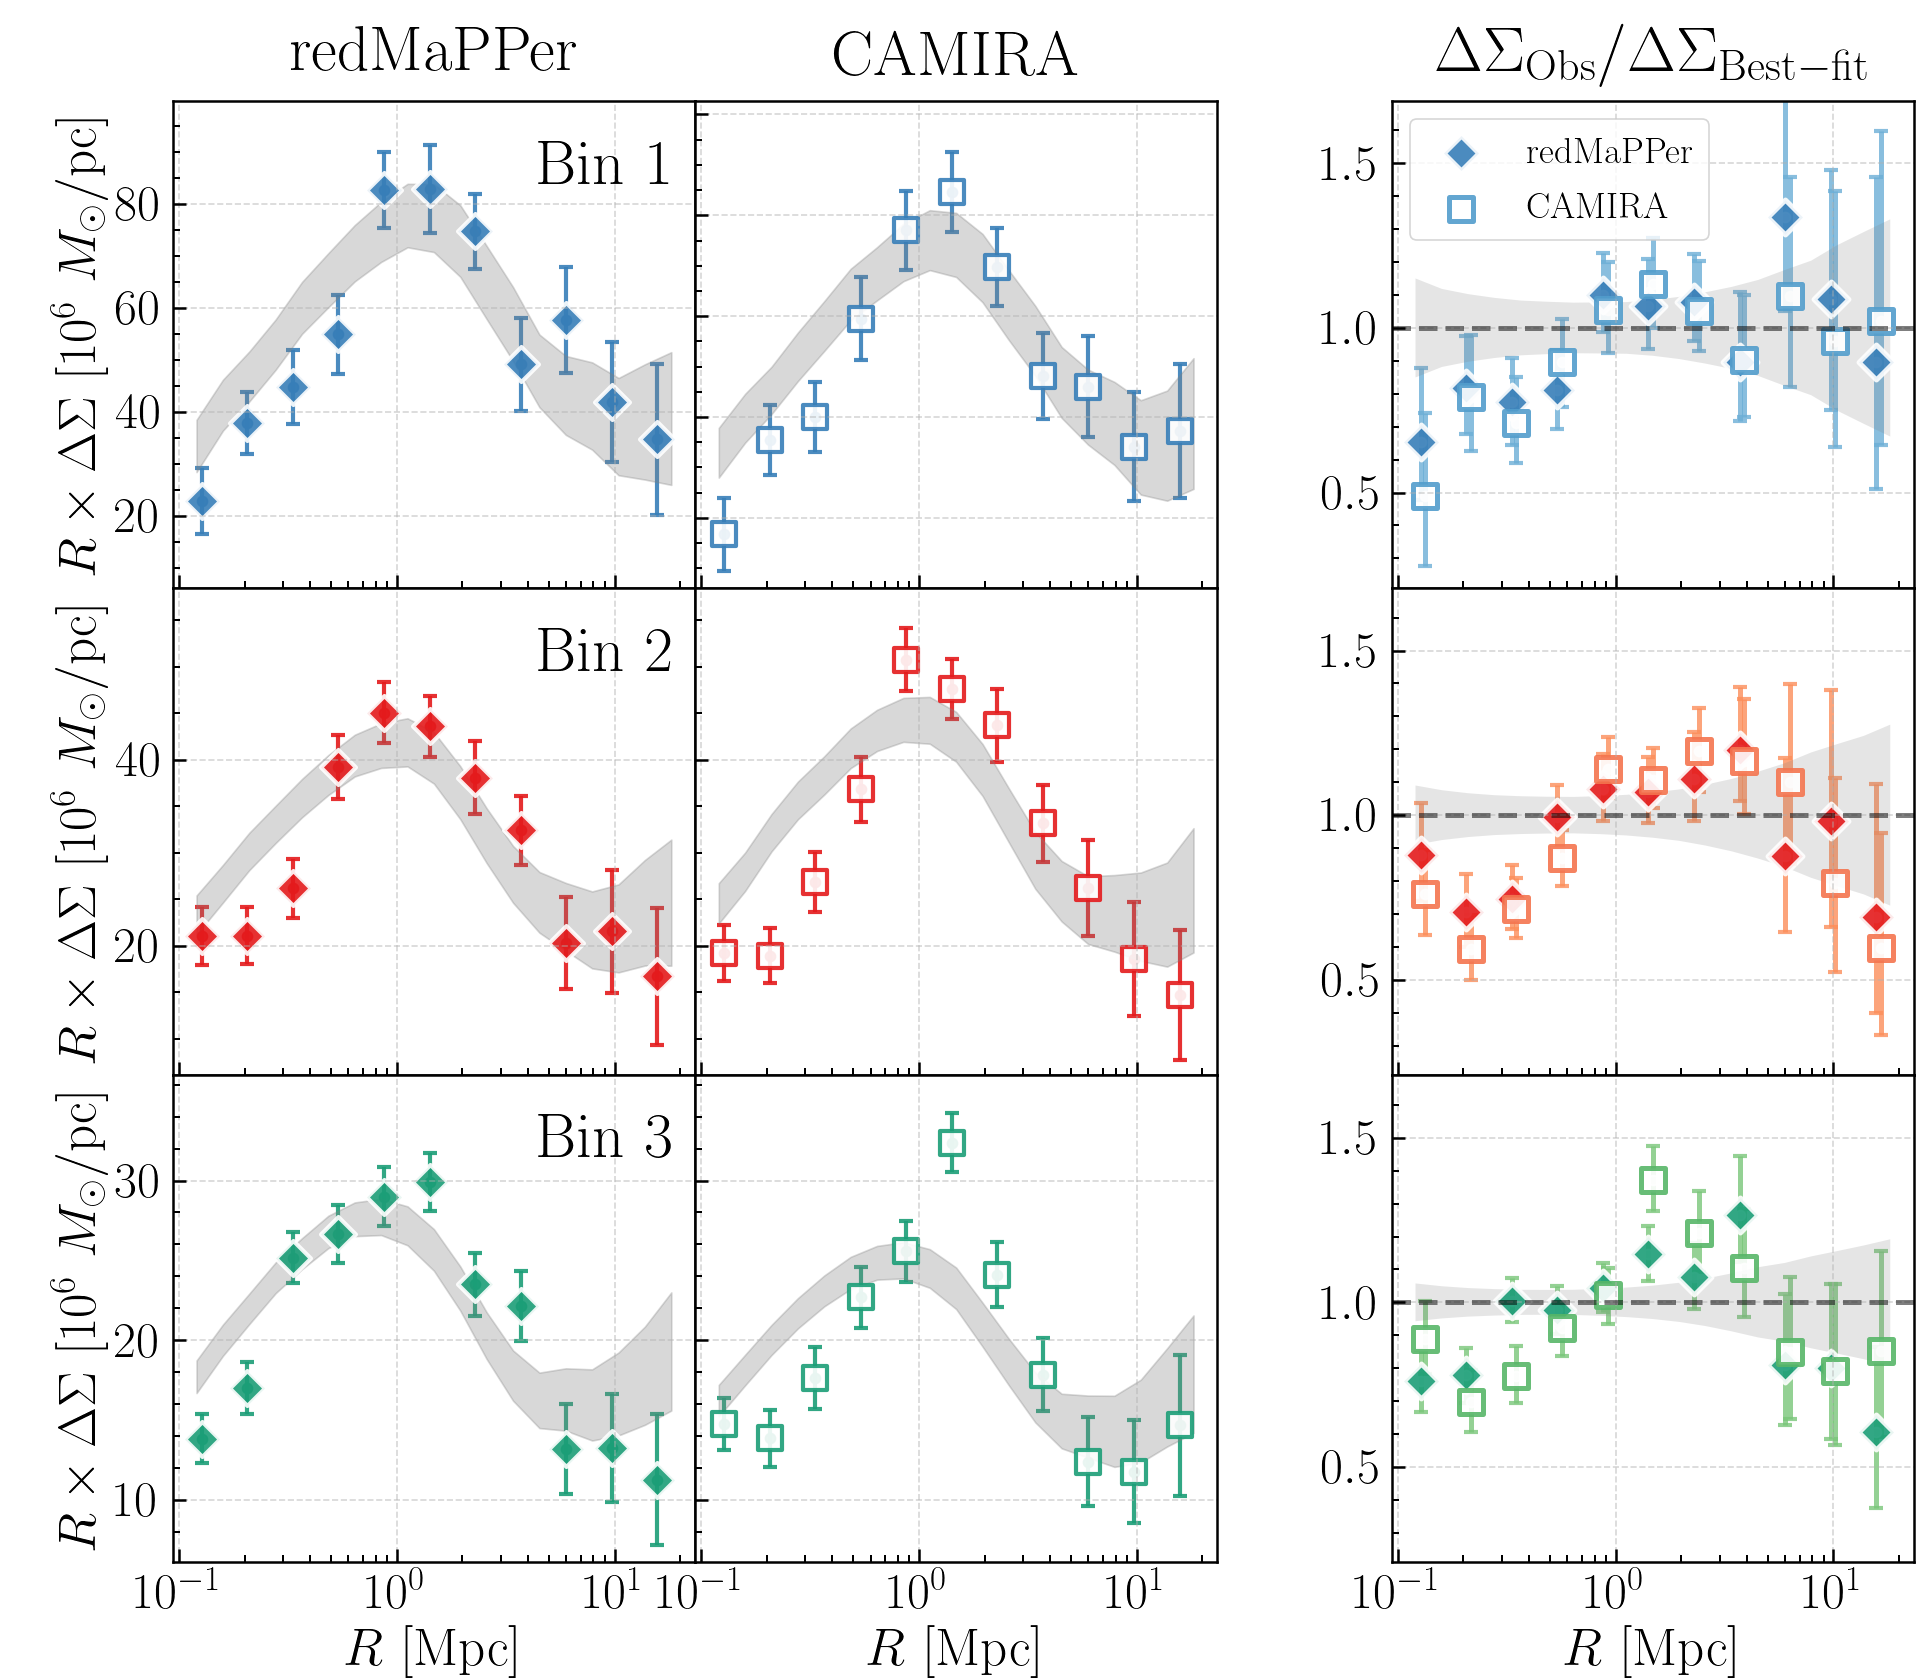
\includegraphics[width=\textwidth]{figure/topn_fig_11}
      \caption{
          Using the HSC \redm{} and \camira{} clusters, we visualize how well our
          ``scatter--only'' model can describe the lensing profiles of richness-selected \topn{}
          samples.
          The \textbf{left and middle} columns show the observed \rdsigma{} profiles (symbols)
          and their best--fit model (grey shaded regions) of the \redm{} (left; filled diamonds)
          and \camira{} (middle; open squares) clusters in Bin 1-3.
          The uncertainties of the model lensing profile are inflated to match the smaller
          HSC volume.
          We ignore Bin 4 since there is not enough \camira{} clusters to fill that number
          density bin and the performance of \redm{} sample there is already worse than some
          \mstar{}-based \mvir{} proxies.
          In the \textbf{right} column, we compare the ratio of the observed \dsigma{} profiles
          to their best-fit model profiles.
          The simple ``scatter--only'' scenario can not model the lensing profiles of these
          clusters and scale-dependent ``residuals'' are clearly visible.
          While the exact values of the ratios are different, the two richness-based cluster
          finders display qualitatively similar behavior: the observed lensing profiles are lower
          than the best-fit models at $R<1$ Mpc by $\sim 30$\% but show higher amplitudes at
          $1-3$ Mpc.
      }
      \label{fig:richness_residual}
  \end{figure*}
%% ---------------------------------------------------------------------------------------------- %%

%% ---------------------------------------------------------------------------------------------- %%
%% Comparison with richness selected galaxies
%% ---------------------------------------------------------------------------------------------- %%
% \subsection{The $\Delta\Sigma$ Profiles of \mstar{} and Richness Selected Samples}
\subsection{The $\Delta\Sigma$ Profile Shape of \mstar{} and Richness Selected Samples}
    \label{sec:mstar_vs_richness}

    While in the previous section we focused on the on the \dsigma{} profile amplitude
    to infer \sigmvir{}, in this section we will look at the profile {\em shape} of the
    richness-selected massive halos with two important questions in mind:

    \begin{enumerate}

        \item Is there any difference between the \dsigma{} profiles of massive halos selected by
            richness and those selected by \mstar{}-based proxies in the same number density bin?

        \item Is the \dsigma{} profile of the richness selected clusters consistent with the
            selection coming from a $\log$-linear \mvir{}-richness relation with Gaussian scatter?

    \end{enumerate}

    As both \redm{} and \camira{} finders have lower \sigmvir{} values in the first two
    \topn{} bins than any \mstar{}-based proxy (\S \ref{sec:trend}, see figure
    \ref{fig:scatter_trend}), we expect their \dsigma{} profiles should also have higher
    amplitudes.
    Similarly, in Bin 3 \& 4, the richness selected \dsigma{} amplitudes should be roughly
    comparable, or slightly below, those of the best \mstar{} proxies such as \menve{50}{150}.

    Figure \ref{fig:mout_richness} compares the \dsigma{} profiles of HSC \redm{}, \camira{} clusters
    (first three bins only), and \menve{50}{150}-selected massive halos.
    The middle column shows the ratio of the richness selected \dsigma{} to the \menve{50}{150}
    to highlight any differences.
    In Bin 1 to 3, both \redm{} and \camira{} \dsigma{} profiles show similar
    systematic differences in shape when compared to the \menve{50}{150}.
    The most prominent difference is that, between $1 < R < 3$ Mpc, the richness-based \dsigma{}
    profiles demonstrate significantly enhanced ($\sim 30$-40\%) \dsigma{} amplitudes.
    On the other hand, at $R < 1$ Mpc, the \dsigma{} profiles of \redm{} and \camira{} samples
    are $\sim 20$-40\% lower than the outer envelope \mstar{} ones.
    At larger scale ($R > 5$ Mpc), we find that the richness-based and \menve{50}{150} \dsigma{}
    profiles become statistically similar but we are also limited by the low \snratio{} of the
    current profiles.
    Replacing \menve{50}{150} with other \mstar{}-based proxies that show similar \sigmvir{}
    values (e.g., \maper{100}, \masap{}, \menve{50}{100}, and many others) does not
    qualitatively change this difference in shape, it merely shifts the ratio of \dsigma{} profiles
    vertically by a little.
    SDSS \redm{} clusters also show similar results in Bin 1 \& 2 (see Appendix
    \ref{app:sdss_redm}).
    Despite the small sample size in each bin, consistent results from different combinations
    of cluster finders and \mstar{}-based proxies confirm the robustness of this systematic
    difference.

    Thus, while we would expect the lower inferred \sigmvir{} to translate primarily into a
    profile shifted up compared to \mstar{}-based proxies, instead we find an entirely different
    profile shape.
    Instead of globally higher amplitudes in the 1-halo term dominated region, the
    richness-based \dsigma{} profiles show a ``bump''-like feature at $R \sim 1$-2 Mpc,
    which is roughly coincident with the transitional region between 1-halo and 2-halo terms.
    It is unclear what causes this feature, but leads to the second question -- could these profiles
    come from halos selected by an observable with a log-linear relationship to \mvir{} and
    Gaussian scatter?

    % In Bin 4, the \redm{} \dsigma{} profile falls below the \menve{50}{150} ones at
    % $R < 5$ Mpc by $\sim 15$-40\%.
    % This is consistent with their \sigmvir{} values (Figure \ref{fig:scatter_trend}) and the
    % inferred \mvir{} distributions shown in the right panel of Figure \ref{fig:mout_richness}.
    % The \menve{50}{150} sample in Bin 4 has mean \logmvir{}$=13.58$, much lower than the
    % typical ``galaxy cluster'' definition.
    % This ``massive group'' regime may become fundamentally challenging for richness-based
    % \mvir{} proxy.

    To address this second question, figure \ref{fig:richness_residual} compares the \dsigma{}
    profiles of \redm{} and \camira{} samples to their best-matched profiles in our
    ``scatter-only'' model (\S \ref{sec:estimate_scatter}) in the first three \topn{} bins.
    It is abundantly clear that these richness-based samples' \dsigma{} profiles cannot be
    well-described by this simple model.
    The \chisq{} values of the ``best-fit'' models are $[18.33, 24.89,
    40.78]$ for the HSC \redm{} clusters and $[18.60, 63.16, 52.51]$ for the \camira{}
    \texttt{S16A} samples, which are much worse than the \menve{50}{150} values of
    $[5.85, 9.60, 8.46]$.

    The right column of Figure \ref{fig:richness_residual} highlights the relative residuals
    of these models.
    The \redm{} and \camira{} profiles show residual patterns that are statistically
    consistent with each other.
    The deviations from the ``best-fit'' models are not only significant but also resemble
    the ratio of \dsigma{} profiles with \menve{50}{150} (middle panels of Figure
    \ref{fig:mout_richness}) which we have already shown is consistent with the best fit model.
    The most prominent feature in the residuals is the strongly suppressed $R < 1$ Mpc
    region (up to $\sim 50$\%) in the observed \dsigma{} profiles of richness-selected
    clusters.
    % The model fitting process seems to put more emphasis in the outer region, and attempts
    % to fit the $R \sim 1$-2 Mpc region as well as it can.
    % For example, in Bin 1, the \dsigma{} profiles at $R > 1$ Mpc are both well-fit by the
    % ``scatter-only'' model.
    The high amplitude around 1 Mpc in the model \dsigma{} profile directly leads to the higher
    \mvir{} distribution and lower \sigmvir{} values we see, but it also makes the systematic 
    deviations in the inner region more significant.
    A similar scenario is seen in Bins 2 \& 3, though here we also see a suppression of \dsigma{}
    at large radii to go with the suppression at small radii and the ``bump'' around $R = 1$Mpc.
    % But the observed \dsigma{} profiles there at at $R > 1$ Mpc can not be perfectly described
    % by the model, hence we can still see the hints of the ``bump'' features, especially
    % for the \camira{} profiles.

    These results reinforce our conclusion: unlike the \mstar{}-based \mvir{} proxies,
    the \dsigma{} profiles of richness-based clusters and their \mvir{} distributions can not
    be modeled by a simple $\log$--normal \mvir{}-richness relation with Gaussian scatter.
    This is in line with previous models of cluster \dsigma{} profiles (e.g.,
    \citealt{Melchior2017, Murata2018, McClintock2019}), but our result clearly illustrates
    this point without assuming the contributions from different ``components'' in the \dsigma{}
    profile.
    We should point out that the systematic difference of \dsigma{} profiles observed here may 
    relates to the selection bias in the richness-selected cluster samples 
    (e.g., \citealt{Sunayama2020, DES2020}).
    We will discuss this more in \S \ref{sec:perfect_finder}.

%% ---------------------------------------------------------------------------------------------- %%
%% Discussion
%% ---------------------------------------------------------------------------------------------- %%
\section{Discussion}
    \label{sec:discussion}
    
    Now we briefly discuss the implications of the results presented in this work. 
    In \S \ref{sec:outskirt_discussion}, we will focus on outer envelope \mstar{}'s potential 
    as a great \mstar{}-based \mvir{} proxy.
    \S \ref{sec:perfect_finder} summarizes our thoughts on how to search for better \mvir{} proxy
    and improve cluster finder in the near future.

    Before we dive in, we want to remind the readers that
    1) All the \sigmh{} values mentioned in this work are the scatter of \mvir{} \emph{within each
    number density bin}. 
    We do not attempt to calibrate or forward-model the \mvir{}-observable
    relation, therefore we can not predict the scatter of \mvir{} \emph{at any given value of
    the observable}.
    2) All the \sigmh{} values should be treated in a relative sense.
    
%% ---------------------------------------------------------------------------------------------- %%
%% Figure: Discussion about the outskirt stellar mass
%% ---------------------------------------------------------------------------------------------- %%
  \begin{figure*}
      \centering
      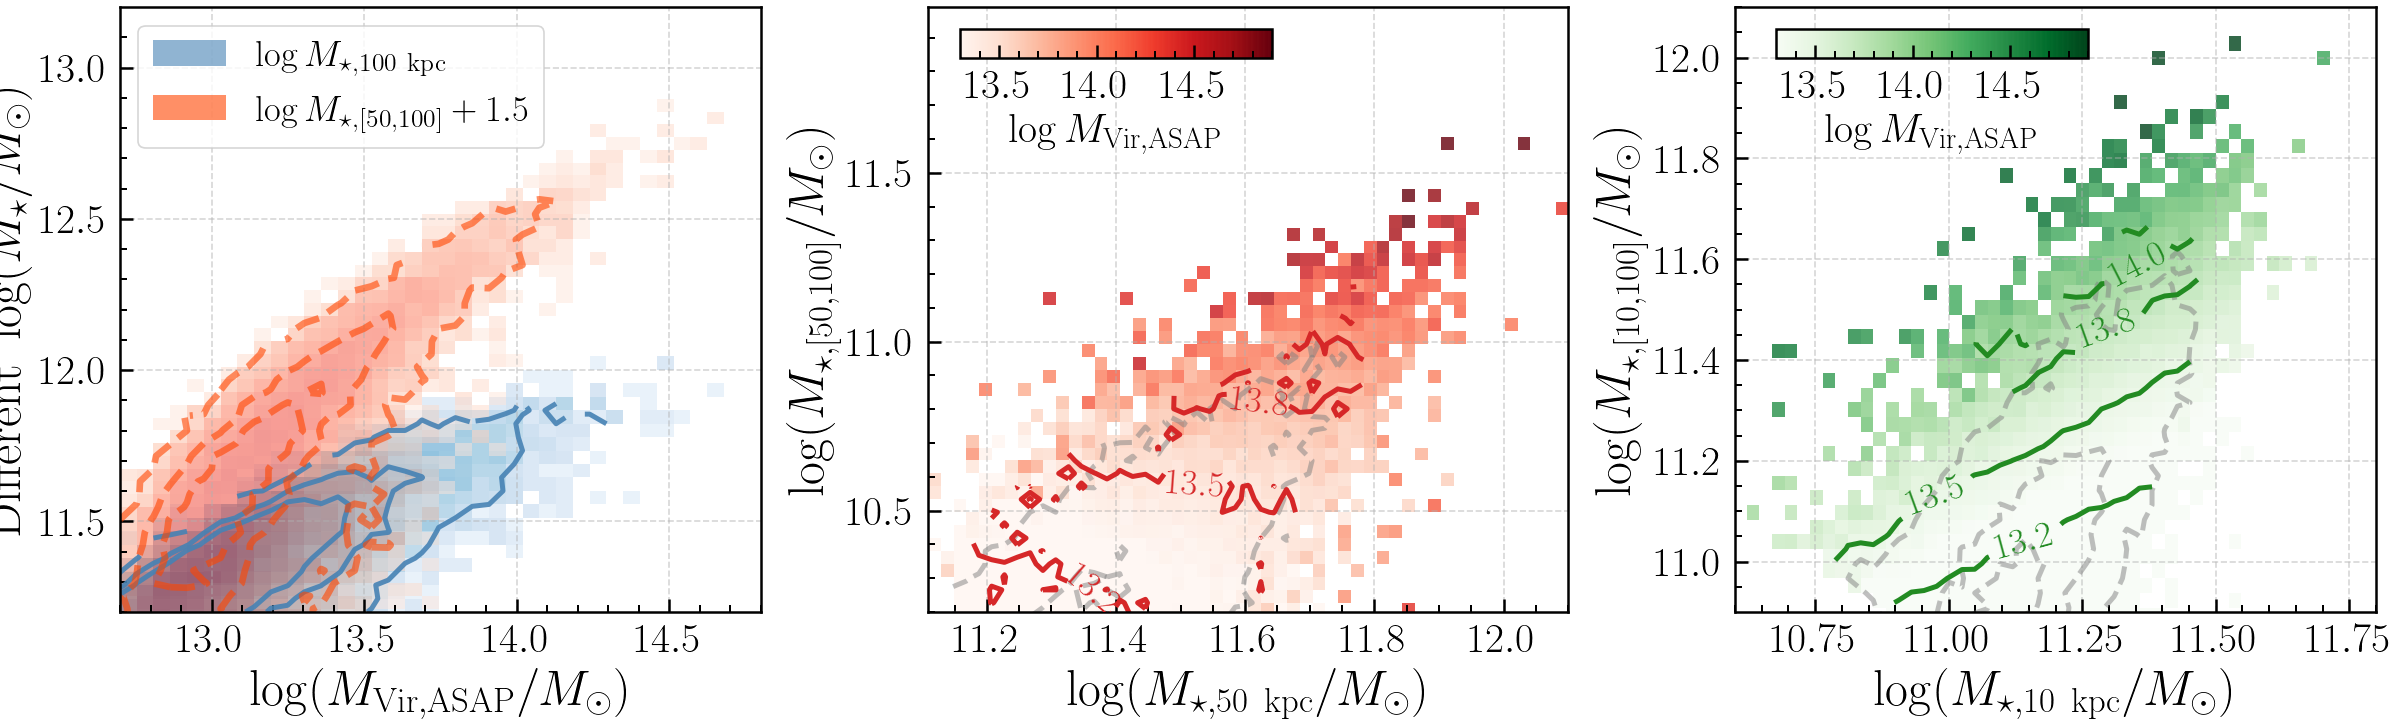
\includegraphics[width=\textwidth]{figure/topn_fig_12}
      \caption{
          Using the \mvir{} predicted by the \asap{} model, we explore the reason why the outer
          envelope stellar mass (e.g., \menve{50}{150}) out-perform the large aperture stellar mass
          such as the \maper{100} or \mmax{} as \mvir{} proxy.
          \textbf{Left}: relations between the \asap{}-predicted \mvir{} and two different stellar
          masses. Blue shaded region and solid-line contours are for the maximum 1-D stellar
          mass, \mmax{}. Red shaded region and dashed-line contours are for the outer envelope
          mass, \menve{50}{150}. Here colours indicate the number density of galaxies on this 2-D plane.
          \menve{} clearly displays tighter relation with the predicted \mvir{}.
          \textbf{Middle}: the 2-D plane of \mstar{} within 50 kpc (\maper{50}) v.s.
          \maper{50}{150} color coded by the \asap{}-predicted \mvir{}.
          Several iso-\mvir{} contours are used to highlight the relation between \mvir{} and
          \menve{50}{150}.
          \textbf{Right}: similar to the middle panel, here we show the \minn{} and \menve{10}{100}
          2-D plane color-coded by the \asap{}-predicted \mvir{}.
          Same set of iso-\mvir{} contours are used to compare with the middle panel.
      }
      \label{fig:outskirt_discussion}
  \end{figure*}
%% ---------------------------------------------------------------------------------------------- %%

%% ---------------------------------------------------------------------------------------------- %%
%% Discussion about the outer envelope mass
%% ---------------------------------------------------------------------------------------------- %%
\subsection{Why does the Outer Stellar Halo Trace Halo Mass?}
    \label{sec:outskirt_discussion}
    
    The key result of this work is that the outer envelope \mstar{} 
    (e.g., \menve{50}{100} or \menve{50}{150}) of massive galaxies is a better halo mass proxy 
    than the total \mstar{}.
    We do not calibrate the \mvir{}-\menve{50}{150} relation in this work.
    Instead, we demonstrate this using the \mvir{} predicted by the \asap{} model using \mstar{} 
    within two apertures (\citealt{Huang2020}).
    Although \masap{} is not a perfect \mvir{} proxy, it can faithfully represent the SHMR 
    when using large aperture \mstar{}.
    The left panel of Fig \ref{fig:outskirt_discussion} shows that the \masap{}--\menve{50}{150}
    relation indeed has steeper slope and lower scatter at high \masap{} end than the 
    \masap{}-\mmax{} relation.
    As demonstrated in \S \ref{sec:method} and Fig \ref{fig:theory_1}, this could explain the 
    better performance of outskirt \mstar{} in the \topn{} test.
    In the middle panel, we also visualize the \masap{} distribution over the \maper{50}
    and \menve{50}{150} 2-D plane.
    At \masap{}$>10^{13.6}$, the iso--\masap{} curve almost runs in parallel with the 
    \menve{50}{150}.
    When compared to the \maper{10}--\menve{10}{100} distributions in the right panel of 
    Fig \ref{fig:outskirt_discussion}, it reaffirms the finding that the outskirt
    \mstar{} at $R > 30$--50 kpc alone could be a great \mvir{} proxy, and adding \mstar{} 
    from inner region actually degrades its capability.
    
    This seemingly counter intuitive result can 
    be understood from the angle of the ``two-phase'' formation scenario of massive galaxies
    (e.g., \citealt{Oser2010, vanDokkum2010, Moster2020}).
    Under this picture, a massive galaxy consists of the stars formed within the halo of its main 
    progenitor at high redshift (\insitu{} component) and the accreted stars from repeated mergers 
    (\exsitu{} component).
    In \citet{Bradshaw2020}, the authors show the \mstar{} of the \exsitu{} component
    correlates with the halo mass much better than the \insitu{} component (see their Fig~9). 
    Although based on just one model, it is not surprising since the \exsitu{} component
    naturally reflects the halo assembly much better than the \insitu{} component.
    Both observations and hydro-simulations suggest that, at low redshift, the \exsitu{} 
    component dominate the outskirt of massive galaxies (e.g., \citealt{RodriguezGomez2016},
    \addref{}) and its fraction increases with both stellar and halo mass 
    (e.g., \addref{}).
    Therefore the outer envelope \mstar{} explored here could represent a substantial fraction
    of the \exsitu{} component and has the potential to be a promising \mvir{} proxy.
    
    Even with many details to be filled in, this result already shows interesting implications. 
    For instance, it suggests we could improve \asap{}-like models using an
    optimized choice of outer envelope \mstar{} 
    (see middle panel of Fig \ref{fig:outskirt_discussion}).
    Also, it provides additional motivation for us to try to ``decompose'' massive galaxies into
    \insitu{} and \exsitu{} component in real observation since the \exsitu{} \mstar{} could 
    be an even better \mvir{} proxy.
    Currently, this is still extremely challenging not only due to the lack of clear transition 
    feature between these two physical components in surface brightness distributions according
    to hydro-simulations (e.g., \citealt{Remus2021}), it is also because even the 
    state-of-the-art simulations still do not reproduce the stellar mass distribution of 
    low-$z$ massive galaxies perfectly (e.g., \citealt{Ardila2021}).
    We might need to search for better proxy of \exsitu{} \mstar{} than the outskirt \mstar{}
    with an arbitrary radial boundary. 
    Or we could try to find an alternative definition of ``\exsitu{}'' component that could 
    be constrained in real data easier than the current version.

    For low-$z$ massive galaxy clusters, there have been multiple works exploring the connection
    between the halo properties and the flux, shape, and radial profile of the intra-cluster
    light (ICL) -- essentially the extended outer envelope around the central galaxy (or the BCG)
    of the cluster (e.g., \citealt{Montes2018, Montes2019, Zhang2019b, Furnell2021, Kluge2021,
    SampaioSantos2021}.
    While several of them have demonstrates the tight correlation between the halo mass and 
    the stellar mass/luminosity of the BCG$+$ICL component\footnote{This is sometimes referred
    as the ``diffuse stellar light'' component following the definition in the Illustris-TNG
    simulation (e.g., \citealt{Zhang2019b, SampaioSantos2021}).} 
    (e.g., \citet{Zhang2019b, Kluge2021, SampaioSantos2021}), but whether the ICL alone is a 
    good halo mass proxy is still in debate (e.g., \citealt{Furnell2021}).
    As discussed in \citet{Huang2018b} and \citet{Kluge2020}, the definition of ICL is often 
    ambiguous and arbitrary, but the light between 50 to 150 kpc around a BCG is often considered 
    part of the ICL.
    Therefore our result helps confirm the correlation between the amount of ICL and halo mass,
    and also generalize it to all massive galaxies.

    We should also note that there is room to further improve the current outer envelope 
    \mstar{} measurement: the radial variation of \mlratio{} and projected 2-D shape could be 
    taken into account; more careful approach can be adopted to handle massive galaxies under 
    interaction or that are heavily blended with others.
    
%% ---------------------------------------------------------------------------------------------- %%
%% A ``perfect'' cluster finder?
%% ---------------------------------------------------------------------------------------------- %%
\subsection{Implication for Optical Cluster Finding}
    \label{sec:perfect_finder}
    
    On-going and future multi-band, deep, and wide imaging surveys provide exciting opportunities
    for identifying an unprecedentedly large samples of galaxy clusters within wide redshift and
    \mhalo{} ranges that can greatly advance cluster cosmology and the study of galaxy evolution
    in dense environment.
    Traditionally, cluster finders in the optical and NIR wavelength are mostly based on the 
    relation between \mvir{} and different measurements of the cluster richness.
    The \redm{} and \camira{} cluster finders rely on the number of quenched member galaxies
    on the red-sequence, while others use the over-density of galaxies within a narrow 
    photo-$z$ range (e.g., \citealt{Wen2021, Zou2021}).
    At the same time, although the SHMR at high \mstar{} end has been constrained in observation
    (e.g., \citealt{Leauthaud2012, Tinker2017, Kravtsov2018}), the \mstar{} of the cluster
    central galaxy (or the BCG) is still not considered a good proxy of \mvir{} given the shallow
    slope of the \mvir{}--\mstar{} relation.
    While there is physical reason behind this ``common knowledge'', we point out that it is also
    partially driven by poor photometric measurements of massive galaxies.
    
    As shown in \citet{Huang2018b}, photometry of massive galaxies can be heavily affected
    by over-subtracted sky background or over-deblending. 
    More importantly, the commonly adopted photometric models often cannot account for the
    surface brightness distribution of massive galaxies, and systematically under-estimate their
    luminosity and stellar mass.
    It is well documented now that the popular \cmodel{} photometry has these problems in both
    SDSS (e.g., \citealt{Bernardi2013}) and HSC survey (\citealt{Huang2018b}).
    Indeed, the \topn{} test clearly demonstrates that \mcmodel{} is a very poor \mvir{} proxy.
    Similar problems could also happen to \mstar{} based on small aperture photometry or 
    over-simplified model such as single-\ser{}.
    
    Meanwhile, the \topn{} tests also show that a properly measured \mstar{} based on either
    luminosity enclosed in a large aperture or within the outer envelope of massive galaxies has
    the potential to be a much better \mvir{} tracer.
    When evaluated by the \topn{} tests, their performance is comparable to the richness values
    measured by state-of-the-art cluster finders, and may even surpass them at relative low
    \mvir{}.
    In \citet{Rykoff2014}, the authors laid out seven ``golden rules'' for richness or 
    red-sequence based cluster finders.
    A \mstar{}-based \mvir{} proxy should naturally satisfy all of them.
    Therefore, it is promising to come up with new cluster finders that are based on different 
    \mstar{} measurements of the massive galaxies.
    Such cluster finders can open up new avenues of exploring massive dark matter halos.
    They may also own distinctive advantage over richness-based cluster finders.
    
    First and foremost, all aforementioned richness-based cluster finders suffer from 
    projection and orientation biases at different levels. 
    \song{Expand a little here, and discuss the DES result.} 
    %Note that the impact of projection effect on \dsigma{} profile shown in \citet{Sunayama2020}
    can not fully explain the differences we see.
    For \mstar{}-based cluster finder, both biases become much more limited since it 
    relies on measurements from a single galaxy.
    In \S \ref{sec:mstar_vs_richness}, we show that the \dsigma{} profiles of large aperture or
    outskirt \mstar{} \topn{} samples are consistent with certain samples of density-selected
    halos in N-body simulation.
    This could already demonstrate the less biased nature of \mstar{}-selected samples.

    Secondly, realistic mock catalogs of galaxies are essential for calibrating cluster 
    finders, understand their selection biases, and prepare them for cosmological applications.
    However, despite the recent progress (e.g., \citealt{DeRose2019, Hearin2020}), the
    red-sequence or the colour distributions of galaxies in general has been notoriously
    difficult to model using either semi-analytic models or hydro-simulation (\addref{}).
    %To have an realistic colour distribution essentially requests the correct star formation
    %history, chemical evolution history, and stellar population model.
    %None of these is a trivial task. 
    It is also difficult to account for all the systematics that affect the colour measurements
    into the mock catalog.
    On the other hand, it is relatively easier to calibrate the \mstar{} measurements when the
    same definition is adopted in both observation and simulation/model (e.g.,
    \citet{Ardila2021}).
    And, to reproduce the richness-selected clusters in simulations or models, a realistic 
    population of cluster members is also necessary. This is also not a trivial task.
    Meanwhile, it is conceptually easier to reproduce the observed properties of just the 
    massive central galaxies (e.g., \citealt{Moster2020}).
    To utilized the \mstar{}-based ``cluster finder'', we do need to account for the massive
    satellite galaxies (see \ref{sec:satellite}), but this should be an easier problem to deal
    with using modern galaxy--halo connection models or semi-analytic/empirical models.
    We should note that, to take advantage of the outer envelope \mstar{} as a better
    \mstar{}-based \mvir{} proxy, we still need to understand how to model the \mstar{} 
    profile of massive galaxies or find a reliable proxy of the \exsitu{} component.
    These 

    In addition, \mstar{}-based finder may have advantage at higher redshift where the 
    red-sequence becomes less significant or intrinsically wider in massive halos.
    Central galaxies with on-going star-formation (blue BCGs) is another issue for 
    red-sequence cluster finders. 
    It is a minor issue at low redshift (e.g., \citealt{Rykoff2014}), but could become
    more important at higher redshift.
    \mstar{}-based finder should be able to handle it with appropriate priors in the
    SED fitting process

    We believe the advantages discussed above means the \mstar{}-based cluster finders
    not only can help us understand the systematics of richness-based cluster finders,
    they can also provide important additional constraints of cosmology and 
    galaxy-halo connection models.


%% ---------------------------------------------------------------------------------------------- %%
%% Summary
%% ---------------------------------------------------------------------------------------------- %%
\section{Summary and Conclusions}
    \label{sec:summary}

%% ---------------------------------------------------------------------------------------------- %%
%% Background and review of the paper
%% ---------------------------------------------------------------------------------------------- %%
    In this work, we show that the comparison of stacked \dsigma{} profiles around proposed
    cluster centers at fixed number density can be used as a method to inter-compare cluster
    finding methods (\S \ref{sec:topn_intro} and \S \ref{sec:comp_scatters}).
    Using cosmological simulations and a simple \mvir{}-observable model that only
    considers a Gaussian scatter around the mean relation, we show that we can estimate the
    scatter of \mvir{} at a fixed value for the observable (\S \ref{sec:estimate_scatter}).
    In practice, this \topn{} test provides us a way to evaluate the performance of different
    \mvir{} proxies (\S \ref{sec:proxies}) used to identify massive halos, infer the
    galaxy-halo connection, and study galaxy evolution.

    Taking advantage of the deep imaging data and unprecedented lensing capability of the HSC
    SSP survey (\S \ref{sec:hsc}), we evaluate different \mstar{}-based and richness-based
    \mvir{} proxies for massive galaxies and halos at $0.2 < z < 0.5$.
    Within this redshift range, we carefully extract 1-D surface mass density profiles (\S
    \ref{sec:1d_prof}) for a large sample of massive galaxies (\logmaper{100}$\geq 11.5$, \S
    \ref{sec:galaxy_sample}), and use these profiles to measure the \mstar{} enclosed within
    various elliptical apertures (\S \ref{sec:maper}) and outer envelopes (\S
    \ref{sec:menvelope}).
    We also consider two popular red-sequence cluster finders: \redm{}
    (\S \ref{sec:cluster_redmapper}) and \camira{} (\S \ref{sec:cluster_camira}) and include
    their richness measurements in the \topn{} tests.
    After splitting all selections into four number density bins (\S \ref{sec:binning}) and
    measuring the \dsigma{} profiles (\S \ref{sec:dsigma} and Appendix \ref{app:dsigma_detail})
    of different proxies in each bin, we
    1) estimate and compare the \sigmvir{} values, and evaluate their performance as \mvir{}
    proxies;
    2) investigate whether their \dsigma{} profiles are consistent with an observable that has
    a log-linear relationship with \mvir{} with Gaussian scatter.
    The main results from these tests are:

%% ---------------------------------------------------------------------------------------------- %%
%% Main conclusions
%% ---------------------------------------------------------------------------------------------- %%
    \begin{itemize}

        \item While satellite galaxies do not have a strong impact on the stacked \dsigma{}
            profile of the highest \mstar{} samples (due to a lower satellite fraction),
            they leave a distinctive and visible trace toward the lower-\mstar{} end (\S
            \ref{sec:satellite}). We need to model their contribution before we can fully realize
            the potential of any \mstar{}-based \mvir{} proxy.

        \item \mstar{} based on \cmodel{} or any other default photometry of galaxies from
            a generic data reduction pipeline is often not a good \mvir{} proxy for massive galaxies
            (see \S \ref{sec:m100_cmodel} and Figure \ref{fig:m100_cmod}).
            \cmodel{} does not accurately account for the flux in massive galaxies' extended
            stellar halo; the very flux that has the tightest connection with the underlying \mvir{}.
            We caution against the use of \cmodel{}-like photometry in the study of the galaxy-halo
            connection of massive galaxies in the future.

        \item Compared to \mcmodel{}, the \mstar{} enclosed in a large aperture such as \maper{100}
            is a much better \mvir{} proxy (\S \ref{sec:m100_cmodel}; Figure \ref{fig:m100_cmod}).
            In addition to the smaller \sigmvir{} value in each bin, the
            \mvir{}-observable scaling relation with Gaussian scatter model can adequately
            describe the stacked \dsigma{} profile around \maper{100} selected clusters.
            However, the performance evaluated using the inferred \sigmvir{} is not on par with
            richness-based red-sequence cluster finders such as \redm{} and
            \camira{} (Figure \ref{fig:scatter_trend}) except in the very low richness regime
            (e.g., $\lambda_{\rm redMaPPer} \leq 10$).

        \item \mstar{} in the outer envelope of massive galaxies such as \menve{50}{150} is
            a promising \mstar{}-based \mvir{} proxy (\S \ref{sec:m100_outskirt};
            Figure \ref{fig:m100_mout}).
            The outer envelope \mstar{}-selected samples show \dsigma{} profiles that
            are perfectly fit by our ``scatter-only'' model, and also have lower \sigmvir{}
            values than any large aperture \mstar{} samples.
            The performance of \menve{50}{150} approaches that of richness-based proxies even at
            the high-\mvir{} end (Figure \ref{fig:scatter_trend}).
            This result strongly supports the idea that the outer envelope of massive galaxies
            has a better connection with the assembly of the dark matter halo, presumably because
            it is dominated by \exsitu{} stars.
        
        \item While both richness-based \mvir{} proxies (\redm{} and \camira{}) have
            impressively low inferred \sigmvir{} values at $\lambda_{\rm redMaPPer} > 10$ or
            $N_{\rm CAMIRA} > 10$, the \dsigma{} profiles of their selections do not show the
            expected shape.
            Their profiles are not consistent with either the ``scatter-only'' model, or \mstar{}
            selected samples (see Figure \ref{fig:mout_richness}).
            Instead, their \dsigma{} profiles have enhanced amplitudes around $R\sim
            1$-2 Mpc and suppressed inner profiles at $R < 1$ Mpc compared to the \mstar{}-based
            ones in the same number density bin (\S \ref{sec:mstar_vs_richness} and Figure
            \ref{fig:richness_residual}).
            These results indicate that the richness-based \mvir{} proxies have additional
            systematics (e.g., mis-centering, projection effect) that need to be accounted for.
            
    \end{itemize}

%% ---------------------------------------------------------------------------------------------- %%
%% Future directions
%% ---------------------------------------------------------------------------------------------- %%
    % Future direction
    Based on these results, we plan to further pursue the idea of using \mstar{}-based
    \mvir{} proxies to study the galaxy-halo connection and cosmology.
    Recent HSC data releases (\texttt{S20A} or \texttt{PDR3} in 2021) have increased sky
    coverage to $> 600$ deg$^2$, four times larger than the current sample.
    Not only would these larger samples improve the statistical uncertainty of the \topn{} tests,
    they would also enable us to explore the high-\mvir{} regime much better than the
    broad richness bin used here.
    Moreover, the new releases come with improved background subtraction that can greatly help in
    probing the outer profile of massive galaxies.
    We are also working on an improved outer envelope \mstar{} measurement using a more accurate
    \mlratio{} and a more sophisticated modeling approach.
    On the theoretical side, we will use state-of-the-art hydro-simulations and
    semi-empirical models to investigate the connection between the outer envelope of massive
    galaxies and the assembly history of their dark matter halo.
    At the same time, it would be interesting to compare the cluster samples selected by 
    richness- and \mstar{}-based methods.
    In addition to the selection biases of different methods, it may also help us investigate the
    distribution of halo properties at high-\mvir{} end.
    Comparing the \mstar{}-selected clusters to the ones identified by other multi-wavelength
    methods that are not sensitive to the projection effect (e.g., X-ray observation) will be
    useful to further calibrate the \mstar{}-based cluster finder.

    More importantly, as outlined in \citet{Bradshaw2020}, we suggest that a ``hybrid''
    cluster finder that combines the advantages of richness- and \mstar{}-based \mvir{} 
    proxies is possible by simply combining the \mstar{} of the central galaxy and 
    a few (e.g., top 2 or 3) massive satellite galaxies.
    Such a ``Cen$+N$'' method could be an excellent \mvir{} proxy, with low 
    \sigmvir{} values in a given number density bin while also suffering minimally from
    systematics such as projection effects.
    
    Both the \mstar{}-based and the ``Cen$+N$'' methods require accurate identification
    of massive satellite galaxies.
    This is a challenging task when using photo-$z$ from imaging surveys.
    Spectroscopic surveys such as DESI (e.g., \citealt{DESI2016}) will greatly improve the 
    situation.
    Using images from the The DECam Legacy Survey (DECaLS, e.g., \citealt{Dey2019})\footnote{
        \url{https://www.legacysurvey.org/}
    }, we will measure large aperture and outer envelope \mstar{} of $z<0.5$ massive galaxies 
    out to $\sim 100$ kpc (e.g., Li et al. in prep.).
    When combined with their DESI spec-$z$ in the next few years, this much larger DECaLS ($\sim
    9000$ deg$^2$) survey will provide us an ideal sample to constrain galaxy-halo connection
    models.
    We will extend our \topn{} tests to include group/cluster catalogs for DECaLS 
    (e.g., \citealt{Yang2020, Zou2021}), and apply our ``Cen$+N$'' method to define a 
    sample of massive halos that are suitable for unbiased cosmological analysis.

%% ---------------------------------------------------------------------------------------------- %%
%% Acknowledgements
%% ---------------------------------------------------------------------------------------------- %%
\section*{Acknowledgements}

  % Personal
  %\todo{The authors would like to thank XXX for useful discussions and suggestions.}

  % NSF funding
  This material is based upon work supported by the National Science Foundation under
  Grant No. 1714610.

  % KITP
  The authors acknowledge support from the Kavli Institute for Theoretical Physics.
  This research was also supported in part by National Science Foundation under Grant
  No. NSF PHY11-25915 and Grant No. NSF PHY17-48958

  % AL's funding
  We acknowledge use of the lux supercomputer at UC Santa Cruz, funded by NSF MRI grant AST
  1828315. AL is supported by the U.D Department of Energy, Office of Science, Office of High
  Energy Physics under Award Number DE-SC0019301. AL acknowledges support from the David and
  Lucille Packard foundation, and from the Alfred .P Sloan foundation.

  % HSC part
  The Hyper Suprime-Cam (HSC) collaboration includes the astronomical communities of
  Japan and Taiwan, and Princeton University.  The HSC instrumentation and software were
  developed by National Astronomical Observatory of Japan (NAOJ), Kavli Institute
  for the Physics and Mathematics of the Universe (Kavli IPMU), University of Tokyo,
  High Energy Accelerator Research Organization (KEK), Academia Sinica Institute
  for Astronomy and Astrophysics in Taiwan (ASIAA), and Princeton University.
  Funding was contributed by the FIRST program from Japanese Cabinet Office,  Ministry
  of Education, Culture, Sports, Science and Technology (MEXT), Japan Society for
  the Promotion of Science (JSPS), Japan Science and Technology Agency (JST), Toray
  Science Foundation, NAOJ, Kavli IPMU, KEK, ASIAA, and Princeton University.

  % SDSS part
  Funding for SDSS-III has been provided by Alfred P. Sloan Foundation, the
  Participating Institutions, National Science Foundation, and U.S. Department of
  Energy. The SDSS-III website is http://www.sdss3.org.  SDSS-III is managed by the
  Astrophysical Research Consortium for the Participating Institutions of the SDSS-III
  Collaboration, including University of Arizona, the Brazilian Participation Group,
  Brookhaven National Laboratory, University of Cambridge, University of Florida, the
  French Participation Group, the German Participation Group, Instituto de Astrofisica
  de Canarias, the Michigan State/Notre Dame/JINA Participation Group, Johns Hopkins
  University, Lawrence Berkeley National Laboratory, Max Planck Institute for
  Astrophysics, New Mexico State University, New York University, Ohio State University,
  Pennsylvania State University, University of Portsmouth, Princeton University, the
  Spanish Participation Group, University of Tokyo, University of Utah, Vanderbilt
  University, University of Virginia, University of Washington, and Yale University.

  % Pan-STARRS1 part
  The Pan-STARRS1 surveys (PS1) have been made possible through contributions of
  Institute for Astronomy; University of Hawaii; the Pan-STARRS Project Office;
  the Max-Planck Society and its participating institutes: the Max Planck Institute
  for Astronomy, Heidelberg, and the Max Planck Institute for Extraterrestrial Physics,
  Garching; Johns Hopkins University; Durham University; University of Edinburgh;
  Queen's University Belfast; Harvard-Smithsonian Center for Astrophysics; Las
  Cumbres Observatory Global Telescope Network Incorporated; National Central
  University of Taiwan; Space Telescope Science Institute; National Aeronautics
  and Space Administration under Grant No. NNX08AR22G issued through the Planetary
  Science Division of the NASA Science Mission Directorate; National Science
  Foundation under Grant No. AST-1238877; University of Maryland, and Eotvos
  Lorand University.

  % LSST software
  This research makes use of software developed for the Large Synoptic Survey
  Telescope. We thank the LSST project for making their code available as free
  software at http://dm.lsstcorp.org.

  % SMDPL simulation
  The CosmoSim database used in this research is a service by the Leibniz-Institute for
  Astrophysics Potsdam (AIP).
  The MultiDark database was developed in cooperation with the Spanish MultiDark
  Consolider Project CSD2009-00064.

  % Software
  This research made use of:
  \href{http://www.stsci.edu/institute/software_hardware/pyraf/stsci\_python}{\texttt{STSCI\_PYTHON}},
      a general astronomical data analysis infrastructure in Python.
      \texttt{STSCI\_PYTHON} is a product of the Space Telescope Science Institute,
      which is operated by Association of Universities for Research
      in Astronomy (AURA) for NASA;
  \href{http://www.scipy.org/}{\texttt{SciPy}},
      an open source scientific tool for Python (\citealt{SciPy});
  \href{http://www.numpy.org/}{\texttt{NumPy}},
      a fundamental package for scientific computing with Python (\citealt{NumPy});
  \href{http://matplotlib.org/}{\texttt{Matplotlib}},
      a 2-D plotting library for Python (\citealt{Matplotlib});
  \href{http://www.astropy.org/}{\texttt{Astropy}}, a community-developed
      core Python package for astronomy (\citealt{AstroPy});
  \href{http://scikit-learn.org/stable/index.html}{\texttt{scikit-learn}},
      a machine-learning library in Python (\citealt{scikit-learn});
  \href{https://ipython.org}{\texttt{IPython}},
      an interactive computing system for Python (\citealt{IPython});
  \href{https://github.com/kbarbary/sep}{\texttt{sep}}
      Source Extraction and Photometry in Python (\citealt{PythonSEP});
  \href{https://jiffyclub.github.io/palettable/}{\texttt{palettable}},
      colour palettes for Python;
  \href{http://dan.iel.fm/emcee/current/}{\texttt{emcee}},
      Seriously Kick-Ass MCMC in Python;
  \href{http://bdiemer.bitbucket.org/}{\texttt{Colossus}},
      COsmology, haLO and large-Scale StrUcture toolS (\citealt{Colossus}).

%% ---------------------------------------------------------------------------------------------- %%
%% References
%% ---------------------------------------------------------------------------------------------- %%
\bibliographystyle{mnras}
\bibliography{topn}

%% ---------------------------------------------------------------------------------------------- %%
%% Appendix Section
%% ---------------------------------------------------------------------------------------------- %%

\appendix

%% ---------------------------------------------------------------------------------------------- %%
%% Derive the DSigma profile
%% ---------------------------------------------------------------------------------------------- %%
\section{Derivation of $\Delta\Sigma$}
    \label{app:dsigma_detail}

    Here we walk through the derivation of the final \dsigma{} profile used in the \topn{} test.
    As mentioned in \S \ref{sec:dsigma}, we adopt a slightly modified version of the methodology
    from \citet{Singh2017} to measure the excess surface mass density (ESD or \dsigma{}) profiles
    around massive galaxies or clusters.
    This method emphasizes the importance of subtracting lensing signals around large number of
    random positions from the signals for real lenses to achieve unbiased measurement.
    The \dsigma{} signal at a physical radius $R$ is:

    \begin{equation}
        {\Delta\Sigma}_{\rm LR}(R) =
        f_{\rm bias}({\Delta\Sigma}_{\mathrm{L}}(R) - {\Delta\Sigma}_{\mathrm{R}}(R))
        \label{eq:ds1}
    \end{equation}

    Here, $L$ indicates measurements for the lens galaxies while $R$ is for random positions.
    For each \dsigma{} profile, we use a set of $1.5 \times 10^5$ random points whose redshift
    distribution is matched to the lenses.
    The number of random points is at least 100 time larger than the largest \topn{} sample.
    The \dsigma{} profile around lenses is:

    \begin{equation}
        {\Delta\Sigma}_{\rm L}(R) = \frac{1}{2 \mathcal{R}(R) [1+\mathcal{K}(R)]}
            \frac{\Sigma_{\rm Ls} w_{\rm Ls} \gamma_{t}^{(\rm Ls)}
            \Sigma_{\rm crit}^{(\rm Ls)}}{\Sigma_{\rm Ls} w_{\rm Ls}}
        \label{eq:ds2}
    \end{equation}

    \noindent where $\gamma_{t}$ is the tangential shear component, $\Sigma_{\rm crit}$ is the
    critical surface density, $w_{\rm Ls}$ is the weight used for each lens-source pair.
    Following the calibration strategy outlined in \citet{HSC-WLCALIB}, we also include
    the shear responsivity factor $\mathcal{R}(R)$ and the correction for the multiplicative
    shear bias $[1+\mathcal{K}(R)]$.
    Here $\Sigma{\rm Ls}$ represents the summation over all lens-source pairs.
    We perform the same measurements for random points, so replacing L with R in
    Equation \ref{eq:ds2} will form the estimator for randoms.

    The critical surface density is:

    \begin{equation}
        \Sigma_{\rm crit}=\frac{c^2}{4\pi G} \frac{D_A(z_s)}{D_A(z_l) D_A(z_l, z_s) (1+z_l)^2}
        \label{eq:sigcrit}
    \end{equation}

    \noindent where $D_A(z_L)$, $D_A(z_s)$, and $D_A{z_L, z_s}$ represent the angular diameter
    distances to the lens, source, and the distance between the lens-source pair.

    The weight applied to each lens-source pair is described by:

    \begin{equation}
        w_{\rm Ls} = \frac{\Sigma_{\rm crit}^{-2}}{\sigma^2_{e, {\rm Ls}} + \sigma^2_{\rm rms}}
            \equiv \frac{\Sigma_{\rm crit}^{-2}}{\sigma^2_{{\rm Ls}}}
        \label{eq:weight}
    \end{equation}

    \noindent where $\sigma_{\rm rms}$ represents the intrinsic shape dispersion while
    $\sigma_{e, \rm Ls}$ is the per-component shape measurement error.

    Meanwhile, the shear responsivity factor is defined by:

    \begin{equation}
        \mathcal{R}(R) = 1 - \frac{\Sigma_{\rm Ls} w_{\rm Ls} \sigma^2_{e, {\rm Ls}}}{\Sigma_{\rm Ls} w_{\rm Ls}}
        \label{eq:rfactor}
    \end{equation}

    \noindent And the multiplicative shear bias correction is defined as:

    \begin{equation}
        \mathcal{K}(R) = \frac{\Sigma_{\rm Ls} w_{\rm Ls} m_{\rm s}}{\Sigma_{\rm Ls} w_{\rm Ls}}
        \label{eq:kfactor}
    \end{equation}

    \noindent where $m_{\rm s}$ is multiplicative shear bias value for each source.
    The shape catalog provides estimates of $\sigma_{\rm rms}$, $\sigma_{e, \rm Ls}$, and $m_{\rm
    s}$, while \citet{HSC-WLCALIB} provides in-depth discussion of these calibration related
    issues.

    In difference with \citet{Singh2017}, we do not use boost factor to account for the photo-$z$
    dilution effect.
    Following the strategy in \citet{Leauthaud2017}, we develop a correction
    factor, $f_{\rm bias}$, to account for it.
    We define $f_{\rm bias}$ as the ratio between the \dsigma{} profile calculated using
    the real redshift and the one using photo-$z$ from the COSMOS photo-$z$ calibration
    catalog\footnote{The catalog can be found here:
    https://hsc-release.mtk.nao.ac.jp/doc/index.php/s17a-wide-cosmos/}.

    In practice, it is estimated based on:

    \begin{equation}
        f_{\rm bias} = \frac{\sum_{\rm Ls} w_{\rm Ls} w_{\rm sys}
            \left(\Sigma_{{\rm crit, T}} / \Sigma_{{\rm crit, P}} \right)}{
            \sum_{\rm Ls} w_{\rm Ls} w_{\rm sys} \Sigma^{-2}_{\rm crit, P}}
        \label{eq:fbias}
    \end{equation}

    based on the photo-$z$ calibration sample in the COSMOS field for
    such purpose
    (e.g., \citealt{Mandelbaum2008, Nakajima2012, Leauthaud2017}).

    As for the $f_{\rm bias}$,

    \noindent where $\Sigma_{{\rm crit, T}}$ is the critical surface density estimated using the
    ``true'' redshift in the calibration catalog (can be spec-$z$ or COSMOS 30-band photo-$z$),
    while $\Sigma_{{\rm crit, P}}$ is the one using \texttt{frankenz} photo-$z$.
    $w_{\rm sys}$ is the systematic photo-$z$ weight in the calibration catalog that matches the
    color-magnitude distribution of the COSMOS photo-$z$ calibration catalog to the same
    distribution of the source catalog (e.g., \citealt{Mandelbaum2008, Nakajima2012}).
    Note that the estimator shown here is different from the ones in \citet{Leauthaud2017} and
    \citet{Speagle2019}, and it accounts for the photo-$z$ dilution effect more accurately.
    The $f_{\rm bias}$ level for galaxies in our sample is general very low ($\sim 1$-2\%).

    To estimate the covariance matrix of a \dsigma{} profile, we use both jackknife and
    bootstrap resampling method.
    For the jackknife case, we assign lens and randoms into the same 45 jackknife regions with
    similar area around 2.5 \sqdeg{} and regular shapes.
    The covariance matrix from the jackknife resampling is:

    \begin{equation}
        \mathrm{Var}_{\rm Jk}(\widehat{\Delta\Sigma}) = \frac{N_{\rm Jk} - 1}{N_{\rm Jk}} \sum\limits_{i=1}^{N_{\rm Jk}} (\Delta\Sigma_{i} - \overline{\Delta\Sigma})^2
    \end{equation}

    \noindent here $N_{\rm Jk}=45$, $\Delta\Sigma_{i}$ represents the \dsigma{} profile from each
    Jackknife region, and $\overline{\Delta\Sigma}$ is the mean profile of all regions.

    For the \topn{} test, the small sample size in Bin 1 \& 2 sometimes make it difficult to assign
    jackknife regions. Therefore we also calculate the covariance matrix using bootstrap resampling
    with $N_{\rm Bt}=5000$ iterations:

    \begin{equation}
        \mathrm{Var}_{\rm Bt}(\widehat{\Delta\Sigma}) = \frac{1}{N_{\rm Bt} - 1} \sum\limits_{i=1}^{N_{\rm Bt}} (\Delta\Sigma_{i, \rm Bt} - \overline{\Delta\Sigma})^2
    \end{equation}

    \noindent The two methods provide consistent measurements of covariance matrix.


%% ---------------------------------------------------------------------------------------------- %%
%% Figure: Demonstrate the scatter matching process.
%% ---------------------------------------------------------------------------------------------- %%
  \begin{figure*}
      \centering
      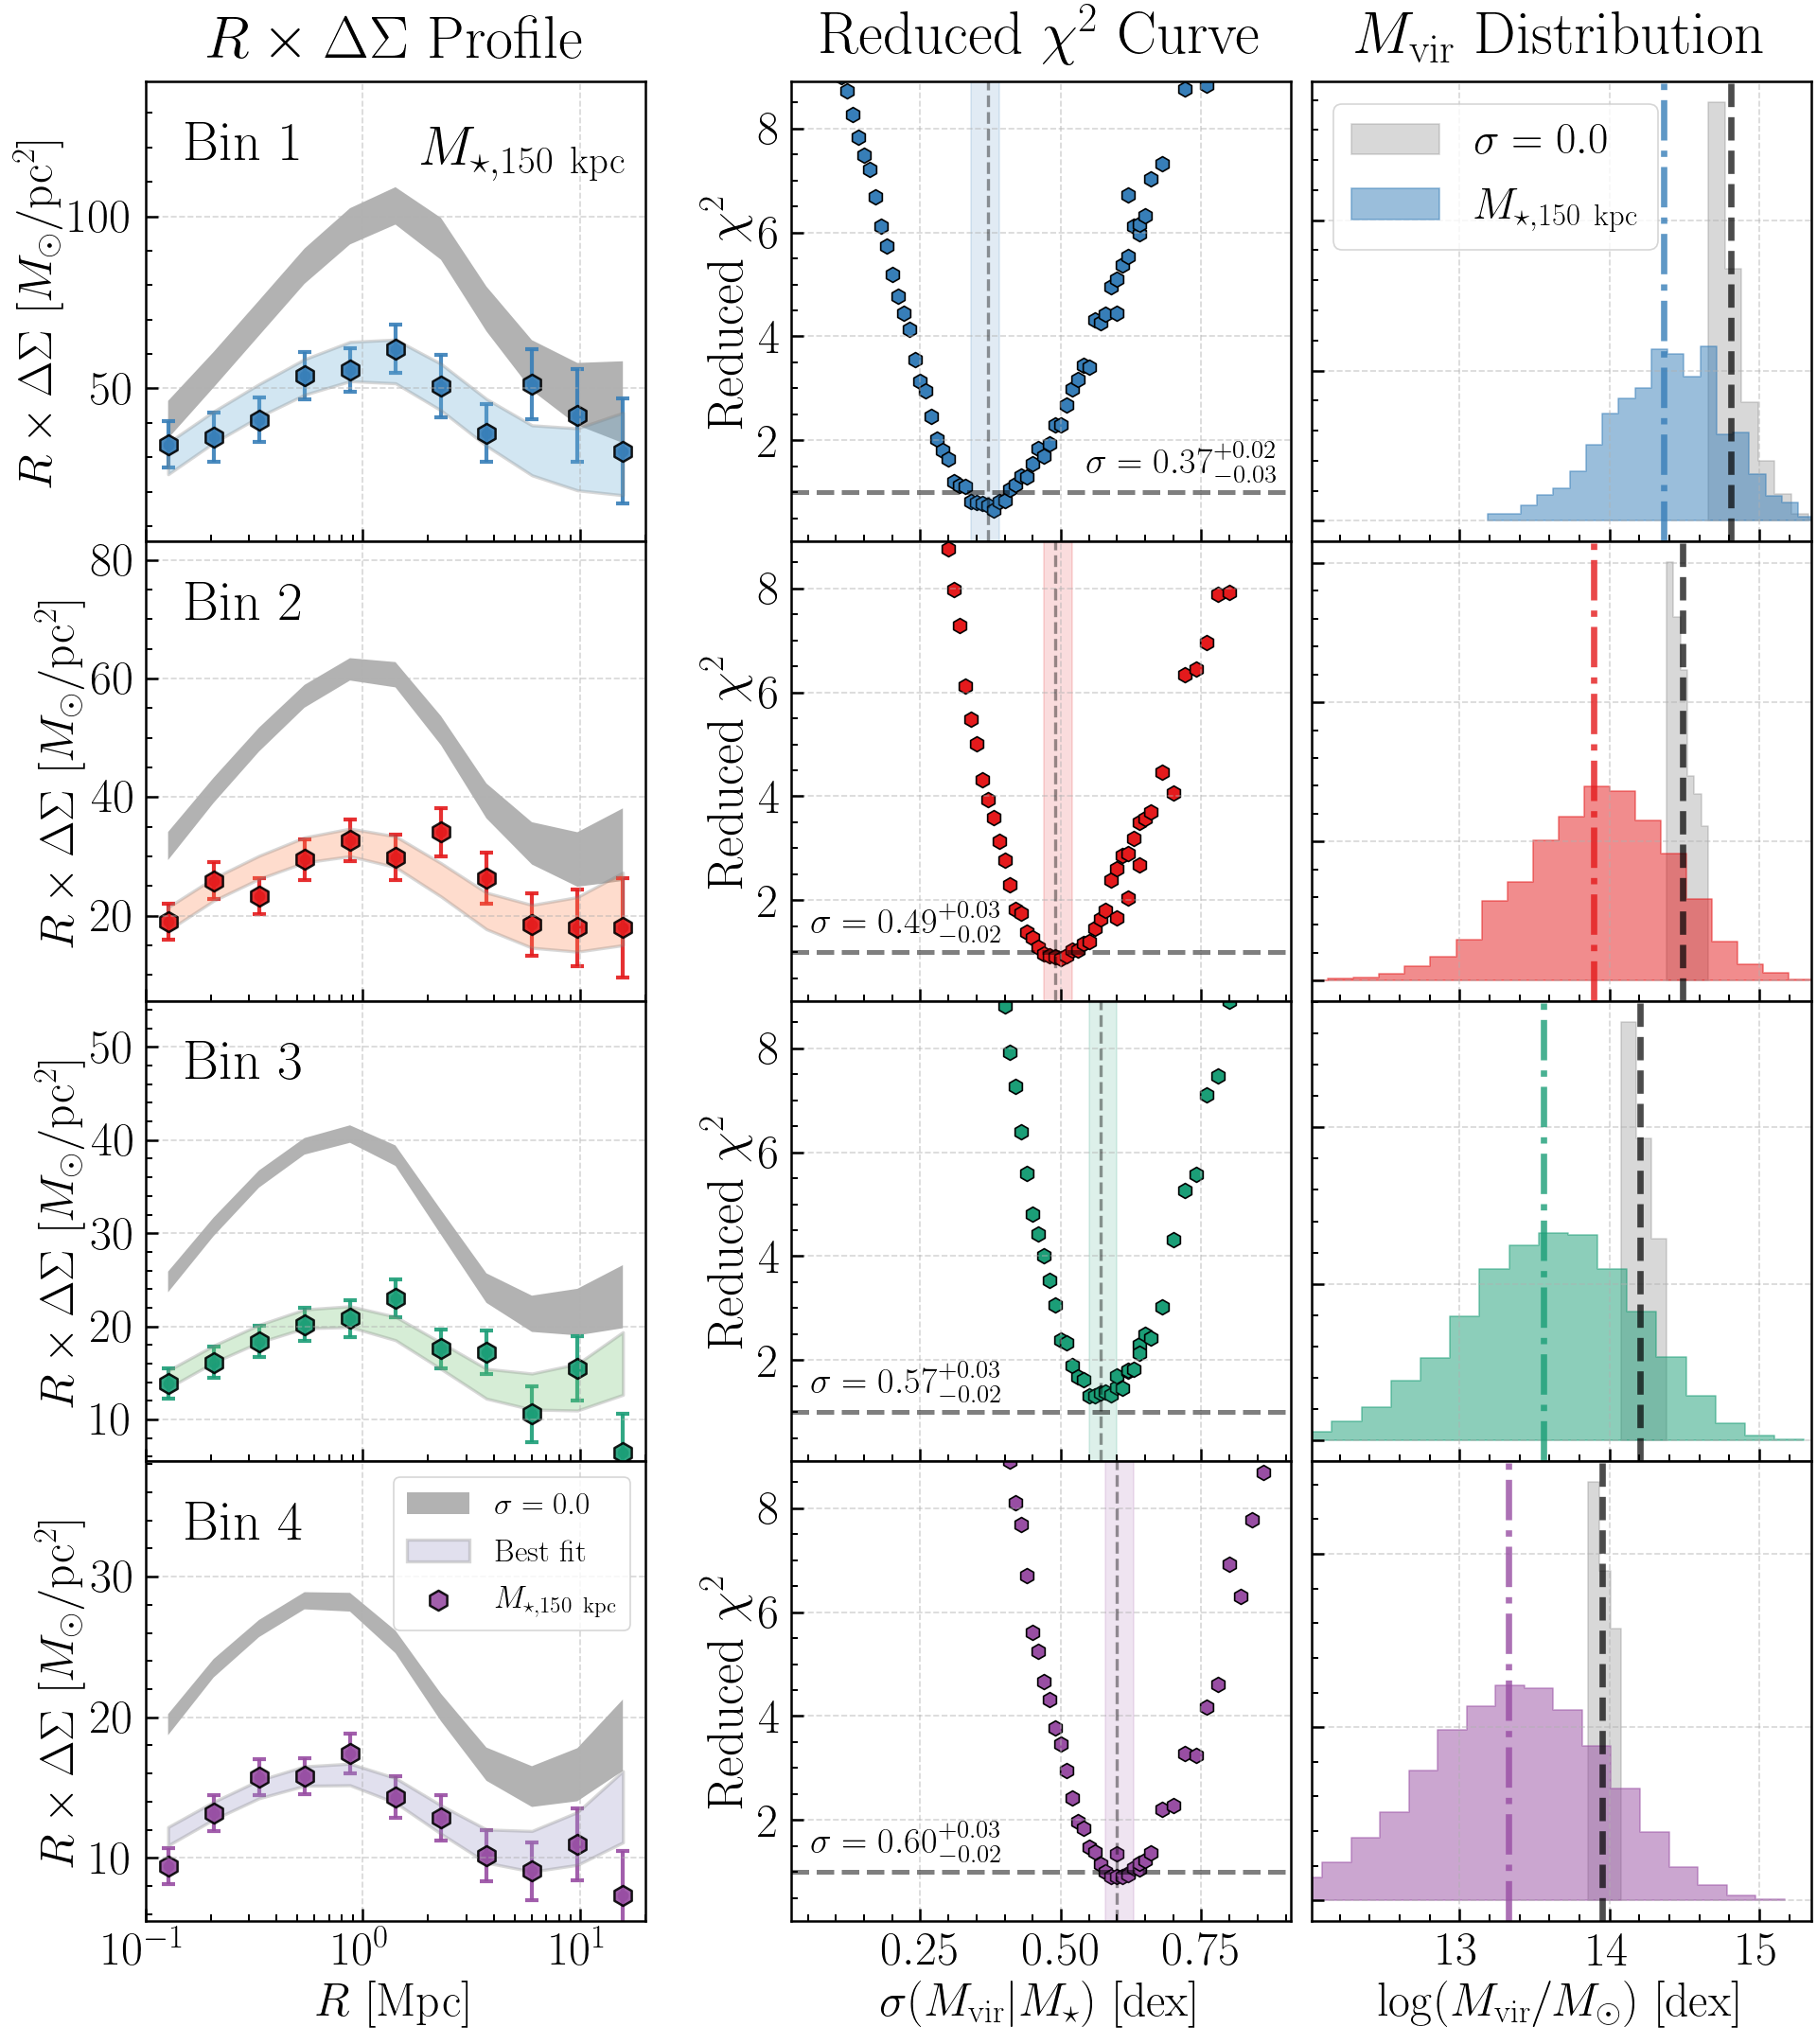
\includegraphics[width=\textwidth]{figure/topn_fig_appendix_1}
      \caption{
          Illustration of the scatter-matching process in the four \topn{} bins using the
          \maper{150} as an example.
          \textbf{Left} column shows the observed \rdsigma{} profiles (solid hexagon), the best-fit
          profiles using \mdpl2{} simulation (shaded regions with similar colours), and the
          lensing profiles of the ``perfect'' \topn{} sample.
          The uncertainties of the model lensing profiles are inflated to match the expected
          statistical uncertainties of the volume occupied by the HSC data.
          \textbf{Middle} column shows the reduced $\chi^{2}$ curve of the fitting process.
          A horizontal dashed-line highlights where $\chi^{2}=1$.
          The vertical dashed-line and the shaded region show the best-fit scatter value and the
          associated uncertainty. We also display these values on the figure.
          \textbf{Right} column shows the best-fit \mvir{} distributions in each bin predicted
          by the \mdpl2{} simulation (colored histograms; dot-dashed lines label the average
          \mvir{} values).
          We also compare them with the ``true'' \mvir{} distributions in each number density bin
          (grey histograms; grey dashed-lines label the average \mvir{} values).
      }
      \label{fig:fitting}
  \end{figure*}
%% ---------------------------------------------------------------------------------------------- %%

%% ---------------------------------------------------------------------------------------------- %%
%% More on the method of profile matching
%% ---------------------------------------------------------------------------------------------- %%
\section{Matching \dsigma{} profiles}
    \label{app:fitting}

    As described in \S \ref{sec:estimate_scatter}, we estimate the \sigmh{} value
    from an observed \dsigma{} profile from the \topn{} test through matching it to a densely
    sampled grid of model \dsigma{} profiles that cover a wide range of \sigmh{}
    values.
    For each pair of observed and predicted \dsigma{} profiles, we define a simple $\chi^2$
    statistic (Equation \ref{eq:chi2}) to describe the ``similarity'' between them.

    In Figure \ref{fig:fitting}, we use the \topn{} result for \maper{150} stellar mass as example
    to visualize the ``scatter matching'' procedure, which produce a well-behaved reduced $\chi^2$
    curves with a clear minimum.
    For \maper{150}, the reduced $\chi^2$ values in all four \topn{} bins are reasonably close
    to 1.0 ([0.65, 0.88, 1.31, 0.90]).
    In line with this impression, the left panels show that the best-fit ``scatter only'' \dsigma{}
    profile is fully consistent with the observed one.
    As discussed in \S \ref{sec:mstar_vs_richness}, this is not always the case (see
    Figure \ref{fig:richness_residual}).
    However, even when the best-fit model is not satisfying (e.g., reduced $\chi^2 >2$), we still
    estimate the ``best-fit'' \sigmh{} value.

    Since we only calculate the $\chi^2$ on a grid of \sigmh{} values and the statistical
    uncertainties of the predicted \dsigma{} profiles cannot be completely ignored, we did not
    just report the \sigmh{} value with the lowest $\chi^2$.
    Instead, we interpolate the normalized cumulative distribution of the likelihood $\equiv
    \exp{(-0.5 \times \chi^2)}$ to derive the \sigmh{} at 50th percentile as the ``best-fit''
    scatter value.
    We estimate the 1-$\sigma$ uncertainty range in the same way.

    We should note that the choice of covariance matrix (Jackknife v.s. bootstrap) does not
    affect any results of this work.
    We also attempted to include the uncertainties of the predicted \dsigma{} profile to the
    covariance matrix as additional diagonal term, and verify it has no impact on any
    conclusions.

%% --------------------------------------------------------------------------------------------- %%
%% Figure: Demonstration of the mock catalog
%% ---------------------------------------------------------------------------------------------- %%
\begin{figure*}
  \centering
  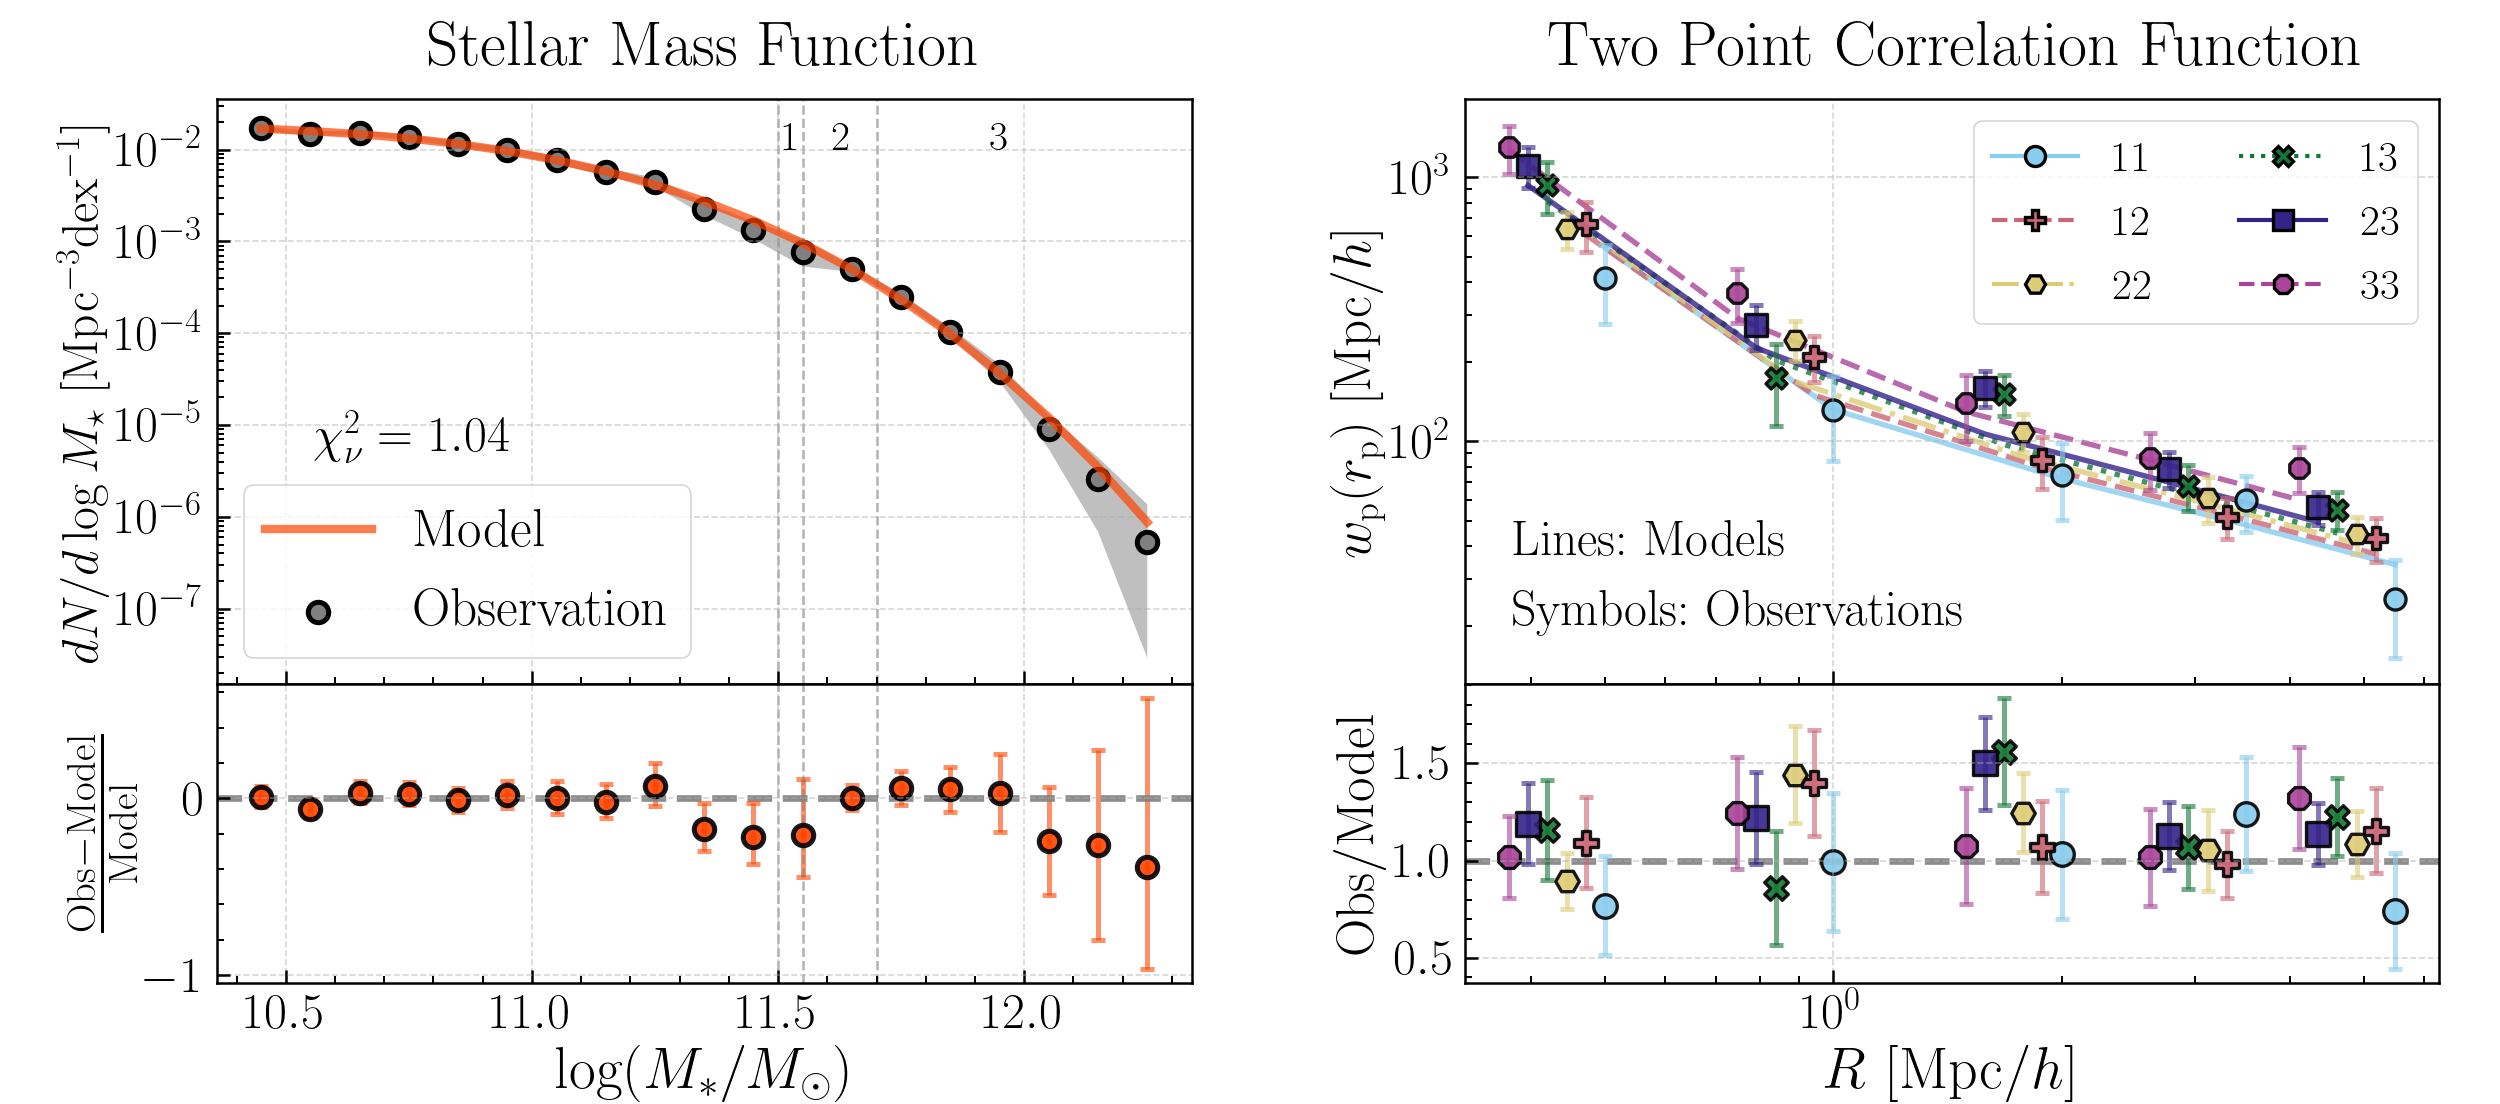
\includegraphics[width=0.8\textwidth]{figure/topn_fig_3}
  \caption{
      \textbf{Left} panels demonstrate how well the model (red line) can fit the observed SMF
      (grey symbols; shaded regions are uncertainties) that combines data from HSC at high-\mstar{}
      end and \texttt{PRIMUS} survey at low-\mstar{} end.
      The bottom sub-panel shows the relative residual of the best-fit SMF.
      The three vertical dashed-lines highlight the \mstar{} boundaries of the three \mstar{}-bins
      ([$11.50$, $11.55$, $11.70$]) used for measuring the two--point correlation functions of massive
      HSC galaxies.
      \textbf{Right} panels summarize the observed clustering of HSC massive galaxies (symbols)
      and their best-fit models (lines).
      [11, 22, 33] are the auto-correlation functions of the three \mstar{} bins, while
      [12, 13, 23] indicate the cross-correlation functions among the three bins.
      The bottom sub-panel shows the ratio between the observed and the model clustering signals.
    }
  \label{fig:best_mock}
\end{figure*}
%% ---------------------------------------------------------------------------------------------- %%

%% ---------------------------------------------------------------------------------------------- %%
%% HSC Model
%% ---------------------------------------------------------------------------------------------- %%
\section{Scaling relation model calibrated to match HSC observations}
    \label{app:hsc_model}

    In \S \ref{sec:estimate_scatter}, we describe the method to predict the stacked \dsigma{}
    profile of a sample of number density selected halos with certain \scatterMhaloObsSym{} value
    based on a $\log$-normal scaling relation with fixed slope ($\alpha=1$).
    This simple model helps us predict the \dsigma{} profiles for the four \topn{} bins
    as shown in Figure \ref{fig:mdpl2}.
    Meanwhile, to evaluate the impact of satellite galaxies on the \topn{} tests, we still need
    a mock catalog from simulation that can fit basic HSC observations of massive galaxies and
    have realistic satellite fraction at high-\mstar{} end.

    Taking advantage of the flexible modeling framework by (Bradshaw et. al. in prep.), we
    create such a mock catalog that can reproduce the SMF and clustering statistics of HSC massive
    galaxies.
    The model is a variant of the sub-halo abundance matching model (SHAM) presented in
    \citet{Lehmann2017} (also known as the ``$\alpha$ model'') that marginalizes over more than
    one halo properties to perform SHAM to.
    Instead of using the virial velocity ($v_{\rm vir}$) and maximum circular velocity ($v_{\rm Max}$),
    of halos as in \citet{Lehmann2017}, we decide to use the use a combination of \plan{XX} and
    \plan{XX; \mhalo{}?}.
    \song{Chris, please help fill the blank}
    We also use this model to constrain the SHMR and its scatter at high-\mhalo{} end.
    In particular, we model the SHMR using the functional form from \citet{Behroozi2013} but
    fixing the slope at low-\mhalo{} end ($\beta$).
    In total, the model has six free parameters:
    1. The $alpha$ parameter from \citet{Lehmann2017} model that determines the relative
       importance of halo properties;
    2. The four parameters that govern the mean SHMR at high-\mhalo{} end from \citet{Behroozi2013};
    3. And the scatter of \mstar{} at fixed \mhalo{}.

    As shown in Figure \ref{fig:best_mock}, the best-fit model can reproduce the observed
    mass function and clustering statistics of massive galaxies reasonably well.
    To ensure the model can fit the SMF beyond just the high-\mstar{} end, we adopt a ``hybrid''
    SMF: we use the complete sample of HSC massive galaxies at $0.2 < z < 0.5$ to cover the
    \logms{}$>11.5$ range, and use the \texttt{PRIMUS} $0.3 < z < 0.4$ SMF
    (\citealt{Moustakas2013}) for the $10.5 <$\logms{}$<11.5$ range.
    Both the HSC and the \texttt{PRIMUS} \mstar{} are from the \texttt{iSEDfit} code under very
    similar assumptions of stellar population properties.
    The \mstar{} of the HSC sample is based on our customized 1-D profile that capture the
    luminosity beyond 100 kpc, while the \texttt{PRIMUS} sample is based on small aperture
    photometry.
    Using the \texttt{PRIMUS} galaxies that also have the HSC 1-D \mstar{} measurements from
    \citet{Huang2018b}, we derive a simple constant offset term that help us ``stitch'' the two
    SMFs together.
    We note that this just ensures a smooth SMF for the fitting, and does not affect any results
    in this work.
    As for the clustering signals of HSC massive galaxies, we compute the auto- and
    cross-correlation signals after separating the sample into three \mstar{} bins: $11.50
    <$\logms{}$\leq 11.55$, $11.55 <$\logms{}$\leq 11.70$, and \logms{}$> 11.70$.
    The best-fit SHMR is broadly consistent with previous works including the scatter of
    \mstar{} value (\plan{$\sim 0.2$ dex}).
    More importantly, the satellite fraction at high-\mstar{} end is \plan{XX}, which is also
    similar to the results of previous works.
    We also verify that the satellite fraction value is robust to small changes in abundance
    matching methodology.

%% ---------------------------------------------------------------------------------------------- %%
%% Satellite v.s. Central
%% ---------------------------------------------------------------------------------------------- %%
\section{\dsigma{} profiles of centrals and satellites}
	\label{app:sat_cen}

    \todo{Placeholder}
    To calculate the LOS distance, we use the best available redshift and ignore its uncertainty.
    We have explored different choices of the cylinder size to make sure our result is robust.
    Furthermore, replacing \mmax{} with other larger aperture \mstar{} when identifying
    satellites does not change our result.
    
    \chris{We probably want a bit more of a why here -- impact is small, especially in high mass bins?}

%% ---------------------------------------------------------------------------------------------- %%
%% Figure: satellite v.s. central
%% ---------------------------------------------------------------------------------------------- %%
  \begin{figure}
      \centering
      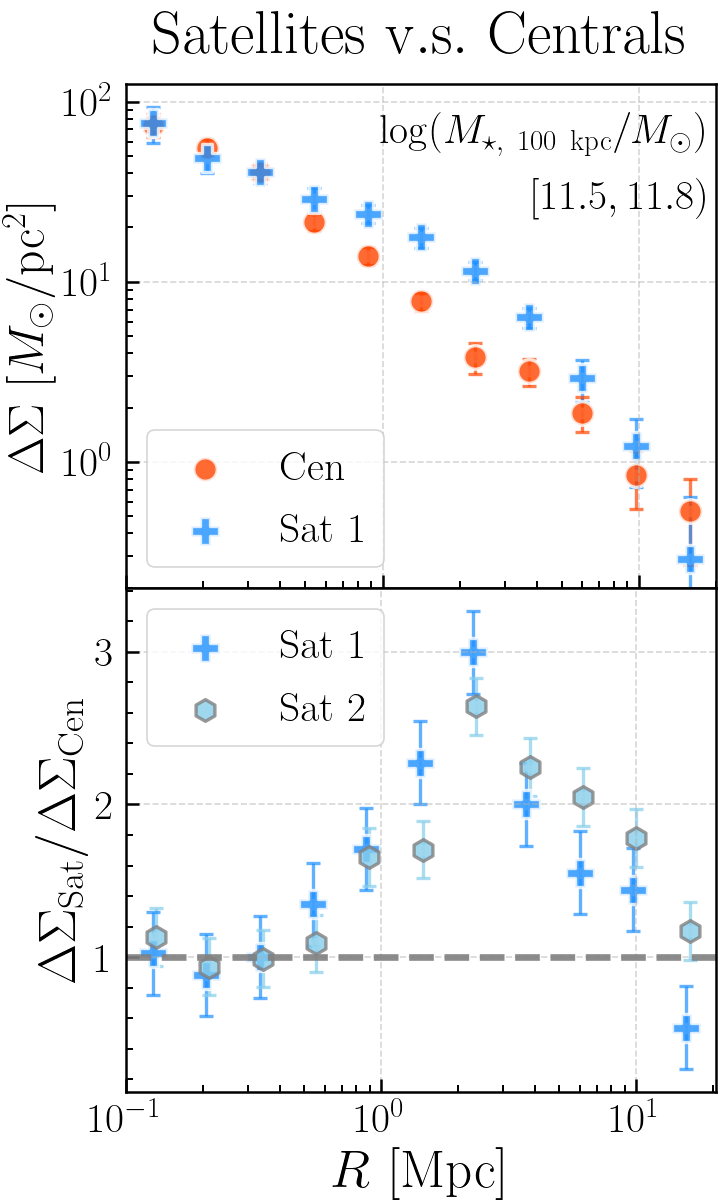
\includegraphics[width=0.47\textwidth]{figure/topn_fig_appendix_4}
      \caption{
          \todo{Placeholder}
          The relations between scatter of halo mass and the cumulative number density of each
          \topn{} bin for diffeent \mhalo{} proxies.
      }
      \label{fig:sat_cen}
  \end{figure}
%% ---------------------------------------------------------------------------------------------- %%

%% ---------------------------------------------------------------------------------------------- %%
%% Galaxy size as potential halo mass indicator
%% ---------------------------------------------------------------------------------------------- %%
\section{Galaxy size as \mvir{} indicator}
	\label{app:size}

    \todo{Placeholder}

%% ---------------------------------------------------------------------------------------------- %%
%% Figure: test other halo mass proxies.
%% ---------------------------------------------------------------------------------------------- %%
  \begin{figure*}
      \centering
      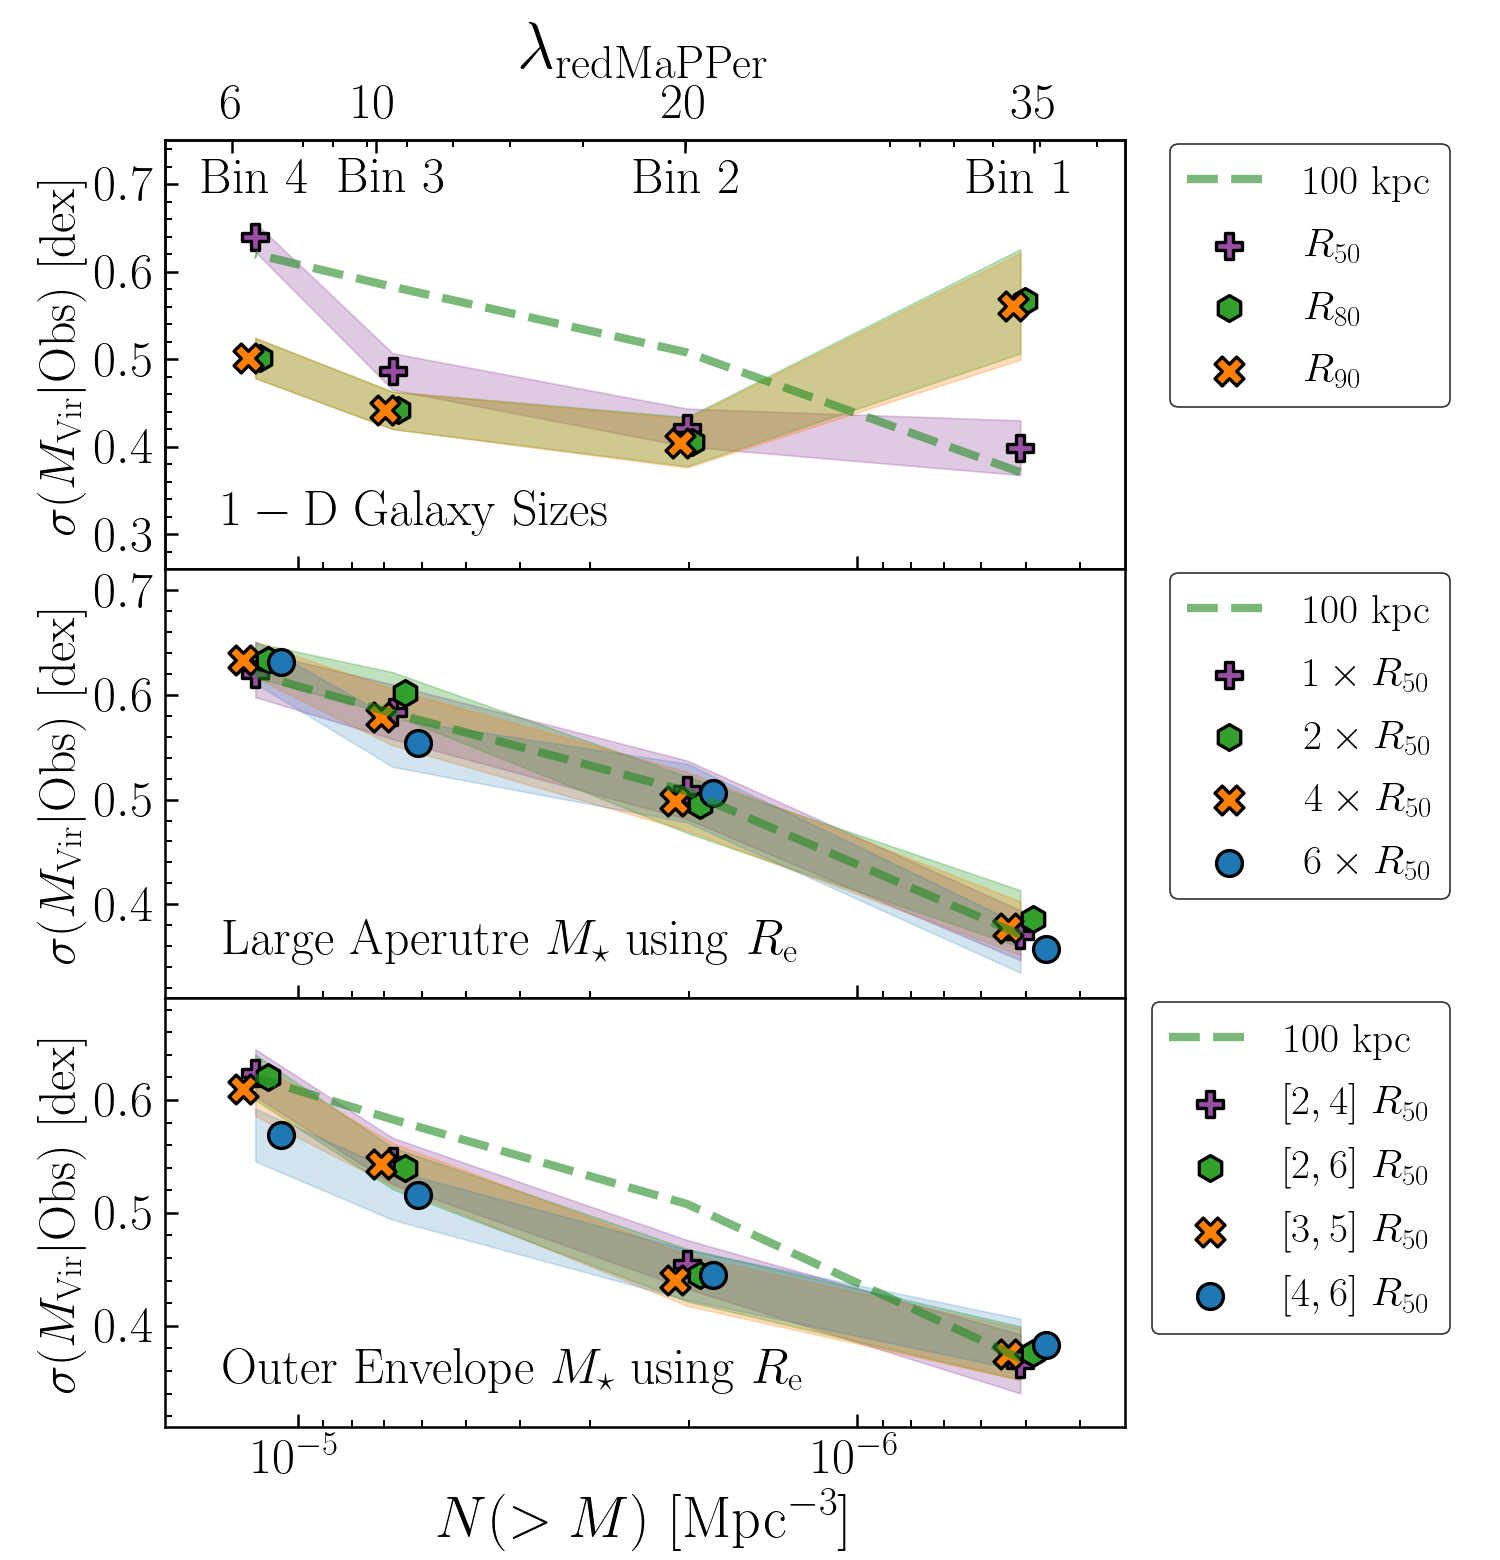
\includegraphics[width=13cm]{figure/topn_fig_appendix_2}
      \caption{
          The relations between scatter of halo mass and the cumulative number density of each
          \topn{} bin for different \mhalo{} proxies.
          The format is the same similar with Fig \ref{fig:scatter_trend}.
          \textbf{Top} panel shows the performance of different measurements of galaxy size as
          \mhalo{} proxies.
          We again use the trend of \maper{100} as the reference.
          \textbf{Middle} panel shows the trends for large aperture stellar masses defined by
          multiples of the half--light radius ($R_{50}$) instead of in physical kpc.
          \textbf{Bottom} panel is for the outer envelope \mstar{} defined by $R_{50}$.
      }
      \label{fig:scatter_trend_2}
  \end{figure*}
%% ---------------------------------------------------------------------------------------------- %%

%% ---------------------------------------------------------------------------------------------- %%
%% HSC v.s. SDSS redMaPPer
%% ---------------------------------------------------------------------------------------------- %%
\section{\topn{} results for SDSS \redm{} clusters}
	\label{app:sdss_redm}

    \todo{Placeholder}

%% ---------------------------------------------------------------------------------------------- %%
%% Figure: redMaPPer HSC v.s. SDSS
%% ---------------------------------------------------------------------------------------------- %%
  \begin{figure*}
      \centering
      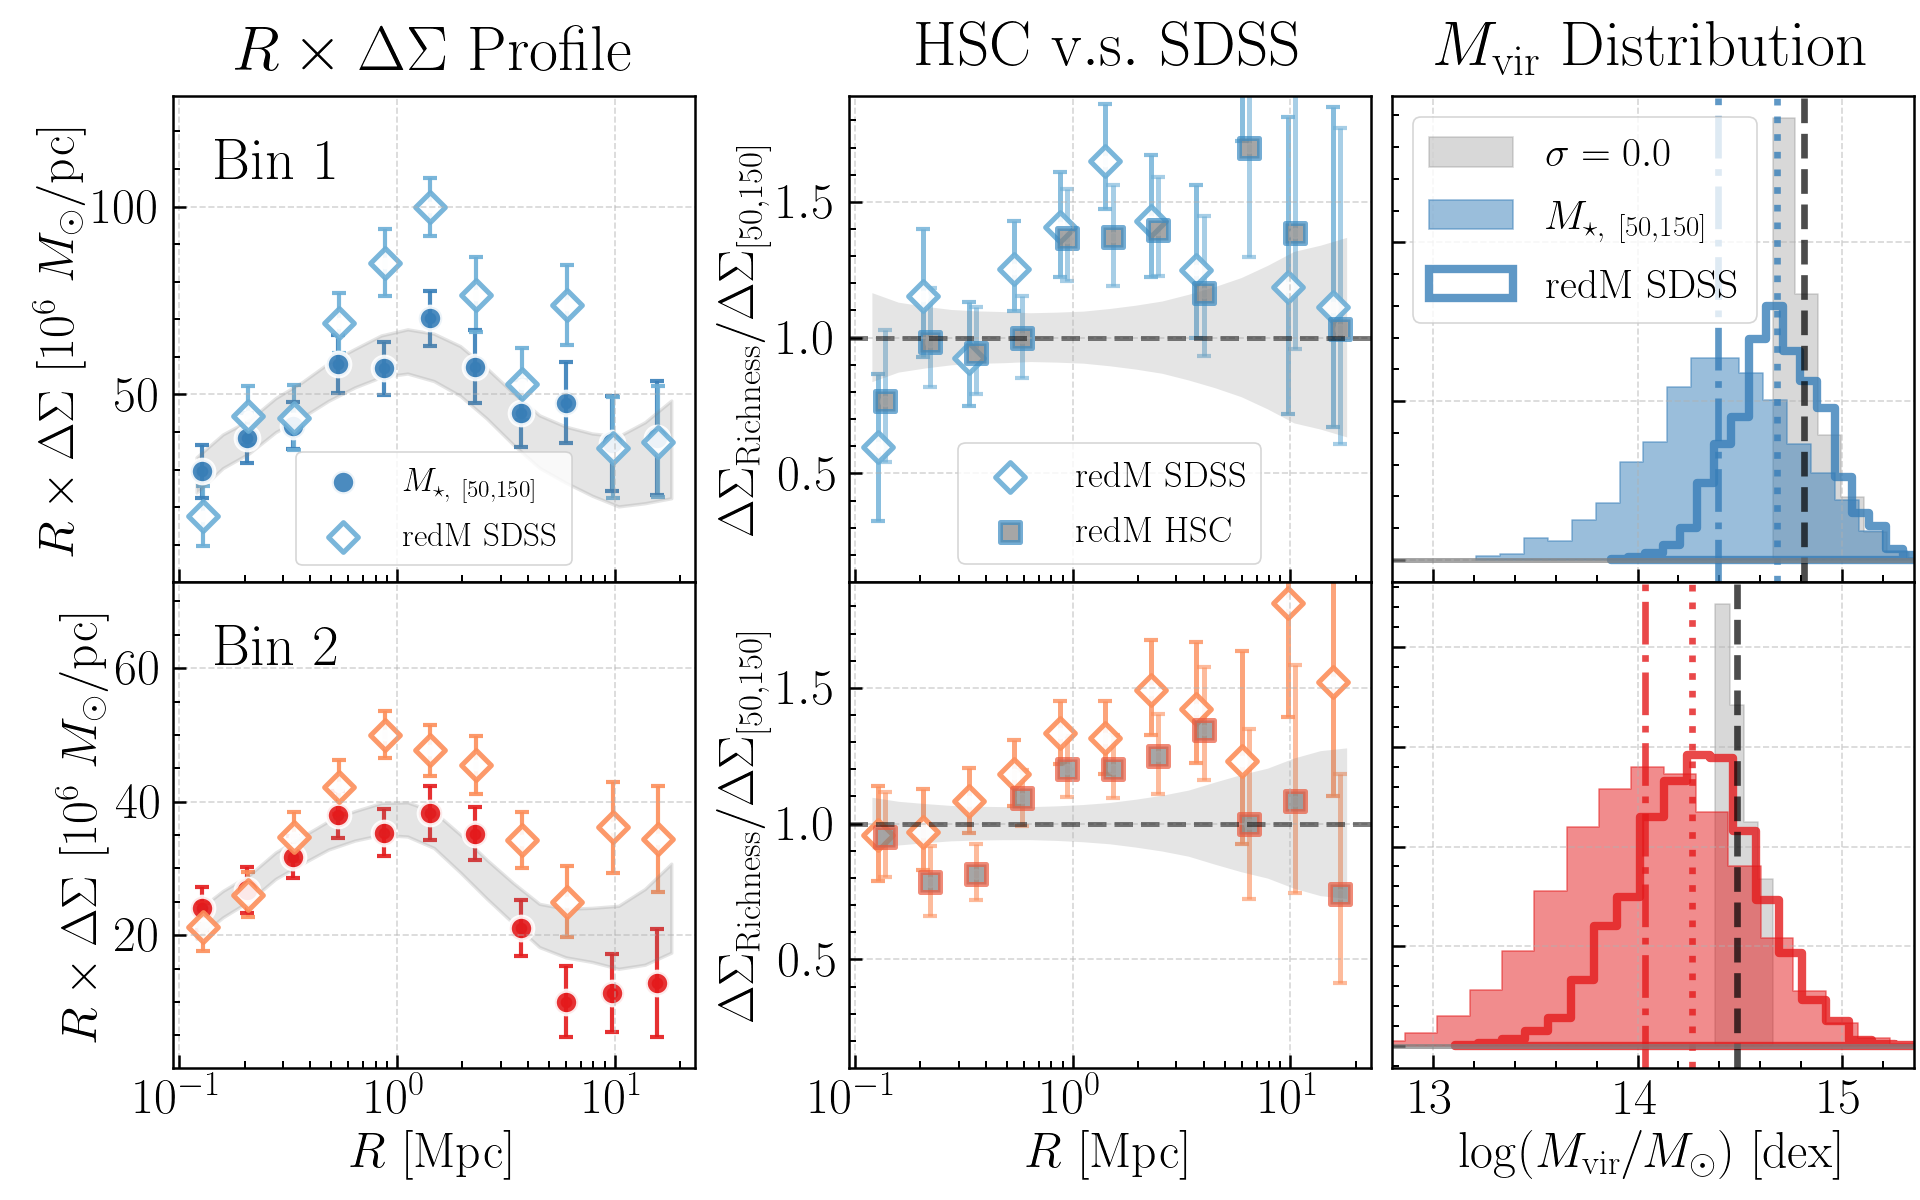
\includegraphics[width=\textwidth]{figure/topn_fig_appendix_3}
      \caption{
          Similar to Fig \ref{fig:mout_richness}, here we compare the lensing profiles of
          \redm{} clusters in the first two \topn{} bins using the SDSS \redm{} catalog.
          The layout of the figure is very similar to Fig \ref{fig:mout_richness}.
          \textbf{Left} panels compare the observed \rdsigma{} profiles of SDSS \redm{} clusters
          (open diamonds) and massive galaxies selected by \menve{50}{150} (solid circles).
          \textbf{Middle} panels show the ratio between the \dsigma{} profiles of the \redm{} clusters
          and the best-fit model profiles of the \menve{50}{150}-selected samples.
          We also compare the ratios using the SDSS \redm{} samples (open diamonds) to the
          HSC \texttt{S16A} \redm{} clusters (squares filled with grey color).
          In the same number density bin, the SDSS \redm{} sample shows higher overall lensing
          amplitudes and more prominent excess at $\sim 1$ Mpc than the HSC one.
          \textbf{Right} column compares the \mvir{} distributions predicted by \mdpl2{} simulation
          and also highlights the mean \mvir{} value in each bin.
      }
      \label{fig:sdss_redm}
  \end{figure*}
%% ---------------------------------------------------------------------------------------------- %%

%% ---------------------------------------------------------------------------------------------- %%
\bsp
\label{lastpage}
\end{document}

%% ---------------------------------------------------------------------------------------------- %%
%% ------ End of the File ------
%% ---------------------------------------------------------------------------------------------- %%
